\documentclass[a4paper,10pt,BCOR=15mm]{scrbook}
\usepackage[T1]{fontenc}
\usepackage[utf8]{inputenc}
\usepackage{epsfig}
\usepackage{amssymb,amsmath,amsthm,mathrsfs,mathtools,amscd}
\usepackage{natbib}
\usepackage{array}
\usepackage{lmodern}
\usepackage[all,cmtip]{xy}
\usepackage{graphicx}
\usepackage{float}
%\usepackage[left=4cm,right=3.5cm,top=3cm,bottom= 2.5cm]{geometry} 
\usepackage[bookmarks=true]{hyperref}


\DeclareMathOperator{\dive}{div}
\DeclareMathOperator{\grad}{grad}
\DeclareMathOperator{\spann}{span}
\DeclareMathOperator{\nulli}{null}
\DeclareMathOperator{\ind}{ind}
\DeclareMathOperator{\rank}{rank}
\DeclareMathOperator{\const}{const}

\providecommand{\abs}[1]{\lvert#1\rvert}
\providecommand{\norm}[1]{\lVert#1 \rVert}
\providecommand{\dupa}[2]{\langle #1,#2 \rangle}
\providecommand{\inva}[1]{\text{d} #1}
\providecommand{\andi}[0]{\quad \text{and} \quad}
\providecommand{\esssup}{\mathop{\mathrm{ess\,sup}}\displaylimits}


%opening
\title{Distributed Control of Semidiscretized Oseen Equations}
\author{Jan Heiland}

\begin{document}

\newtheorem{thm}{Theorem}[chapter]
\newtheorem{cor}[thm]{Corollary}
\newtheorem{lem}[thm]{Lemma}

\theoremstyle{plain}
\newtheorem{lema}[thm]{Lemma}


\theoremstyle{remark}
\newtheorem{exa}[thm]{Example}

\theoremstyle{remark}
\newtheorem{rem}[thm]{Remark}

\theoremstyle{definition}
\newtheorem{defin}[thm]{Definition}

\theoremstyle{plain}
\newtheorem{prob}[thm]{Problem}

\theoremstyle{plain}
\newtheorem{prop}[thm]{Proposition}

\floatstyle{ruled}
\newfloat{algorithm}{htbp}{loa}[chapter]
\floatname{algorithm}{Algorithm}


\bibliographystyle{plain}
\numberwithin{equation}{chapter}


 \begin{titlepage} 
\vspace*{7cm} 
 \begin{center} 
  \large 
 Diploma Thesis\\  
\vspace{1cm} 
\Huge 
Distributed Control of Semidiscretized Oseen Equations\\ 
 \vspace{2cm} 
  \large 

 Jan Heiland <heiland@math.tu-berlin.de>\\ 
March 16th, 2009\\

\vspace{1cm}

 \normalsize 
 \vfill 
Overseen by
Prof. Dr. Volker Mehrmann \\
and Priv.-Doz. Dr. Etienne Emmrich\\
\vspace{0.3cm}
Chair for Numerical Analysis\\
\vspace{1cm}
Faculty for Mathematics \\
TU Berlin
 \end{center} 
\end{titlepage}

%opening
%\chapter*{}
%\thispagestyle{empty}
%\vspace{10cm}
%Die selbstst\"andige und eigenh\"andige Ausf\"uhrung versichert an Eides statt


%\vspace{1cm}
%Berlin, den

%\quad
%\newpage
%\thispagestyle{empty}


%\setcounter{page}{2}

\newpage 
\thispagestyle{empty}
\quad 


\chapter*{Verteilte Kontrolle von ortsdiskretisierten Oseen Gleichungen}


Diese Diplomarbeit behandelt ein Verfahren zur mathematischen Modellierung von Strömungsbeeinflussung. 

In vielen Anwendungsbereichen, wie z.B. in der Aerodynamik von Fahrzeugen, ist aktive Str\"omungsbeeinflussung oder -kontrolle von Bedeutung. Aktuelle Forschungen liefern gute Ergebnisse, vgl. [71], diese aber vor allem in praktischen oder numerischen Experimenten. Im Allgemeinen sind die Untersuchungen und Experimente sehr komplex und aufw\"andig, was nicht zuletzt an der sehr rechenintensiven Modellierung von Str\"omungen liegt.

Ein wesentlicher Beitrag der Mathematik zur Behandlung von Str\"omungsbeeinflussung liegt in der Entwicklung und Analyse von Methoden zur Modellreduktion (MOR). Ein \"Uberblick zu (MOR) Ans\"atzen findet man z.B. in [3]. 

Ein allgemeines Modell zur Str\"omungskontrolle besteht zun\"achst aus einem Modell f\"ur die betrachtete Str\"omung. In den meisten F\"allen wird daf\"ur die Navier-Stokes Gleichung zur Beschreibung des Geschwindigkeits- und des Druckfeldes eines inkompressiblen Fluids in einer gegeben Umgebung und einem festen Zeitabschnitt verwendet, vgl. [49]. Zur Modellierung der beeinflussenden Gr\"oßen wird das Modell um einen Term zur Beschreibung der verteilten Kontrolle $u$ aus einem Inputraum $\mathcal U$ erweitert. Verteilte Kontrolle bedeutet hierbei, dass die Kontrollfunktion als stetig im Raum verteilt definiert ist, was insbesondere die Betrachtung von punktweiser und Kontrolle \"uber den Rand ausschließt.

Das Systemverhalten wird \"uber den Output $y \in \mathcal Y$ verfolgt, der mittels eines Operators aus dem Druck- und Geschwindigkeitsfeld erzeugt wird. Abbildung (Figure) 1.1 zeigt ein zweidimensionales Beispiel. 

Die hier vorgeschlagene Reduktion des allgemeinen Modells, basiert auf den Untersuchungen von Schmidt [92] und verwendet die Oseen-Linearisierung der Navier-Stokes Gleichungen zur Str\"omungsmodellierung und endlichdimensionale Kontroll- und Beobachtungsr\"aume $\mathcal U$ und $\mathcal Y$. In Kombination wird so die Verwendung einer endlichdimensionalen linearen \textit{i/o map}, welche die Kontrolle direkt auf den Output abbildet, erm\"oglicht. Dieser Ansatz ist motiviert durch zwei Beobachtungen. Einerseits geschieht aktive Strömungskontrolle oft lokal im Ort und in der Zeit, weshalb der Linearisierungsfehler klein gehalten werden kann. Zweitens haben komplexe Systeme oft ein relativ einfaches Input/Output Verhalten, das auch mit endlich dimensionalen Ein- und Ausgaben gut angen\"ahert werden kann.

Das übergeordnete Ziel ist es, eine kompakte mathematische Formulierung zu entwickeln, die eine effiziente Realisierung in numerischen Simulationen von Strömungsbeeinflussung ermöglicht. Dazu werden in jedem Kapitel dieser Diplomarbeit beide Grundkonzepte, d.h. die lineare Oseen Gleichung und die diskrete Kontrolle dergleichen mittels einer \textit{i/o map} untersucht.

Zunächst werden in Kapitel \textbf{2 Zugrundeliegende Gleichungen und Kon- zepte} die beitragenden Gleichungen und der mathematische Rahmen zur Behandlung derselbigen vorgestellt. Als Basis für die Modellierung der Strömung werden verschiedene Typen von Oseen Gleichungen und deren schwache Formulierung, zusammen mit Aussagen zur Existenz und Eindeutigkeit von verallgemeinerten Lösungen, angegeben. Desweiteren werden die grundlegenden Ideen und Formeln zur mathematischen Formulierung von Strömungsbeeinflussung angesprochen und die notwendigen Konzepte zur Formulierung und Behandlung von diskreten \textit{i/o maps} bereitgestellt.

Kapitel \textbf{3 Kontrolle der ortsdiskretisierten Oseen Gleichungen mittels \textit{i/o maps}} bringt beide Konzepte in einer expliziten Formel zusammen. Dazu werden zunächst die Oseen Gleichungen im Ort diskretisiert und als ein System von differentiell algebraischen Gleichungen interpretiert. Damit kann eine explizite Formel für die Lösung der semidiskretisierten Oseen Gleichung angegeben werden, die durch einen zusätzlichen Term zu einer Lösungsformel des kontrollierten Systems erweitert wird. Eine weitere Umformulierung ergibt dann eine explizite Darstellung für die\textit{ i/o map}. Formuliert man diese Abbildung für diskrete Räume, kann eine Matrixdarstellung hergeleitet werden.

Kapitel \textbf{4 Fehleranalyse der Oseen \textit{i/o map}} enthält Abschätzungen für den Fehler, der durch die Verwendung der endlichdimensionalen Darstellung der \textit{i/o map} verursacht wird. Außerdem werden die weiteren Fehlerquellen, die Ortsdiskretisierung und die numerische Integration der kontrollierten Oseen Gleichungen angesprochen.

Kapitel \textbf{5 Numerische Behandlung der Zustandsgleichungen} befasst sich mit der Umsetzung des mathematischen Modells auf dem Computer. Zur Realisierung der Ortsdiskretisierung wird für ein 2D Modellproblem die $Q_1P_0$ methode, eine finite Elemente Methode, welche die Geschwindigkeit stückweise bilinear und den Druck stückweise konstant annähert, vorgestellt. Im zweiten Teil wird eine Adaption des \textit{Projection2} Algorithmus für die $Q_1P_0$ diskretisierte Oseen Gleichung angegeben. 

Kapitel \textbf{6 Numerische Tests} enthält die Implementierung und Ergebnisse von im Rahmen der Arbeit untersuchten Testproblemen. Dafür wurde die Kontrolle einer 2D Strömung in einer Kavität mittels der Oseen Gleichung modelliert. Insbesondere wurde eine konkrete \textit{i/o map} für mittels Wavelets diskretisierte In- und Outputräume berechnet und dazu verwendet, ein vorgege- benes Ströumgsbild mit Hilfe von Kontrolle zu erreichen.

Das abschließende Kapitel beinhaltet zusammenfassende Bemerkungen und einen Ausblick auf sich anschließende Untersuchungen. 


%\begin{abstract}
%The main goal of the diploma thesis is to capture the input/output (i/o) behaviour of a physical system governed by the linear Oseen equations in a closed mathematical formulation to enable an effective application of distributed control. A practical approach is to discretize the spaces of the input and output functions, to obtain an approximating matrix representation of the i/o operator. Considering the semidiscretized Oseen equation as a linear differential algebraic equation (DAE) with constant coefficients, one has an explicit solution formula. If applied to a system with a control term, it can function as the base for a closed-form i/o map. This approach admits a wide range of spatial discretization methods, a special focus lies on mixed $Q_1P_0$ finite elements. The investigation is accompanied and backed by numerical tests. 
%\end{abstract}


\tableofcontents

\chapter{ Introduction}
\section{Motivation}
When in the 1950s the first signs of the progress that computers were about to bring to applied mathematics appeared, Jonathan von Neumann predicted: ``The computer will enable us to divide the atmosphere at any moment into stable regions and unstable regions. Stable regions we can predict. Unstable regions we can control.'', as cited by \cite[p. 219]{dyso}. At least with the estimation that this is only a matter of a decade von Neumann was wrong. Up to now the research concerned with the control of flows, ranging from large scale problems as e.g. the control of the weather to macro scale applications as the active flow control by means of piezoelectrical devices, see e.g. \cite{piezo}, is of high relevance, with great potential for real life application, as e.g. for aeronautics, see \cite{gadel,gunzo}.

Recent developments come up with good results for real life applications, see e.g. \cite{king}, in particular for experimental or numerical investigations. The mathematical analytical treatment of problems referring to flow control is still at an early stage. This may be due to the fact, that as stated e.g. in \cite{bewley} the mathematical analysis of flow control unites essential and non-trivial parts of the complex fields fluid-dynamics, Navier-Stokes mathematics, control theory, numerical analysis and optimization.

In view of flow control many mathematical research directions are trying to close the gap in practical relevance between best practice heuristic methods and a purely mathematical approach, with e.g. guaranteed robustness and convergence rates. Basically, these are connected to the mathematical modeling of the control-systems, the analysis of system-theoretic properties as well as the development of performant methods for the practical realization, as e.g. linear algebra tools, goal oriented discretizations, problem specific codes and model reduction.

This work aims at the distributed control of a physical system governed by the Navier-Stokes equations for variable time $t\in[0,T]$, as illustrated schematically in Figure \ref{inoupic}. The physical system is perturbed by an input $u$ belonging to an input space $\mathcal U$. The effect of this manipulation is observed via sensors measuring physical quantities and thus generating the output $y\in \mathcal Y$ of the system for the given control.

\begin{figure}[htbp]
\begin{center}
 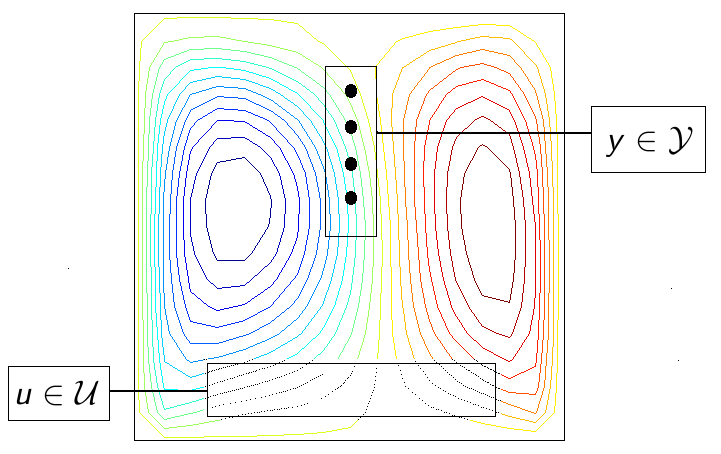
\includegraphics[width=9cm]{system.png}
 \caption{Schematic illustration of a 2D flow system perturbed by an input $u$ and observed via sensors extracting the output $y$ from the actual state }
 \label{inoupic}
\end{center}
\end{figure}

 Distributed means that the considered control $u(t)$ applied to the system is distributed in space, i.e. $u(t) = u(t;\sigma)$ with a space variable $\sigma$ varying smoothly distributed in a subdomain of the considered flow domain. This excludes the application to control acting pointwise or at the boundary. 

On the way to enable an effective control or optimization of the system, i.e. finding means or models for a mathematically understood and numerically affordable method to perturb a flow so that a certain state of the flow is achieved, basically two concepts are put together. First the nonlinear semidiscretized Navier-Stokes equations are linearized, giving the Oseen approximation of the considered flow equations. The use of the Oseen equations means a modification of the considered state system. Then the model of the control design is reduced by discretizing the admitted inputs and the outputs. Both, the linear state space system and the discrete input and output spaces enable the use of a discrete linear input/output (i/o) operator, mapping the input $u$ directly onto the system output $y$.

This joint approach is motivated by the observation, that control often acts locally in time, and therefore a linearization promises still a good approximation. Secondly, the matrix representation of a discrete linear i/o map enables an effective control of the system. 

The practical relevance, which is actually the control of the Navier-Stokes system, may be maintained by coupling the control of the Oseen to the control of the Navier-Stokes equations via an iteration as illustrated in Figure \ref{optscheme}. Thus, it can be ensured that the Oseen approximation is sufficiently close to the Navier-Stokes equations system for the actual state.

\begin{figure}[htbp]
\begin{equation*}
\boxed{
 \xymatrix{
u  \ar[rr] & &*+=[F-,]\txt{~NSEs~ }\ar[dd] \ar[r] &C^Tv_n \stackrel{!}{=}y^* \ar[ddl]|-{\text{~~~~Linearization about $v_n$}}  \\  & & & \\
 & \bar u_n^k \ar[r] &*+=[F-,]\txt{~Oseen~ } \ar[r] &C^T\bar v_n^k \stackrel{!}{=}\bar y^* \ar[ld] \\
\bar u_{n}^* \ar[uuu]|- {~~n \leftarrow n+1} & &\framebox{Control} \ar [ll] \ar[lu]|- {k \leftarrow k+1 }  &
}
}
\end{equation*}
\caption{Scheme for optimal control of the Navier-Stokes equations via an iterative coupling to the Oseen linearization. First for a control $u_n$ the state $v_n$ of the system, governed by the Navier-Stokes equations, is computed. If the output $C^Tv_n$ does not match the target output $y^*$, the Oseen linearization about $v_n$ of the Navier-Stokes equations is used to compute the approximated optimal control $\bar u_{n}^*$ of the Oseen system with respect to the adapted target state $\bar y^*$. This is done in an inner iteration over $k$. Then $\bar u_{n}^*$ serves as the basis for an improved $u_n$ in the next step of the outer iteration over $n$.}
\label{optscheme}
\end{figure}

This work, dealing with distributed control of the semidiscretized Oseen equations, contributes to the presented work flow in Figure \ref{optscheme} in view of finding the optimal control $\bar u_{n}^*$ for the Oseen approximation. 

\section{Overview of the Topic}
The basis of the investigation is a mathematical model of the flow control design. In general a partial differential equation (Navier-Stokes, Oseen or Stokes) model of the physical flow system is taken and extended by model parameters representing actuators and sensors, as described e.g. in the monographs \cite{bens1,bens2}. The validity of the model may be sensitive with respect to the model parameters. Considering for example a control design on the basis of the incompressible Navier-Stokes equations, a perturbation in the continuity equation may necessitate a change to a model which is capable to describe the behaviour of compressible fluids, c.f. \cite{feirei}.

To model the distributed control where the model parameters are distributed in space the right-hand side in the momentum equation is adjusted, as used e.g. in \cite{betezi,dehi,guhosv,guma,hesosu,hinz}. The actuation of the flow via the boundary, i.e. via the boundary conditions in the partial differential equation model, is beyond the scope of distributed control. This issue is addressed e.g. in \cite{guma2,hiku,hosv}.

In the present case the considered model bases on the unsteady Oseen equations. The partial differential equations are transformed into a differential algebraic equation system by means of a semidiscretization eliminating the dependency on the space variables. A general discussion on flow equations as a differential algebraic equation systems is given in the works by Weickert \cite{weic,weic2}. 

For the obtained linear differential algebraic equation system with constant coefficients an explicit solution formula is derived using the general theory for differential algebraic equations provided e.g. in \cite{mehr} and the specific results for flow-connected differential algebraic equations given in \cite{emme}.

The explicit solution formula for the Oseen system, adapted to the control design, functions as an explicit input/output map.

The existence of an explicit formula for the input/output behaviour simplifies the control design model. In most cases, however, a \textit{model order reduction} is necessary for a practical realization. An overview of the wide range of \textit{model order reduction} theory and techniques is presented e.g. \cite{antou,bemeso}. 

In this thesis an order reduction for the input/output map is carried out by discretizing the input and output spaces, so that a finite dimensional representation of the input/output map can be computed. This approach was introduced by Schmidt \cite{schm} in a semigroup context. The related concept of balanced truncation for the spatially discretized linear Stokes and Oseen approximations are studied in \cite{hesosu,stykel}.

The finite dimensional input/output map enables an effective realization of optimal control for the Oseen equations. As motivated above, the Oseen approximation will be used in an iteration aiming at the optimal control of the Navier-Stokes equations. The publications \cite{betezi,dehi,gunzo,guhosv,guma,guma2,hesosu,hiku,hinz,hosv} represent a small selection of contributions on the optimal control of Navier-Stokes equations. 
Results regarding the optimal control of the steady-state Oseen equations are presented e.g. by Po{\v s}ta and Roub{\'\i}{\v c}ek \cite{poro}. The unsteady case is studied e.g. by Bewley et. al. \cite{betezi}. The control of the Stokes equations with respect to the control of the Navier-Stokes equations is e.g. studied in \cite{constonse}.

Finally the numerical realization of a control design often requires additional efforts, since many commercial and academic simulation codes are designed for static simulations without an interface to a control unit. Environments for the simulation of control problems are provided e.g. by \textsc{Matlab} and \textsc{Scilab} \cite{scilab,matconbo}. Further approaches and tools, coupling control and flow simulations, are presented in \cite[Ch. 5]{schm} and \cite{slawig}.

\section{Chapter Outline}

The two basic issues treated in every chapter of this work are the modeling of the flow problem by spatial discretization and the control thereof. The overall goal is to bring both together in a condensed mathematical formulation that is suitable for application.

Thereto, chapter \textbf{2 Basic Equations and Concepts} starts the thesis with an explanation of the models and concepts used and with providing the mathematical framework for their analysis. Regarding the model the Oseen equations are derived from the Navier-Stokes equations (NSEs) and formulated in a weak context. Also, results regarding existence and uniqueness of solutions are stated. Secondly the essential ideas and mathematical formulation in regard to the control of flows are presented. Thirdly, the mathematical theory and realization of discrete input/output maps (i/o maps) is introduced.

Chapter \textbf{3 Control of Spatial Discretized Oseen via I/O Mapping} is the core of the thesis, since it connects the spatially discretized flow equations with the input and output functions in one explicit formula. This requires the formulation of the spatial discretization of the Oseen equations, followed by the formulation as a differential algebraic equation (DAE) system, for which an explicit solution formula is established. The application to distributed control is realized by extending the formula to the controlled system. On the basis of the explicit formula an explicit representation of an linear i/o map for the Oseen system is derived.

Approximating the i/o map by a finite dimensional matrix representation may reduce the computational load within an optimization. The consistency error of this model order reduction method is estimated in chapter \textbf{4 Error Analysis of the Oseen I/O Map}. Besides the signal approximation error also the error due to the spatial discretization of the Oseen equations and the time integration error are briefly addressed.

The chapter \textbf{5 Numerical Treatment of the State Equations} addresses the discretization schemes used within this investigation to solve the Oseen equations numerically. Regarding the spatial discretization the $Q_1P_0$ finite element is discussed, along with the necessary pressure stabilization. The second part provides an application of the \textit{Projection2} algorithm presented in \cite{grea} to the $Q_1P_0$ discretized Oseen equations.

Chapter 6 \textbf{Numerical Tests} contains the setup and the results for the numerical investigation of the above concepts on the basis of a model of a 2D driven cavity flow. 

The last chapter completes this work with summarizing conclusions and remarks and with an outlook on future tasks connected to the topic of this thesis.

\chapter{Basic Equations and Concepts}
\section{Incompressible Flow State Equations}
Let $\Omega$ denote a Lipschitz domain in $\mathbb R ^ n$, $n=2,3$ and let $\partial \Omega$ denote its boundary. For an exemplary illustration the dimensionless Navier-Stokes equations on a time interval $(0,T]$, represented by the momentum equation
\begin{subequations}\label{nsee}
\begin{align}
 v_t +(v \cdot \nabla) v+\nabla p - \frac{1}{Re} \triangle v  &=  f \quad \mbox{in } \Omega \times (0,T] 
\intertext{the divergence free constraint}
\nabla \cdot v &= 0 \quad \mbox{in } \Omega \times (0,T] 
\end{align}
\end{subequations}
together with completing initial and homogeneous Dirichlet boundary conditions 
\begin{equation*}
 v \vert _ {\partial \Omega} = 0 \quad \andi{} v \vert _{t=0} = v_0
\end{equation*}
is considered. The above equations describe the motion of an incompressible Newtonian fluid with constant density by the states of the velocity $v$ and the dynamic pressure $p$, representing the physical pressure divided by the density. The right hand side $f$ describes the field of the external forces, the \textit{Reynolds number} $Re = V_\infty L / \nu$ contains the specific flow characteristics, i.e. the length scale $L$, a characteristic velocity $V_\infty$ of the flow and the dynamic viscosity $\nu$ of the medium. 

The dimensionless formulation of the NSEs is obtained by scaling the physical quantities describing time, location, velocity and pressure in the flow modeling equations by characteristic values. For a detailed derivation and discussion of the physical and the dimensionless NSEs the reader is referred to standard works on fluid dynamics, as e.g. \cite{lalifl,loj}.

\subsection{Spaces, Norms and Forms}

In view of the finite element discretization approximation of the flow equations discussed in the later sections and applied in the numerical experiments, this chapter briefly introduces the framework for a weak formulation of the NSEs and its linear approximations. More detailed expositions are provided e.g. in \cite{gira2,gunz,sohr,tema}.

Let $L^2(\Omega)$ denote the space of functions that are square integrable over $\Omega$ and equipped with the inner product and norm
\begin{equation*}
 (p,q) = \int _ \Omega pq \text{ d} x \quad \text{and} \quad \norm{q}_0 = (q,q) ^ {1/2}
\end{equation*}
respectively. With regard to the pressure, which is determined by \eqref{nsee} only up to an arbitrary additive constant, the constrained space
\begin{equation*}
 L_0^2(\Omega) = \left \{ q \in L^2(\Omega) : \int_\Omega q \inva{x} = 0 \right \}
\end{equation*}
is introduced. Denoting by $\partial ^ \alpha q$ the weak derivative of $q$ with respect to the multiindex $\alpha$, for any non-negative integer $m$ one can define the Sobolev space
\begin{equation*}
 H^{m}(\Omega) = \left \{ q \in L^2(\Omega) : \partial ^ \alpha q \in L^2(\Omega), \forall \abs{\alpha} \leq m \right \}  
\end{equation*}
On this class of Sobolev spaces an inner product and the associated norm
\begin{equation*}
 ((p,q))_m = \sum _ {\abs{\alpha} \leq m } (\partial ^ \alpha p, \partial ^ \alpha q)  \andi{} \norm{q}_m = ((q,q))_m ^ {1/2}
\end{equation*}
respectively, and a semi-norm
\begin{equation*}
 \abs{q}_m =\bigl ( \sum _ {\abs{\alpha} = m } (\partial ^ \alpha p, \partial ^ \alpha q)  \bigr ) ^ {1/2}
\end{equation*}
can be defined. One has $L^2(\Omega) = H^0(\Omega)$ and $H^1(\Omega)$ is the space of all square integrable functions over $\Omega$ with all its weak derivatives of first order in $L^2(\Omega)$.  Together with its subspace 
\begin{equation*}
 H^1_0(\Omega) = \left \{ q \in H^1(\Omega) : q =0 \text{ on } \partial \Omega \right \}  
\end{equation*}
$H_0^1(\Omega)$ is of particular interest with respect to the NSEs with homogeneous Dirichlet boundary conditions. The condition $q = 0$ on $\partial \Omega$ is short written for $q\vert _{\partial \Omega} = 0$ in $L^2(\partial \Omega)$, i.e. $q$ equals zero everywhere on the boundary of $\Omega$ except on a set of $\partial \Omega$ measure zero. 

The dual space of $H_0^1(\Omega)$, denoted by $H^{-1}(\Omega)$, contains the bounded linear functionals on $H_0^1(\Omega)$. A norm for $H^{-1}(\Omega)$ is given by
\begin{equation*}
 \norm{f}_{-1} = \sup _ {0 \neq q \in H_0 ^1(\Omega) }\frac{\dupa{f}{q} }{\abs{q}_1}
\end{equation*}
with $\dupa{f}{q}$ denoting $f(q)$. The use of $\abs{\cdot}_1$ is valid, c.f.\eqref{pfi}.

For vector valued functions of dimension $d$ the respective spaces and its elements are denoted by bold letters and defined as follows:
\begin{subequations}
\begin{align*}
 \mathbf L^2 (\Omega):= [L^2(\Omega)]^d =  \{ \mathbf v: v_i \in L^2(\Omega), i = 1, \dotsc , d \} \\
\intertext{as well as}
 \mathbf H ^1 _0 (\Omega):= [H_0^1(\Omega)]^d  \andi{}  \mathbf H^{-1} (\Omega):= [H^{-1}(\Omega)]^d 
\end{align*}
\end{subequations}


The respective inner products and norms are defined analogously to the example
\begin{equation*}
((\mathbf v, \mathbf w ))_1 = \sum _{i=1} ^ d ((v_i, w_i ))_1 \andi{} \norm{\mathbf v}_1 = \biggl [ \sum _{i=1} ^ d \norm{v_i} _ 1 ^2 \biggr ] ^{1/2}
\end{equation*}
To express the inner product of $\mathbf L ^2$ functions the scalar vector product is used
\begin{equation*}
(\mathbf v, \mathbf w ) = \int _\Omega \mathbf v \cdot \mathbf w \inva{x}
\end{equation*}

In $\mathbf H_0^1(\Omega)$ for a constant $C_{PF}$ depending on $\Omega$ the \textit{Poincare-Friedrichs inequality} 
\begin{equation}\label{pfi}
 \norm{\mathbf v}_1 \leq C_{PF} \abs{\mathbf v}_1, \quad \mathbf v \in \mathbf H_0^1(\Omega)
\end{equation}
holds, c.f. \cite[p. 59]{zeid}, implying that the semi-norm $\abs{\cdot}_1$ is equivalent to the norm $\norm{\cdot}_1$ and can be used instead. 

Now the following bilinear forms 
\begin{subequations}
\begin{align*}
 a(\mathbf v, \mathbf w)&= \frac{1}{Re}  \int _\Omega \grad \mathbf v : \grad \mathbf w \inva{x} \quad \text{for }  \mathbf v, \mathbf w \in \mathbf H^1 (\Omega)\\
  b(\mathbf v, q) &=  \int _\Omega q \dive \mathbf v \inva{x} \quad \text{for }  \mathbf v \in \mathbf H^1 (\Omega) \andi{} q \in L^2(\Omega)\\
\intertext{and the trilinear form}
c(\mathbf u,\mathbf v, \mathbf w) &= \int _\Omega \mathbf u \cdot \grad \mathbf v \cdot \mathbf w \inva{x} \quad \text{for } \mathbf u, \mathbf v, \mathbf w \in \mathbf H^1 (\Omega)
\end{align*}
\end{subequations}
can be defined using the notations $(\grad \mathbf v)_{ij} = \partial v_j / \partial x_i$ and
\begin{align*}
\grad \mathbf v:\grad \mathbf w &= \sum_{i,j=1} ^d \frac{\partial v_i}{\partial x_j} \frac{ \partial w_i }{ \partial x_j} \\
\mathbf u \cdot \grad \mathbf v \cdot \mathbf w &= \sum_{i,j=1} ^d u_j \frac{ \partial v_i }{ \partial x_j}w_i
\end{align*}

Related to functions belonging to $\mathbf H_0^1(\Omega)$ and $L_0^2(\Omega)$ the forms $a,b$ and $c$ have the following properties. Given $\mathbf u,\mathbf v \in \mathbf H_0 ^1 (\Omega)$ one has 
\begin{equation*}
 a(\mathbf u,\mathbf v) = \frac{1}{Re}(\mathbf u,\mathbf v)_1 \andi a(\mathbf v,\mathbf v) = \frac{1}{Re}\abs{\mathbf v}^2_1
\end{equation*}
and thus, using the \textit{Cauchy-Schwartz inequality} and recalling that $\abs{\cdot}_1$ is a norm on $\mathbf H_0^1(\Omega)$, one obtains boundedness and $\mathbf H_0^1(\Omega)$-coercivity of $a$, i.e.
\begin{equation}\label{coea}
 a(\mathbf u,\mathbf v) \leq \frac{1}{Re}\abs{\mathbf u}_1 \abs{\mathbf v}_1 \andi a(\mathbf v,\mathbf v) \geq \frac{1}{Re}\abs{\mathbf v}_1^2
\end{equation}
respectively. 

The forms $b$ and $c$ are bounded, i.e. there exist constants $C_b$ and $C_c$ such that
\begin{align}
 \abs{b(\mathbf v,q)} \leq C_b \abs{\mathbf v}_1 \norm{q}_1, \quad \text{for } \mathbf v \in \mathbf H_0^1(\Omega), q \in L_0^2 (\Omega) \label{stabc}\\
\intertext{and}
\abs{c(\mathbf u,\mathbf v,\mathbf w)} \leq C_c \abs{\mathbf u}_1\abs{\mathbf v}_1\abs{\mathbf w}_1, \quad \text{for } \mathbf {u,v,w} \in \mathbf H_0^1(\Omega)
\end{align}

Furthermore, if a $\mathbf v_\infty \in \mathbf H_0^1(\Omega)$ is weakly divergence-free, i.e. $b(\mathbf v_\infty,q)=0$ in $H^{-1} (\Omega)$, then the form $c(\mathbf v_\infty,\cdot,\cdot):\mathbf H_0^1(\Omega)\times \mathbf H_0^1(\Omega) \rightarrow \mathbb R$ is skew-symmetric, i.e
\begin{equation}\label{skewsym}
  c(\mathbf v_\infty,\mathbf v,\mathbf u)=-c(\mathbf v_\infty,\mathbf u,\mathbf v) \andi  c(\mathbf v_\infty,\mathbf v,\mathbf v)=0
\end{equation}

For a proof of the statements above the reader is referred e.g. to \cite{layt}.

By means of the above forms a weak formulation of the stationary NSEs reads: 
\begin{prob}\label{wnsestat}
Given $\mathbf f \in \mathbf H ^{-1}(\Omega)$, find $\mathbf v \in \mathbf H_0^1(\Omega)$ and $p \in L_0^2(\Omega)$ such that
\begin{subequations}
\begin{align*}
 a(\mathbf v, \mathbf w) + c(\mathbf v,\mathbf v, \mathbf w)-b(\mathbf w, p)&=\dupa{\mathbf f}{ \mathbf w} \quad \text{for all } \mathbf w \in \mathbf H_0^1(\Omega) \\
\text{and} \quad \quad \quad \quad \quad \quad b(\mathbf v, q) &= 0 \quad \text{for all } q \in L_0^2(\Omega).
\end{align*}
\end{subequations}
\end{prob}

In order to treat the unsteady NSEs within in this framework, the state variables $\mathbf v$ and $p$ are viewed as functions that take on values in a function space. For illustration let $(X,\norm{\cdot}_X)$ be a Banach space and $(0,T)$ an interval on the extended line, then let $L^r(0,T;X)$ denote the space of Bochner integrable maps $\phi:[0,T]\rightarrow X$ (i.e. $t \mapsto \norm{f(t)}_X$ is Lebesgue integrable) such that
\begin{subequations}
 \begin{align*}
\norm{\phi}_{L^r(0,T;X)} = \biggl ( \int _0 ^T \norm{\phi}^r_X \inva{t} \biggr ) ^ {1/r} < \infty \quad &\text{if } 1 \leq r < \infty \\
\intertext{or}
\norm{\phi}_{L^\infty(0,T;X)} = \esssup _ {t \in (0,T)} \norm{\phi}_X< \infty \quad &\text{if } r = \infty
 \end{align*}
\end{subequations}
For the theory of Bochner integrals and weak derivatives $\phi_t$ of abstract functions see e.g. \cite{emmr}. Having introduced the space
\begin{equation*}
 \mathbf H = \{ \mathbf v \in \mathbf L ^2(\Omega) : \dive \mathbf v = 0; \mathbf v = 0 \text{ on } \partial \Omega \}
\end{equation*}
where again $v=0$ holds almost everywhere on the boundary and also the incompressibility constraint has to be interpreted properly, i.e. $\dive \mathbf u = 0$ in $H^{-1}(\Omega)$, one can formulate the unsteady NSEs in the weak sense.

\begin{prob}\label{prnsetem}
 Given $\mathbf f \in L^2(0,T;\mathbf H ^{-1}(\Omega))$ and $\mathbf v _0 \in \mathbf H$, determine 
\begin{equation*}
 \mathbf v \in L^2(0,T;\mathbf H ^1_0 (\Omega)) \cap L^\infty (0,T;\mathbf H) \andi p \in L^2(0,T;L ^2_0 (\Omega))
\end{equation*}
  such that
\begin{subequations}
\begin{align*}
 \dupa { \mathbf v'(t)}{ \mathbf w } + a(\mathbf v(t), \mathbf w) + c(\mathbf v(t),\mathbf v(t), \mathbf w)-b(\mathbf w, p(t))&=\dupa{\mathbf f(t)}{\mathbf w} \\ & \quad\quad\quad \text{for all } \mathbf w \in \mathbf H_0^1(\Omega)  \\
b(\mathbf v, q) &= 0 \quad \text{for all }q \in L_0^2(\Omega)
 \end{align*}
\end{subequations}
hold on $(0,T]$ in the sense of distributions, and $\mathbf v \vert _{t=0} = \mathbf v_0$.
\end{prob}

The framework above is appropriate for a discretization using \textit{mixed finite elements} that explicitly deal with the pressure, c.f. \cite{elma, gunz}. Particularly for the theoretical analysis of the NSEs a formulation is used, that impose the incompressibility constraint on the respective function spaces eliminating the pressure in the momentum equation. In this special context the space $V = \{v \in \mathbf H _0^1(\Omega) : \dive v = 0 \}$ and its dual space $V^*$, equipped with the norms 
\begin{equation*}
 \norm{\mathbf v }_V := \abs{\mathbf v }_1 \text{  for  }\mathbf v \in V \andi \norm{\mathbf f}_{V^*} := \sup_{\mathbf v \in V} \frac{\dupa{\mathbf f}{ \mathbf v}}{\abs{v}_1} \text{  for } \mathbf f \in V^*
\end{equation*}
 are considered. 



Thus the NSEs reads 
\begin{prob}\label{nsetem}
For given $\mathbf v_0 \in \mathbf H$ and $\mathbf f \in L^2(0,T;V^*)$ find $\mathbf v \in L^2(0,T;V)$ such that
\begin{align*}
\dupa { \mathbf v'(t)}{ \mathbf w } + a(\mathbf v(t), \mathbf w) + c(\mathbf v(t),\mathbf v(t), \mathbf w)-b(\mathbf w, p(t))=\dupa{\mathbf f(t)}{\mathbf w} \\
\quad \text{for all } \mathbf w \in \mathbf H_0^1(\Omega)
\end{align*}
holds on $(0,T]$ in the sense of distributions, and $\mathbf v \vert _{t=0} = \mathbf v_0$.
\end{prob}
This restatement of the NSEs is concisely derived and discussed in a general context in e.g. \cite{gira2,sohr,tema} and serves as the basis for proofs of the results stated below regarding existence and uniqueness of generalized solutions of the NSEs. 

The equivalence of Problem \ref{nsetem} and \ref{prnsetem} is ensured only under additional conditions. A solution of Problem \ref{prnsetem} also solves \ref{nsetem}, but for the converse direction the ansatz spaces in Problem \ref{prnsetem} have to fulfill the continuous \textit{inf-sup conditions}, such that a uniquely defined pressure can be established from the velocity $\mathbf v$, see e.g. \cite[p. 104]{layt}. In the unsteady case the solution $\mathbf v$ of \ref{nsetem} requires additional regularity, c.f. \cite[p. 434]{quva}.


\subsection{Oseen Equations}
The Oseen equations were formulated by C. W. Oseen in 1910 as an extension of the Stokes equations with respect to flows, in which convection effects cannot be neglected. In fact, the Stokes equations are a linearization of the NSEs about the zero state, whereas the Oseen equations base on a nonzero reference velocity.

To model the setup of a slowly but with a constant velocity $U$ moving fluid attacking an obstacle, Oseen \cite{osee} extended the steady Stokes equation by a convection term: 
\begin{equation}\label{orios}
 (U \cdot \nabla) v+\nabla p - \frac{1}{Re} \triangle v =   f 
\end{equation}
Results regarding this kind, can be found for example in \cite{gald,lalifl}. 

In view of a linear approximation of the NSEs the most common variant of the Oseen equations is
\begin{equation}\label{faos}
 v_t +  (v_\infty \cdot \nabla) v+\nabla p - \frac{1}{Re} \triangle v =   f
\end{equation}
with a divergence free reference velocity $v_\infty$. This type can be interpreted as a Picard iteration to solve the nonlinear NSEs, see \cite[p.~326]{elma}, and Karakashian \cite{kara} proves the global but in contrast to the quadratic for the Newton scheme only linear convergence. The solvability of the stationary equations in the weak sense are stated in \cite[p. 282]{roos} and \cite[p. 108]{layt}.

A further variant of these equations is given by the system 
\begin{equation}\label{luos}
 \theta v +(v_\infty \cdot \nabla) v+ \nabla p - \frac{1}{Re} \triangle v =   f
\end{equation}
stemming from a temporal semidiscretization of \eqref{faos}, with the scalar function $\theta = 1/\tau > 0$ given by the time-step length $\tau$, c.f \cite{olsh}.  The conditions for unique solvability in a weak sense are given e.g. in \cite{cokasc}, further results regarding stabilized finite elements, adaptive mesh refinement and approximation of the NSEs can be found in the papers by Lube, as e.g. \cite{lube1,lube3,lube2,lube4}. 

The variants of Oseen equations, which are dealt with in this survey, appear in different contexts and with different properties and purposes. Accordingly the interpretation and the derivation of the equations as well as the behaviour of the solutions, discussed in the section below, are different.

Formally the Oseen system can be derived by inserting a decomposition of the actual solution $v=v_\infty+\delta _v$ into the advection term of the Navier-Stokes equation \eqref{nsee}
\begin{equation*}
 (v\cdot \nabla) v \rightarrow  (v_\infty \cdot \nabla) v_\infty+(\delta _v \cdot \nabla) v_\infty+(v_\infty \cdot \nabla) \delta _v+( \delta_v \cdot \nabla ) \delta_v
\end{equation*}
Neglection of the quadratic term $( \delta_v \cdot \nabla ) \delta_v$ and the substitution of $\delta_v$ by $v-v_\infty$ then yield
\begin{equation*}
 (v\cdot \nabla) v \rightarrow  (v_\infty \cdot \nabla) v+(v \cdot \nabla) v_\infty-(v_\infty \cdot \nabla) v_\infty
\end{equation*}
Thus an Oseen system for an incompressible flow with constant density reads
\begin{subequations}\label{osee}
\begin{align}
 v_t +  (v_\infty \cdot \nabla) v+(v \cdot \nabla) v_\infty+\nabla p - \frac{1}{Re} \triangle v =&  (v_\infty \cdot \nabla) v_\infty + f  \\
\nabla \cdot v =& 0 
\end{align}
\end{subequations}

These equations can be interpreted as the outcome of one step of a Newton-scheme leading from a guess $v_\infty$ to a correction $v$. In this context they occur during the solving of the nonlinear equations in the function space as well as on the level of the algebraic equations defining the solutions of the discretized NSEs by means of the Newton-method, see e.g. \cite{eswa,gira2,gunz,gupe}. 

Another variant of the Oseen system is used to investigate stability of solutions of the NSEs. Thereto one considers the NSEs with a small perturbation $(\delta_v,\delta_p)$ added to the actual solution $(v_\infty,p_\infty)$:

\begin{subequations}
\begin{align*}
 (v_\infty + \delta_v)_t +((v_\infty + \delta_v) \cdot \nabla) (v_\infty + \delta_v)+\nabla (p+\delta_p) - \frac{1}{Re} \triangle (v_\infty + \delta_v)  &=  f \\
\nabla \cdot (v_\infty + \delta_v) &= 0 
\end{align*}
\end{subequations}
Eliminating the parenthesis, neglecting the quadratic in $\delta_v$ term and using the fact that $(v_\infty,p_\infty)$ solves \eqref{nsee}, i.e. $
 v_{\infty,t} +(v_\infty \cdot \nabla) v_\infty+\nabla p_\infty - \frac{1}{Re} \triangle v_\infty  =  f $ and $\nabla \cdot v_\infty = 0$ one obtains an Oseen system for the perturbation
\begin{align}\label{osehyd}
 \delta_{v,t} +  (v_\infty \cdot \nabla) \delta_v+(\delta_v \cdot \nabla) v_\infty+\nabla \delta_p - \frac{1}{Re} \triangle \delta_v =&  0  \\
\nabla \cdot v =& 0 
\end{align}

These equations describe the evolution of small perturbations in the velocity and pressure field as discussed in a weak formulation e.g. in \cite{emmhyd} and in \cite{jorabo} with respect to errors in numerical solutions. Furthermore the above system is used to define and establish the existence of \textit{nonsingular branches of solutions} of the NSEs, c.f. \cite[pp. 297]{gira}.

Following the notation of the previous section, a weak steady-state and unsteady formulation of the Oseen equations reads

 \begin{prob}\label{stprose}
 Given $\mathbf f \in \mathbf H ^{-1}(\Omega)$ determine $
 \mathbf v \in \mathbf H ^1_0 (\Omega)$ and $p \in L ^2_0 (\Omega)$ such that for a reference velocity $\mathbf v _\infty \in \mathbf H_0^1(\Omega)$
\begin{subequations}
\begin{align*}
a(\mathbf v, \mathbf w) +  c(\mathbf v_\infty, \mathbf v, \mathbf w)+c(\mathbf v,& \mathbf v_\infty, \mathbf w)-b(\mathbf w, p) \notag \\
=c(\mathbf v_\infty,\mathbf v_\infty, \mathbf w)&+\dupa{\mathbf f}{\mathbf w} \quad \text{for all } \mathbf w \in \mathbf H_0^1(\Omega)  \\
&b(\mathbf v, q) = 0 \quad \text{for all }q \in L_0^2(\Omega)
 \end{align*}
\end{subequations}
hold,
\end{prob}

and

 \begin{prob}\label{prose}
 Given $\mathbf f \in L^2(0,T;\mathbf H ^{-1}(\Omega))$ and $\mathbf v _0 \in \mathbf H$ and, determine 
\begin{equation*}
 \mathbf v \in L^2(0,T;\mathbf H ^1_0 (\Omega)) \cap L^\infty (0,T;\mathbf H) \andi p \in L^2(0,T;L ^2_0 (\Omega))
\end{equation*}
  such that for a $\mathbf v _\infty \in \mathbf H_0^1(\Omega)$
\begin{subequations}
\begin{align*}
 \dupa { \mathbf v'(t)}{ \mathbf w } + a(\mathbf v(t), \mathbf w) + c(\mathbf v_\infty, &\mathbf v(t), \mathbf w)+c(\mathbf v(t),\mathbf v_\infty, \mathbf w)-b(\mathbf w, p(t)) \notag \\
&=c(\mathbf v_\infty,\mathbf v_\infty, \mathbf w)+\dupa{\mathbf f(t)}{\mathbf w} \quad \text{for all } \mathbf w \in \mathbf H_0^1(\Omega)  \\
b(\mathbf v, q) &= 0 \quad \text{for all }q \in L_0^2(\Omega)
 \end{align*}
\end{subequations}
hold on $(0,T]$ in the sense of distributions, and $\mathbf v \vert _{t=0} = \mathbf v_0$ in $\mathbf H$,
\end{prob}

respectively.

\begin{rem}
The weak formulation in Problem \ref{stprose} and \ref{prose} adapts to all types of Oseen equations given above by changing the reference velocity $\mathbf v_\infty$ and leaving out terms. Also the formulation on divergence free spaces in line with Problem \ref{nsetem}, that excludes the pressure, is possible.
\end{rem}

\subsection{Results Regarding Solvability}
In the way the Oseen system approximates the NSEs also its solution is in some sense an approximation of the solution of the corresponding nonlinear problem. Accordingly, often the existence of an Oseen solution can be shown if the underlying NSEs possess a unique solution, for example by interpreting the Oseen system as one step of a Newton scheme, applied to the nonlinear NSEs. 

Thus first of all well known results regarding the existence and uniqueness of weak solutions of the NSEs are briefly reviewed. Additionally, the literature provides a vast amount of results relating to other approaches e.g. \textit{classical}, \textit{strong} and \textit{mild} solutions.

For the stationary NSEs on a domain $\Omega \subset \mathbb R ^{ \{2,3\} }$ with a Lipschitz-continuous boundary the following results hold. For every $\mathbf f \in \mathbf H ^{-1}(\Omega)$ Problem \ref{wnsestat} has at least one solution $(v,p) \in \mathbf H_0 ^1(\Omega) \times \mathbf L_0^2(\Omega)$, with 
\begin{equation}\label{aprnse}
 \abs{v}_1 \leq Re \norm{\mathbf f}_{V^*} .
\end{equation}
If in addition 
\begin{equation}\label{uninse}
 Re^2 C_c \norm{\mathbf f}_{V^*} < 1,
\end{equation}
where $C_c$ is the optimally chosen stability constant in \eqref{stabc}, then this solution is unique. 

For the corresponding Oseen equations as formulated in Problem \ref{stprose} the following theorem holds
\begin{thm}\label{unisose}
 If $\mathbf v_\infty \in \mathbf H_0^1(\Omega)$ is chosen such, that 
\begin{equation}\label{smallvinf}
 \abs{\mathbf v_\infty} < \frac{1}{C_cRe} \andi \dive \mathbf v_\infty = 0 \text{ in } H^{-1}(\Omega),
\end{equation}
then for every $\mathbf f \in \mathbf H ^{-1}(\Omega)$ the Oseen Problem \ref{stprose} has a unique solution $(\mathbf v,p) \in \mathbf H_0 ^1(\Omega) \times \mathbf L_0^2(\Omega)$.
\end{thm}

\begin{proof}
The proof starts with the observation that, implied by the boundedness \eqref{stabc} of $c$, the functional 
\begin{equation*}
 c_\infty:=c(\mathbf v_\infty,\mathbf v_\infty,\cdot):\mathbf H_0 ^1(\Omega) \rightarrow \mathbb R 
\end{equation*}
is bounded and therefore belongs to $\mathbf H ^{-1}(\Omega)$. It follows that the right-hand side is defined by a single element $\mathbf f_\infty := c_\infty + \mathbf f \in \mathbf H ^{-1}(\Omega)$.
Secondly the form $d:\mathbf H_0 ^1(\Omega)\times\mathbf H_0 ^1(\Omega)$ is defined via
\begin{equation*}
 d(\mathbf v, \mathbf w) := (\mathbf v, \mathbf w) +  c(\mathbf v_\infty,  \mathbf v, \mathbf w)+c(\mathbf v,\mathbf v_\infty, \mathbf w)
\end{equation*}
From the boundedness of $a$ and $c$ it follows that $d$ is bounded as well. Considering $d(\mathbf v,\mathbf v)$ for a $\mathbf v \in \mathbf H_0 ^1(\Omega)$ , and recalling that for the special chose of $\mathbf v_\infty$ one has $c(\mathbf v_\infty,  \mathbf v, \mathbf v)=0$, c.f. \eqref{skewsym}, one obtains 
\begin{align*}
 d(\mathbf v,\mathbf v) = a(\mathbf v,\mathbf v) + c(\mathbf v,\mathbf v_\infty,\mathbf v) \geq \frac{1}{Re} \abs{\mathbf v}_1^2 - C_c \abs{\mathbf v_\infty}_1 \abs{\mathbf v}_1^2 \\
\geq \biggl( \frac{1}{Re} - C_c \abs{\mathbf v_\infty}_1\biggr)  \abs{\mathbf v}_1^2 = C_d \abs{\mathbf v}_1^2
\end{align*}
having used the estimates \eqref{coea} and \eqref{stabc}. By assumption, it follows that $C_d:=1/Re  - C_c \abs{\mathbf v_\infty}_1>0$ and hence the $H_0 ^1(\Omega) $-coercivity of $d$. 

The task is now to prove that the equivalent restatement of Problem \ref{stprose}: For $\mathbf f_\infty \in \mathbf H ^{-1}(\Omega)$ find $(\mathbf v,p) \in \mathbf H_0 ^1(\Omega) \times \mathbf L_0^2(\Omega)$ such that
\begin{subequations}\label{doseen}
\begin{align}
 d(\mathbf v, \mathbf w) - b(\mathbf v, p) &= \dupa{\mathbf f_\infty}{\mathbf w} \quad \text{ for all  } \mathbf w \in H_0 ^1(\Omega)  \label{doseena} \\
\text{and} \quad  \quad \quad b(\mathbf v,q)&=0 \quad \quad \text{ for all  } Q \in L_0^2(\Omega) 
\end{align}
\end{subequations}
has a unique solution. This will be done by showing that the homogeneous case, when $\mathbf f_\infty=0$, has only the zero solution. 

Thereto, suppose that $\mathbf f_\infty=0$, $\mathbf w = \mathbf v$ and $q=p$, then the first equation in \eqref{doseen} reads $d(\mathbf v,\mathbf v) = 0$ and the coercivity of $d$ forces $\mathbf v=0$.

To establish, that also $p=0$, one has to remark, that the spaces $H_0 ^1(\Omega) $ and $L_0^2(\Omega)$ fulfill the continuous \textit{inf-sup condition}, c.f. \cite[pp. 241-242]{bresco}, which says that there exists a $\gamma > 0$, such that
\begin{equation*}
 \inf_{q \in  L_0^2(\Omega)} ~ \sup_{\mathbf v_ \in H_0 ^1(\Omega) } \biggl ( \frac{b(\mathbf v, q)}{\abs{\mathbf v}_1 \norm{q}_0} \biggr ) \geq \gamma
\end{equation*}
The inf-sup condition implies
\begin{equation}\label{infsupimp}
\gamma \norm{q}_0 \leq \sup_{\mathbf v \in H_0 ^1(\Omega) } \biggl ( \frac{b(\mathbf v, q)}{\abs{\mathbf v}_1 } \biggr ) \quad \text{for any } q \in L_0^2(\Omega)
\end{equation}


Furthermore, testing \eqref{doseena} with $\mathbf v$ and rewriting it as
\begin{align*}
 b(\mathbf v,p) = d(\mathbf v,\mathbf v) - (\mathbf f_\infty,\mathbf v) 
\end{align*}
delivers
\begin{align*}
 |b(\mathbf v,p)| \leq \bigl\{ (1/Re)\abs{\mathbf v}_1^2 +2C_c\abs{\mathbf v_\infty}_1\abs{\mathbf v}_1^2+\norm{\mathbf f_\infty}_{-1}\abs{\mathbf v}_1 \bigr\}
\end{align*}
Together with \eqref{infsupimp} for $q=p$ this estimates gives a bound for the pressure
\begin{equation*}
\gamma \norm{p}_0 \leq \sup_{\mathbf v \in H_0 ^1(\Omega) } \biggl ( \frac{b(\mathbf v, p)}{\abs{\mathbf v}_1 } \biggr ) \leq \biggl \{\frac{1}{Re}\abs{\mathbf v}_1 +2C_c\abs{\mathbf v_\infty}_1\abs{\mathbf v}_1+\norm{\mathbf f_\infty}_{-1}\biggr\}
\end{equation*}
and forces $p=0$, provided $\mathbf f_\infty = 0$ and $\mathbf v=0$.
\end{proof}

\begin{rem}
 The condition \eqref{infsupimp} is crucial for the analysis of mixed finite elements schemes. It appears in the literature in several equivalent forms and is also referred to as \textit{Ladyzhenskaya-Babuska-Brezzi (LBB)} or \textit{div-stability} condition. 
\end{rem}

\begin{rem}
 Condition \eqref{smallvinf} on $\mathbf v_\infty$ is natural since it unites the estimates \eqref{uninse} and \eqref{aprnse} in the sense, that $\mathbf v_\infty$ as a solution of a NSE is uniquely defined. However it restricts the model to small Reynolds numbers, i.e. to small velocities in small domains. To obtain unique solutions in cases of higher Reynolds numbers the theory of \textit{branches of nonsingular solutions} of the NSEs can be called on. This approach is discussed in Section \ref{wpsoe} where the well-posedness of the semidiscretized equations is studied.

\end{rem}

\begin{rem}
 The above theorem also applies for Oseen equations of type \eqref{osehyd}. For Oseen type \eqref{faos}, the result even holds without requiring the smallness of the reference velocity.
\end{rem}

The treatment of the time dependent flow equations requires an extended functional analytical framework. Since the below discussion of the semidiscretized equations in a DAE context bases on the existence of steady-state solutions, this chapter only gives the main ideas of how to establish the existence of time dependent solutions.

The time dependent NSEs on a Lipschitz domain $\Omega \subset \mathbb R ^d$, $d\in \{2,3\}$ as formulated in Problem \ref{prnsetem} possess at least one weak solution $\mathbf v \in L^2(0,T;V) \cap L^\infty (0,T;\mathbf H)$, see e.g. \cite[Thm. 3.1]{tema}. In the two dimensional case this solution is unique \cite[Thm. 3.2]{tema}. In 3D the uniqueness of the solution can only be shown within a class of functions of higher regularity than necessary for the existence \cite[Thm. 3.4]{tema}.

To prove the existence of solutions, the Oseen Problem \ref{osee} is formulated in line with Problem \ref{prnsetem}:
\begin{prob}\label{proseonlyv}
For given $\mathbf v_0 \in \mathbf H$ and $\mathbf f \in L^2(0,T;V^*)$ find $\mathbf v \in L^2(0,T;V)$ such that
\begin{align*}
\bigl( \mathbf v_t, \mathbf w \bigr) + a(\mathbf v, \mathbf w) + c(\mathbf v_\infty,\mathbf v, \mathbf w)+c(\mathbf v,\mathbf v_\infty, \mathbf w)=c(\mathbf v_\infty,\mathbf v_\infty, \mathbf w)+\dupa{\mathbf f}{\mathbf w}  \\
\quad \text{for all } \mathbf w \in \mathbf H_0^1(\Omega)\notag
\end{align*}
holds on $(0,T]$ in the sense of distributions, and $\mathbf v \vert _{t=0} = \mathbf v_0$ in $\mathbf H$.
\end{prob}

The idea is to apply a Theorem by Lions stated e.g. in \cite[p. 219]{emmr} and \cite[p. 424]{zeid}. 

Thereto at first one has to establish that the considered spaces $V, \mathbf H,V^*$ form an evolution triple. Furthermore it is necessary to show that $v_t$ for $t\in(0,T)$ takes on values in $V^*$ and that in this case $( \mathbf v_t(t), \mathbf w \bigr) = \frac{\text{d}}{\inva{t}}(v(t),w)_\mathbf H$. 

Then one can define $\mathbf f_\infty$ and the form $d(\mathbf v(t), \mathbf w)$ analogously to the above steady-state case. Since $d(\cdot,\cdot)$ does not depend on the time, $t \mapsto d(\mathbf u, \mathbf v)$ is constant for any $\mathbf u,\mathbf v \in \mathbf H_0^1(\Omega)$ and thus strongly measurable. 

Assuming again \eqref{smallvinf}, one obtains the uniform coercivity of $d$. Also the uniform boundedness can be derived. 

In this case Problem \ref{proseonlyv} has a unique solution, for any $\mathbf f_\infty \in L^2(0,T;V^*)$.

\section{Control of Flows}
This chapter briefly introduces a mathematical formulation for abstract flow control problems. A more detailed introduction into the topic can be found e.g. in \cite{gunzo}. Due to the high complexity of the flow state equations the direct approach to a solution of the resulting optimization problems is in general unaffordable. In many applications even an approximate solution of the state equations using turbulence models and relative coarse grids is too time consuming for a significant investigation of the optimization problem, see \cite{moi} for an example.

Therefore the practical realization requires low-dimensional models of the control design. The here proposed method for a model order reduction bases on the linearization of the state equations and the use of finite-dimensional input and output spaces.

This approach is motivated by two observations. Firstly, due to the fact that especially closed loop approaches focus on local in time behaviour of the system, the Oseen linearization of the NSEs promises good results as discussed for example in \cite{locnsecon}. Secondly, the linear structure enables the efficient use of an i/o map and its discretizations for an optimization.

\subsection{PDE Constrained Control}\label{pdecoco}
The optimal control of the i/o Oseen system is a special case of PDE constraint optimal control and fits into the general framework of abstract optimization problems as defined e.g. in \cite{gunzo}. 

For the abstract formulation the control variables and design parameters are pooled in the variable $u$, the state variables are denoted by $y$, and functions $F(y,u)$ and $\mathcal J(y,u)$ define the constraints and the cost or objective functional, respectively. Then the control problem reads: Find controls $u$ and states $y$ such that 
\begin{subequations}\label{geco}
\begin{align}
 \mathcal J(y,u) \rightarrow \min
\intertext{subject to} 
  F(y,u) = 0 .
\end{align}
\end{subequations}

If the constraints $F$ are given by a partial differential equation (PDE) system and the corresponding boundary conditions,  the problem \eqref{geco} is called PDE constrained optimization. 

A conventional approach for the control of unsteady PDE systems is to approximate it by a system of ordinary differential equations (ODEs), derived from a spatial discretization. Thus for this introductory considerations, a linear ODE formulation of first order is assumed, e.g. $F$ is defined by a system
\begin{subequations}\label{pdec}
\begin{align}
 v_t(t) + Av(t) &=f(t) + \mathcal Bu(t) , \quad  t \in  (0,T]\\
v(0) &= v_0 \\
 y(t) &= Cv(t) 
\end{align}
\end{subequations}
Here, for $t\in(0,T]$, the functions $v$ and $f$ are assumed to take on values in the state space $Z$, and $u(t) \in U$ and $y(t) \in Y$ denote the control and the observation respectively. The linear operators $A, \mathcal B$ and $C$ act on this spaces respectively. On the basis of \eqref{pdec} one can exemplify two other important distinctions regarding the control of PDE systems. The introduced definitions also hold in a more general context, cf. the given references. 

If the operator $\mathcal B:U\rightarrow Z$ is bounded, the control is said to be distributed, c.f. \cite{bens1,bens2,lionscont,schm}. This for example the case if the control $\mathcal Bu$ acts distributed within a subdomain of the considered spatial domain. Otherwise if a boundary or pointwise control is modeled, in the representation of a first order ODE system the operator $\mathcal B$ in general becomes unbounded or contains distributions, cf. \cite[p.~39]{schm} and \cite[p.~7]{bens1}.

\begin{rem}
 The operator $\mathcal B$ must not be confused with the matrix $B$ denoting the discrete gradient operator in the later sections.
\end{rem}


Secondly, \eqref{pdec} represents an \textit{open-loop contro}l system. If the input $u$ is defined dependent of the states $v$ or the observation $y$ the corresponding system is called \textit{state}, {output feedback control} or \textit{closed loop control} system. In contrast to open loop systems closed loop controls can react on uncertainties such as model changes arising during the optimization process, caused e.g  by contingent modeling errors. The \textit{robust feedback control} aims to take into account and to limitate possible deviations in the model-behaviour \cite{chri,gupo,skog}

A general discussion regarding the control of PDE systems, enriched by numerous refererences, can be found in the introductional chapter of \cite{chri}, results regarding the controllability e.g. in \cite{mizu}.


\subsection{Control of Oseen Flow}
To introduce a control of the physical system into its mathematical model, one can define an operator $\mathcal B$ mapping a control function $u$ into the field of the volume forces. Then the control is simply added to the right-hand side of momentum equation, and thus affects the modeled velocity and pressure field. 

Furthermore, regarding optimization, a quantity $y$ derived from the velocity and pressure field like lift or drag forces or indicators for turbulence may be of interest. Formally $y$ is extracted by an output or observation operator $C$. Thus a controlled and observed Oseen system takes the form
\begin{subequations}\label{osec}
\begin{align}
 v_t +  (v_\infty \cdot \nabla) v+(v \cdot \nabla) v_\infty+\nabla p - \frac{1}{Re} \triangle v =&  (v_\infty \cdot \nabla) v_\infty + f  + \mathcal Bu\\
\nabla \cdot v =& 0 \label{oseccont} \\
 y=&C(v,p)
\end{align}
\end{subequations}
having omitted necessary boundary and initial conditions.

\begin{rem}
It is assumed throughout this paper that the continuity equation \eqref{oseccont} is not subject to control, although the general formulation \eqref{pdec} makes provisions to influence all parts of the right-hand side. In the special context of flow modeling a perturbation of the continuity equation would necessitate a change of the underlying model from incompressible to compressible flow as treated e.g in \cite{feirei}. 

Also, as implied by Proposition \ref{devinsol} in Section \ref{osasdae}, a homogeneous discretized continuity equation weakens the regularity conditions regarding the basis functions for time discretization.
\end{rem}




\section{Input/Output Mapping}

Regarding exemplarily a closed-loop control of an Oseen system given in \eqref{osec}, the observed variable $y$ is important rather than the actual states $v$ and $p$. Thus the presence of an operator $\mathbb G$, directly mapping of the control $u$ onto the output $y$, may enable an effective treatment of the respective problems. The approach of establishing such a $\mathbb G$ is motivated by several observations.

Focussing on the output the computation of the system response possibly requires only a partial solution of the state equations, reflecting the output-relevant components of the system. Regarding the numerical solution of the state equations an analysis of $\mathbb G$ may enable effective goal-oriented mesh refinement.

Furthermore complex state system may possess a comparatively simple input/output behaviour. Thus an i/o map can function as a base for an efficient order reduction of the control design.

\subsection{An Abstract Input/Output Map}\label{fafra}
Following the setup in Section \ref{pdecoco} the linear time-invariant system
\begin{subequations}\label{pdesys1}
\begin{align}
 z_t(t) + Az(t) &=  f(t)+ \mathcal Bu(t) , \quad  t \in  (0,T]\\
z(0) &= z_0 \\
 y(t) &= Cz(t) 
\end{align}
\end{subequations}
is considered. For $t\in [0,T]$ the state variable $z$ is supposed to belong to a Hilbert space $Z$, like $Z=\mathbf L^2(\Omega)$ on a domain $\Omega \subset \mathbb R^{d_\Omega}$, and the control $u(t)$ and output $y(t)$ are assumed in signal state spaces as e.g. $U = \mathbf L^2(\Sigma)$ and $Y = \mathbf L^2(\Theta)$, respectively, with domains $\Sigma \subset \mathbb R^{d_\Sigma}$ and $\Theta \subset \mathbb R^{d_\Theta}$. 

Furthermore, let $\mathcal B:U\mapsto Z$ and $C:Z\mapsto Y$ be linear bounded operators, which allows the treatment of problems with distributed control and observation. Provided the linear operator $A:Z\supset D(A) \mapsto Z$ is defined such, that for given $v_0$ the above system possesses a unique solution, \eqref{pdesys1} implicitly defines a mapping
\begin{equation*}
\mathbb G: \mathcal U \rightarrow \mathcal Y:u \mapsto y
\end{equation*}
where
\begin{equation*}
 \mathcal U: = L^2(0,T;U) \andi{} \mathcal Y := L^2(0,T;Y)
\end{equation*}
associating an input $u$ with the respective solution $y$ of system \eqref{pdesys1}. Throughout this paper $\mathbb G$ is supposed to be linear and bounded, in a general context these properties depend on the underlying system and have to stated. 

This framework follows the formulation introduced by Schmidt \cite[p. 30]{schm} for a semigroup approach. A concrete realization regarding the spatial discretized Oseen equations in a DAE context is given in Section \ref{ioos}.


\subsection{Discrete Input/Output Mapping}\label{diom}
The basic idea is to approximate the input and output signals by representatives in subspaces $\mathcal U_{h_1k_1} \subset \mathcal U$ and $\mathcal Y_{h_2k_2} \subset \mathcal Y$ of finite dimensions $d_U$ and $d_Y$, respectively, and to consider the finite dimensional map
\begin{equation*}
 \mathbb G_S := \mathscr P_{\mathcal Y,h_2k_2}\mathbb G\mathscr P_{\mathcal U,h_1k_1}
\end{equation*}
where $\mathscr P_{\mathcal U,h_1k_1}$ and $\mathscr P_{\mathcal Y,h_2k_2}$ denote the projections onto the respective subspaces. In the case of a linear input/output map $\mathbb G_S$ has a matrix representation like e.g. 
\begin{equation*}
 \mathbf G = \left[ \mathbf (\nu_i,\mathbb G \mu_j)_{\mathcal Y} \right ]_{i=1,\dots,d_Y,j=1,\dots,d_U}
\end{equation*}
provided $\left \{ \mu_j \right \}_{ j =1}^{d_U}  $ and $\left \{ \nu_i \right \}_{i =1}^{d_Y}$ represent orthogonal bases of $\mathcal U_{h_1k_1} $ and $\mathcal Y_{h_2k_2}$ respectively. 

For the numerical analysis and for the implementation, the spatial and temporal discretization of the input $u \in \mathcal U$ and output $y \in \mathcal Y$ signals has to be formulated in more detail. Therefore the four families $\{U_{h_1}\}_{h_1>0}$, $\{Y_{h_2}\}_{h_2>0}$, $\{\mathcal R_{k_1}\}_{k_1>0}$ and $\{\mathcal S_{k_2}\}_{k_2>0}$ of subspaces
\begin{equation*}
 U_{h_1} \subset U, \quad Y_{h_2} \subset Y, \quad \mathcal R_{k_1} \subset L^2(0,T), \quad \mathcal S_{k_2} \subset L^2(0,T)
\end{equation*}
of finite dimensions $p(h_1) = \dim U_{h_1}$, $q(h_2) = \dim Y_{h_2}$, $r(k_1) = \dim \mathcal R_{k_1}$, $s(k_2) = \dim \mathcal S_{k_2}$ 
are considered. 

The set of discretization parameters $(h_1,k_1,h_2,k_2)$ are often connected to characteristic scales of the discretization such as element lengths. Thus the dimensions of the subspaces often scale with the inverse of the respective parameter, i.e. for example $r(h_1) \backsim 1/h_1$.

The finite dimensional subspaces of $\mathcal U$ and $\mathcal Y$ are then defined via
\begin{align*}
 \mathcal U _{h_1k_1} &= \{ u \in \mathcal U : u(t,\cdot) \in U _{h_1}, u(\cdot, \sigma) \in \mathcal R_{k_1} \text{  for almost every  } t \in [0,T], \sigma \in \Sigma \} \\
\mathcal Y _{h_2k_2} &= \{ y \in \mathcal Y : y(t,\cdot) \in Y _{h_2}, y(\cdot, \theta) \in \mathcal S_{k_2} \text{  for almost every  } t \in [0,T], \theta \in \Theta \}
\end{align*}
with $\Sigma \subset \mathbb R^{d_\Sigma}$ and $\Theta \subset \mathbb R^{d_\Theta}$ denoting the domains of control and observation as introduced in the previous section. 


The orthogonal projectors $\mathscr{P} _{\mathcal U ,h_1k_1}$ and $\mathscr{P} _{\mathcal Y ,h_2k_2}$ then define the finite dimensional approximation $\mathbb G _S$ of an i/o map $\mathbb G$ via 
\begin{equation*}
 \mathbb G _S = \mathscr{P} _{\mathcal Y ,h_2k_2} \mathbb G \mathscr{P} _{\mathcal U ,h_1k_1}: \mathcal U \rightarrow \mathcal Y
\end{equation*}
For a matrix representation of $\mathbb G_S$ four families of bases $\{ \mu_1, \dotsc , \mu_p \}$ of $U_{h_1}$, $\{ \nu_1, \dotsc , \nu_q \}$ of $Y_{h_2}$, $\{ \phi_1, \dotsc , \phi_s \}$ of $\mathcal S_{k_1}$ and $\{ \psi_1, \dotsc , \psi_r \}$ of $\mathcal R_{k_2}$ with their corresponding mass matrices 
\begin{equation*}
 M_{U,h_1} = \left[ (\mu_i,\mu_j) _U \right]_{i,j=1,\dotsc,p} 
\end{equation*}
 and analogously defined $M_{Y,h_2}$, $M_{\mathcal R,k_1}$ and $M_{\mathcal S,k_2}$ are introduced. Then the discrete signals $u \in \mathcal U _{h_1k_1}$ and $y \in \mathcal Y _{h_2k_2}$ can be represented by means of the tensor product bases:
\begin{equation}\label{tepro}
 u(t,\sigma) = \sum_{k=1}^p \sum_{i=1}^r \mathbf u _i ^k \phi_i(t) \mu_k(\sigma), \quad y(t,\theta) = \sum_{l=1}^q \sum_{j=1}^s \mathbf y _j ^l \psi_j(t) \nu_l(\theta)
\end{equation}
where $\mathbf u _i ^k$ are the elements of a block-structured vector $\mathbf u \in \mathbb R ^ {pr}$ containing $p$ blocks of length $r$ and $\mathbf y \in \mathbb R ^ {qs}$ is defined similarly. 

The mass matrices of the tensor product bases used in \eqref{tepro} read
\begin{equation*}
 M_{\mathcal U, h_1k_1} = M_{U,h_1} \otimes M_{\mathcal R,k_1} \in \mathbb R ^{pr \times pr }, \quad  M_{\mathcal Y, h_2k_2} = M_{Y,h_2} \otimes M_{\mathcal S,k_2} \in
 \mathbb R ^{qs \times qs }
\end{equation*}
The mass matrices are positive definite and define, for instance via 
\begin{equation*}
 (\mathbf{v,w})_{pr;w} = \mathbf v ^T M_{\mathcal U, h_1k_1} \mathbf w, \quad \text{for   } \mathbf{v,w} \in \mathbb R ^{pr}
\end{equation*}
weighted scalar products and induced norms, indicated by the subscript $w$. With respect to the weighted norms the coordinate isomorphisms 
\begin{equation*}
 \kappa_{\mathcal U,h_1k_1}: \mathcal U_{h_1k_1} \rightarrow \mathbb R ^{pr} _w, u \mapsto \mathbf u \quad  \text{and} \quad \kappa_{\mathcal Y,h_2k_2}: \mathcal Y_{h_2k_2} \rightarrow \mathbb R ^{qs} _w, y \mapsto \mathbf y
\end{equation*}
are unitary mappings, since one has for $u\in \mathcal U_{h_1k_1}$ and $y \in \mathcal Y_{h_2k_2}$ 
\begin{equation*}
 \norm{u}_{\mathcal U} = \norm{\mathbf u}_{pr;w} \quad \text{and}  \quad \norm{y}_{\mathcal Y} = \norm{\mathbf y}_{qs;w}
\end{equation*}
Thus, the formulation of $\mathbb G _S$ handling the respective coefficient vectors reads
\begin{equation*}
 \mathbf G = \mathbf G(h_1,k_1,h_2,k_2) = \kappa _{\mathcal Y} \mathscr P _{\mathcal Y} \mathbb G \mathscr P _{\mathcal U} \kappa _{\mathcal U}^{-1} : \mathbb R ^{pr} \rightarrow \mathbb R ^{qs}
\end{equation*}
having partially omitted the dependencies on $h_1,k_1,h_2,k_2$. In case of a linear i/o map an explicit matrix representation can be obtained via the real valued elements of $ \mathbf H := M_{\mathcal Y } \mathbf G$
\begin{equation*}
\mathbf H_{ij}^{kl} = \left[ M_{\mathcal Y } \kappa _{\mathcal Y} \mathscr P _{\mathcal Y} \mathbb G(\mu_l,\phi_j) \right]_i^k = (\nu_k \psi_i,\mathbb G(\mu_l,\phi_j))_{\mathcal Y}
\end{equation*}
forming a block-structured matrix in $\mathbb R ^{ qs\times pr}$ with $q \times p$ blocks $\mathbf H ^ {kl} \in \mathbb R ^{s\times r}$. 

The discrete analogon for $\mathbf G$ to the operator norm for $\mathbb G$
\begin{equation*}
 \norm{ \mathbb G}_{\mathscr L({\mathcal U,\mathcal Y})} = \sup_{u\in \mathcal U} \frac{\norm{\mathbb G u}_{\mathcal Y}}{\norm{u}_{\mathcal U}}
\end{equation*}
is given by
\begin{equation*}
  \norm{ \mathbf G(h_1k_1,h_2k_2)}_{qs \times pr ; w} = \sup_{\mathbf u\in \mathbb R^{pr}} \frac{\norm{\mathbf G \mathbf u}_{qs;w}}{\norm{\mathbf u}_{pr;w}}
\end{equation*}

The following lemma states that $\mathbf G$ approaches $\mathbb G$ with a successive refinement of the discretization. Thereto the inequality for the discretization parameters $(h_1',k_1',h_2',k_2') \leq (h_1,k_1,h_2,k_2)$ has to be interpreted component-wise.

\begin{lema}[{\cite[p. 44]{schm}}]
 For all $(h_1',k_1',h_2',k_2') > 0$, one has
\begin{equation*}
 \norm{ \mathbf G(h_1,k_1,h_2,k_2)}_{qs \times pr ; w} =  \norm{ \mathbb G_S(h_1,k_1,h_2,k_2)}_{\mathscr L(\mathcal U,\mathcal Y)} \leq  \norm{ \mathbb G}_{\mathscr L({\mathcal U,\mathcal Y})}
\end{equation*}
If the subspaces $\{ \mathcal U_{h_1k_1}\}$ and $\{ \mathcal Y_{h_2k_2}\}$ are nested in the sense that
\begin{equation*}
  \mathcal U_{h_1',k_1'}\subset  \mathcal U_{h_1k_1}, \quad \mathcal Y_{h_2',k_2'} \subset \mathcal Y_{h_2k_2} \quad \text{for  }(h_1',k_1',h_2',k_2') \leq (h_1,k_1,h_2,k_2)
\end{equation*}
then $\norm{ \mathbf G(h_1,k_1,h_2,k_2)}_{qs \times pr ; w}$ monotonically increases for decreasing discretization parameters $(h_1k_1,h_2k_2) > 0$, and $\norm{ \mathbf G(h_1k_1,h_2k_2)}_{qs \times pr ; w}$ is convergent for $ (h_1,k_1,h_2,k_2) \searrow 0$.
\end{lema}




\subsection{Application to PDE Constrained Optimisation}

The practical realization of control or PDE constrained optimization in general necessitates a reduction of the complexity of the regarded system. Starting with a spatial discretization of the PDEs of the state space, the regarded system often is given by a high-dimensional state space with a comparatively small numbers of inputs and outputs. To obtain an approximate representation with a reduced state space complexity but with the same inputs and outputs, various \textit{model order reduction} (MOR) can be applied. For an overview of MOR methods refer to \cite{antou, bemeso,schm}.

The establishment of an input/output map contributes to an effective treatment of the control problem in several respects.

First, if the system is represented by an i/o operator $\mathbb G$, directly mapping the control $u$ onto the state $y = \mathbb Gu$ the formulation of a PDE constraint optimal control problem as given in \eqref{geco} simplifies. Since $\mathbb G$ also implicitly contains the constraints, the optimal control problem described above turns into an unconstrained minimization problem: Find controls $u$ such that
\begin{equation*}
 \mathcal J(\mathbb G u,u) \rightarrow \min \\
\end{equation*}

In general, however, the computation of $\mathbb G u$ e.g. during an optimization is still unaffordable, so that a model reduction is still necessary. Thereto Schmidt \cite{schm} suggests a systematic discretization, as described above, of the input/output map.

Given a matrix representation of the discrete mapping the computation of the system response for a given input reduces to a matrix vector multiplication. In addition, for the application in control design and optimization the use of discrete input/output maps is well suited in terms of error estimation, adaptivity and practical relevance.

First, the error estimates for an i/o map as given in Section \ref{sae} are focussed on the relevant system response, whereas e.g. reducing the state space complexity often only provides rough estimates for the error in the input/output behaviour.

Second, the use of hierarchical bases for the input and the output enables a straight-forward enrichment or reduction of the model. Also, a \textit{singular value decomposition} of the finite dimensional i/o map directly identifies the relevant input and output functions, which can be used for an efficient system specific formulation.

Finally, in practical applications e.g. in flow controls in particular the actuation use a discrete spectrum of inputs, as e.g various sine frequencies. Also the sensors measuring the output deliver discrete representations of the signal. 

\chapter[Control of Semidiscretized Oseen]{Control of Spatial Discretized Oseen via I/O Mapping}

\section{Spatial Discretization of Oseen}
For the spatial discretization of the Oseen equations different schemes using finite differences, finite volumes or finite elements are applicable. Each scheme has its own and problem specific properties and advantages, described in many standard works on computational fluid dynamics, e.g. \cite{ferz,wend,wess}.  

For steady-state problems the time derivative in \eqref{osee} vanishes and a spatial discretization leads to an linear equation system of type
\begin{equation}\label{stli}
 \mathcal A \mathbf x_h = \mathbf f_h
\end{equation}
Here the matrix $\mathcal A$ contains discrete approximations of the differential operators and the boundary conditions, $\mathbf x_h$ contains the discretized state variables $\mathbf v$ and $p$, while in $\mathbf f_h$ the parts of the equation that do not depend on $\mathbf x_h$ are clustered. 

To capture time dependency, simply the inhomogeneity $\mathbf f_h$ and the state vector $\mathbf x_h$, i.e. the cell or node information if finite differences or volumes are used or the coefficients of the basis functions in a finite element context, are assumed to be time-dependent. In this case the derivative and the initial condition appear in the semi discretization:
\begin{subequations}\label{inli}
\begin{align}
\mathcal E \dot{ \mathbf x} _h(t) + \mathcal A \mathbf x_h(t) &= \mathbf f_h(t) \quad \text{in } (0,T] \\ 
\mathbf x_h \vert _{t=0} &= \mathbf x _{0,h}
\end{align}
\end{subequations}
with a singular matrix $\mathcal E$, containing the mass matrix of the velocity discretization. 

Considering \eqref{inli} as a DAE with a sufficiently smooth $\mathbf f_h$ and a consistent initial condition $ \mathbf x _{0,h}$, a sufficient condition for the existence of a unique solution is the nonsingularity of $\mathcal A$, i.e. the existence of a unique solution of the discretized steady-state problem \eqref{stli}, as stated in Section \ref{osasdae}. 

Therefore in the following section some results regarding the well-posedness of the steady-state problem are delivered. A detailed discussion of the unsteady NSEs, spatially discretized by means of finite elements, is provided by a series of articles by Heywood and Rannacher \cite{hera1,hera2,hera3,hera4}


\subsection{Mixed Finite Element Discretization }\label{mfed}
Since, in general, the same ansatz spaces are used for the discretization of both the NSEs and the Stokes and Oseen equations, firstly the framework for the NSEs is introduced and then adapted to the Oseen formulation. Having established the weak formulation given in Problem \ref{wnsestat} the approximation problem is defined in the usual manner.

For a start one chooses finite element spaces over the considered domain $\Omega$, $\mathbf V_h$ and $S_h$ for the velocity and the pressure, respectively. The parameter $h$ represents the acuteness of the discretization. Often $h$ corresponds to a characteristic element's length and the dimension of the finite dimensional space is proportional to $1/h$.

Then one restates Problem \ref{wnsestat} on these finite dimensional spaces, i.e. for given $\mathbf f \in \mathbf H^{-1}(\Omega)$ one determines $\mathbf v_h \in \mathbf  V_h$ and $p_h \in S_h$ such that 
\begin{subequations}\label{wsdnse}
\begin{align}
 a(\mathbf v_h, \mathbf w_h) + c(\mathbf v_h,\mathbf v_h, \mathbf w_h)-b(\mathbf w_h, p_h)&=(\mathbf f, \mathbf w_h) \quad \text{for all } \mathbf w_h \in \mathbf V_h \\
\text{and} \quad \quad \quad \quad \quad \quad b(\mathbf v_h, q_h) &= 0 \quad \text{for all } q_h \in S_h.
\end{align}
\end{subequations}
As, in general, the ansatz spaces for the velocity and the pressure are different, this approach is referred to as mixed finite elements method. If the chosen finite element spaces are subspaces of the ones used in the continuous formulation, which will be assumed throughout this paper, then the method is said to be conforming. 

Provided specific bases for $\mathbf V_h$ and $S_h$ are chosen, system \eqref{wsdnse} can be transformed into a equivalent nonlinear system of algebraic equations. Let therefore $\{ \phi _i \}_{i=1}^{n_v}$ and $\{ \psi _j \}_{j=1}^{n_p}$ denote basis sets for $\mathbf V_h$ and $S_h$ yielding
\begin{equation*}
 \mathbf v_h = \sum _{i=1}^{n_v} v_{h,i} \phi_i \andi{} p_h = \sum _{j=1}^{n_p} p_{h,i} \psi_j
\end{equation*}

Substituting these expressions into \eqref{wsdnse} and testing against the basis functions one obtains 
\begin{subequations}\label{qwsdnse}
\begin{align}
 \sum _{i=1}^{n_v} a( \phi_i, \phi_k)v_{h,i} + \sum _{i,l=1}^{n_v} c( \phi_r, \phi_i,  \phi_k)v_{h,l}v_{h,i}-\sum _{j=1}^{n_p} b(\mathbf  \phi_k, p_h)p_{h,j}=(\mathbf f, \mathbf  \phi_k) \notag \\
 \text{for } k=1,\dots,n_v \\
\intertext{and}
 \sum _{i=1}^{n_v} b(\mathbf \phi_i, \psi_j) v_{h,i} = 0 \quad \quad \text{for } j=1,\dots,n_p
\end{align}
\end{subequations}
which is a quadratic algebraic system of $n_v+n_p$ equations for the $n_v+n_p$ unknown coefficients. The linearization of the system \eqref{wsdnse} by carrying out one Newton-step with the initial guess $\mathbf v_\infty \in \mathbf  V_h$ immediately delivers the semidiscretized Oseen system:
\begin{prob}\label{semidisos}
 Given $\mathbf f \in \mathbf H^{-1}(\Omega)$ find $\mathbf v_h \in \mathbf  V_h$ and $p_h \in S_h$ such that 
\begin{subequations}\label{wsosee}
\begin{align}
 a(\mathbf v_h, \mathbf w_h) + c(\mathbf v_h,& \mathbf v_\infty, \mathbf w_h)+c(\mathbf v_\infty,\mathbf v_h, \mathbf w_h)- b(\mathbf w_h, p_h) \notag \\
&=c(\mathbf v_\infty,\mathbf v_\infty, \mathbf w_h)+(\mathbf f, \mathbf w_h) \quad \text{for all } \mathbf w_h \in \mathbf V_h \\
\intertext{and} 
 b(\mathbf v_h, q_h) &= 0 \quad \text{for all } q_h \in S_h.
\end{align}
\end{subequations}
\end{prob}

The corresponding algebraic system for the coefficients $v_{h,i},~i=1,\dots,n_v$ and $p_{h,j},~j=1,\dots,n_p$ then reads 
\begin{subequations}\label{qwsdos}
\begin{align}
 \sum _{i=1}^{n_v} d_{ki}v_{h,i} - \sum _{j=1}^{n_p} b_{jk}p_{h,j}=f_k \quad \text{for } k=1,\dots,n_v \\
\intertext{and}
 \sum _{i=1}^{n_v} b_{ji} v_{h,i} = 0  \quad \text{for } j=1,\dots,n_p
\end{align}
\end{subequations}
where
\begin{subequations}
\begin{align*}
 d_{ki}= a(\phi_i,\phi_k) +c(\mathbf v_\infty,\phi_i, \phi_k) + c(\phi_i, \mathbf v_\infty, \phi_k) \quad \text{for } i,k=1,\dots,n_v \\
b_{ji} = b(\phi_i,\psi_j)  \quad \quad \text{for } i=1,\dots,n_v, \quad j=1,\dots,n_p
\intertext{forming matrices $D \in \mathbb R^{n_v \times n_v}$ and $B \in \mathbb R^{n_p \times n_v}$, respectively, and }
 f_k = c(\mathbf v_\infty,\mathbf v_\infty, \phi_k)+(\mathbf f, \phi_k) \quad \quad \text{for } k=1,\dots,n_v.
\end{align*}
\end{subequations}

Associating the discrete velocity, pressure and right-hand side with the vectors $\mathbf v _h = [v_{h,i}]_{i=1}^{n_v}, \mathbf p _h = [p_{h,j}]_{j=1}^{n_p}$ and $ {\mathbf f}_h = [f_k]_{k=1}^{n_v}$, respectively, one obtains a restatement of \eqref{qwsdos} 

\begin{equation}\label{algoseen}
	 \begin{bmatrix} D& -B^T \\ B& 0 \end{bmatrix} \begin{bmatrix}{\mathbf v}_h \\ {\mathbf p}_h  \end{bmatrix} = \begin{bmatrix} {\mathbf f}_h \\ 0 \end{bmatrix} 
\end{equation}



Using weighted norms similarly to those for discretized signal spaces in Section \ref{diom}, the isomorphisms mapping between the discretized functions $\mathbf v_h,p_h$ and their coefficient vectors $\mathbf v_h,\mathbf p_h$ are unitary, in detail one has:
\begin{equation}\label{weightnormv}
 \norm{\mathbf v_h}_0 = \norm{\mathbf v_h}_{\mathbb R^{n_v};w} \andi  \norm{p_h}_0 = \norm{\mathbf p_h}_{\mathbb R^{n_p};w}
\end{equation}


The matrix $B$ be is called the \textit{divergence matrix} and represents the divergence operator on $\mathbf V_h$. According to the definition of $d$ the matrix $D$ can be partitioned into $D = A + N + W$ with the \textit{vector-Laplacian matrix} $A$, scaled by $1/Re$, the \textit{vector-convection matrix} $N$ and the \textit{Newton derivative matrix} $W$.

To capture time dependency, as e.g. formulated in Problem \ref{prose}, the inhomogeneity and the coefficient vectors are assumed to vary with $t \in [0,T]$. So the derivative $\frac{d}{dt}\mathbf v_h$ appears in the spatially discretized system.
\begin{equation}\label{tralgoseen}
	 \begin{bmatrix} M& 0 \\ 0& 0 \end{bmatrix} \frac{d}{dt}\begin{bmatrix} {\mathbf v}_h \\ {\mathbf p}_h  \end{bmatrix}+ \begin{bmatrix} D& -B^T \\ B& 0 \end{bmatrix} \begin{bmatrix} {\mathbf v}_h \\ {\mathbf p}_h  \end{bmatrix} = \begin{bmatrix} {\mathbf f}_h \\ 0 \end{bmatrix} 
\end{equation}
Here $M$ denotes the mass matrix corresponding to the velocity discretization:
\begin{equation*}
 M = [m_{ij}], \quad \text{with  } m_{ij} = (\phi_i,\phi_j), \quad i,j=1,\dots,n_v
\end{equation*}

\begin{rem}
 While the vectors $\mathbf v_h = \mathbf v_h(t)$ and $\mathbf p_h = \mathbf p_h(t)$ depend on the time $t$ the coefficient matrices $M$ and $B$ are constant. Also, it is is assumed that the reference velocity $\mathbf v_\infty$ is constant in time, so that $D$ is constant as well. 

The case $ \mathbf v_\infty =\mathbf v_\infty(t)$ enables a better approximation of the unsteady NSEs but implies that $D=D(t)$ which requires a completely different approach for the treatment of the differential algebraic equation system \eqref{tralgoseen}, c.f. \cite{mehr}. To have both a small linearization error and constant coefficients in the approximation, only small time intervals are considered. In view of optimal control this is an affordable restriction, since e.g. closed-loop control acts locally in time.
\end{rem}


\subsection{Well-Posedness of Spatially Discretized Oseen Equations}\label{wpsoe}
This section reviews solvability properties of the spatially discretized steady-state equations, which is necessary for the treatment of the unsteady equations in the DAE context.

Since for conforming finite elements the inclusions $\mathbf V_h \subset \mathbf H_0^1(\Omega)$ and $S_h \subset L_0^h (\Omega)$ hold, the forms $a,b$ and $c$ maintain their properties like boundedness and coercivity in the semidiscretized formulation. However, the \textit{discrete inf-sup condition}:

There exists $\gamma$ independent of $h$, such that

\begin{equation}\label{infsup}
\inf_{0 \neq q_h \in S_h} ~ \sup_{0 \neq \mathbf v_h \in \mathbf V_h} \biggl ( \frac{b(\mathbf v_h, q_h)}{\abs{\mathbf v_h}_1 \norm{q_h}_0} \biggr ) \geq \gamma
\end{equation}
has to be established specifically for every special choice of $\mathbf V_h$ and $S_h$ to ensure meaningful and stable approximations of the NSEs, Stokes and Oseen equations.

In fact, as an extension of Theorem \ref{unisose} one can state the following

\begin{cor}\label{unisolsemos}
 Provided $\mathbf V_h$ and $S_h$ fulfill the discrete inf-sup condition \eqref{infsup} and if in accordance to condition \eqref{smallvinf} $\mathbf v_{\infty}$ is chosen weakly divergence free and sufficiently small, then the spatially discretized steady-state Oseen Problem \ref{semidisos} possesses a unique solution $(\mathbf v_h,p_h) \in \mathbf V_h \times S_h$.
\end{cor}

The proof is the same as for the continuous case of Theorem \ref{unisose}.

The restricition for $\mathbf v_{h,\infty}$ immediately bounds the Reynolds numbers of the considered problem. This is natural, since for Reynolds numbers above a problem specific critical Reynolds number multiple and unstable solutions occur, see e.g. \cite[Ch. 8]{loj}. However also for high Reynolds numbers there exist \textit{branches of nonsingular solutions}. Within the context of \textit{hydrodynamic stability} or \textit{linearized stability} of the NSEs, existence and uniqueness of a solution of the spatially discretized Oseen equations can be established without a-priori limiting the Reynolds number.

As stated e.g in \cite[p.~14]{gunz} by definition the existence of a \textit{local branch of non-singular solutions} of the NSEs as in Problem \ref{wnsestat} is necessary and sufficient for the unique solvability of the corresponding Oseen system \eqref{osehyd}, obtained by linearization about the actual solution. At this, the term \textit{branch of solutions} stands for the set $\{ (\mathbf v(Re),p(Re)), Re \in \mathbf I\}$ of solutions of the NSEs parameterized by the Reynolds number within a given interval $\mathbf I$. 

In this context and under the assumption that $\mathbf V_h$ and $S_h$, belonging to a conforming finite element discretization, satisfy the inf-sup condition \eqref{infsup}, e.g. \cite[Thm. 7.2]{elma} and \cite[Thm. 4.1]{gira} state that the presence of a\textit{ branch of non-singular solutions} of the NSEs $\{ (\mathbf v(Re),p(Re)), Re \in \mathbf I\}$ implies the existence of a \textit{branch of non-singular solutions} $\{ (\mathbf v_h(Re),p_h(Re)),Re \in \mathbf  I\}$ of the corresponding spatially discretized problem \eqref{wsdnse} and therefore the existence of a unique weak solution of the corresponding semidiscretized Oseen system.

These results do not immediately apply to the Oseen equation derived via a Newton-linearization, because of the arbitrarily chosen reference $\mathbf v_\infty$ and the appearance of the additional term on the right-hand side. Girault and Raviart state as a corollary of \cite[Thm. 6.3]{gira2} that, given the solution $\mathbf v_h \in \mathbf V_h$ of the semidiscretized NSEs \eqref{wsdnse} belongs to a branch of nonsingular solutions, the Newton iterates $(\mathbf v_h^n,p_h^n),~n=1,2,\dots$ defined via
\begin{subequations}\label{wsnewt}
\begin{align}
 a(\mathbf v_h^{n+1}, \mathbf w_h) + c(\mathbf v_h^{n+1},& \mathbf v_h^n, \mathbf w_h)+c(\mathbf v_h^n,\mathbf v_h^{n+1}, \mathbf w_h)+ b(\mathbf w_h, p_h^{n+1}) \notag \\
&=c(\mathbf v_h^n,\mathbf v_h^n, \mathbf w_h)+(\mathbf f, \mathbf w_h) \quad \text{for all } \mathbf w_h \in \mathbf V_h \\
\intertext{and} 
 b(\mathbf v_h^{n+1}, q_h) &= 0 \quad \text{for all } q_h \in S_h
\end{align}
\end{subequations}
converge quadratically to $(\mathbf v^*_h,p^*_h)$, provided the initial guess $\mathbf v_0$ is close enough to the actual solution. This scheme does not require an initial guess for the pressure. Similar results and estimations regarding the ball of convergence are given in \cite[p. 86]{gunz}, \cite[Prop. 3.5]{gupe} and \cite[Thm. 4.1]{kara}.

Taking $\mathbf v_\infty$ as the initial guess, the first step of the Newton scheme \eqref{wsnewt} defines an Oseen system for which, collecting the above arguments and results, one can state the following
\begin{cor}
Let $(\mathbf v,p) \in H_0^1(\Omega) \times L^2_0 (\Omega)$ be a solution of Problem \ref{wnsestat} for given $\mathbf f \in H^{-1} (\Omega)$, and, for a discretization parameter $h$, $\mathbf V_h \subset H_0^1(\Omega), ~S_h \subset L^2_0 (\Omega)$ denote subsets of conforming finite elements that fulfill the inf-sup conditions \eqref{infsup}. 

Suppose that $(\mathbf v,p)$ belongs to a branch of nonsingular solutions and $h$ to be sufficiently small, then the corresponding semidiscretized NSEs \eqref{wsdnse} possess a unique solution $(\mathbf v_h^*, p_h^*)\in \mathbf V_h \times S_h $.

Furthermore, if $\mathbf v_\infty$ is chosen sufficiently close to $\mathbf v_h^*$ then the semidiscretized Oseen system \eqref{wsosee} has a unique solution $(\mathbf v_h, p_h)  \in \mathbf V_h\times S_h$.
\end{cor}

\subsection[Additional Remarks on Mixed FEM]{Additional Remarks on Mixed FEM for Oseen Equation}
For the theoretical consideration as well as for the numerical realization, nonhomogeneous Dirichlet boundary conditions for the velocity are transferred into the right hand side. In practice this is done by introducing a set of velocity basis functions $\{ \phi_i \}_{i=n_u}^{n_u+n_\partial}$ belonging to the boundary and displaying functions 
\begin{equation}\label{bounddec}
 \bar {\mathbf v}_h = \mathbf v_h + \mathbf v_{\partial \Omega,h} := \sum_{i=1}^{n_v}v_{h,i} \phi_i+\sum_{i=n_v+1}^{n_v+n_\partial} v_{h,i} \phi_i
\end{equation}
with $\mathbf v_h := \sum_{i=1}^{n_v}v_{h,i} \phi_i \in \mathbf V_h \subset H^1_0 (\Omega)$. Having fixed the coefficients $v_{h,i}:~i=n_v+1,\dotsc,n_\partial$ so that the second term in \ref{bounddec} interpolates the Dirichlet boundary data, the components of the inhomogeneity $\mathbf f_h$ in \eqref{algoseen} now read 
\begin{equation*}
  f_k = c(\mathbf v_\infty,\mathbf v_\infty, \phi_k)+(\mathbf f, \phi_k)- (\sum_{i=n_v+1}^{n_v+n_\partial} v_{h,i} \phi_i,\phi_k) \quad \text{for } k=1,\dots,n_v
\end{equation*}
Accordingly the the divergence free-constraint reads
\begin{equation*}
 b(\bar{\mathbf v}_h, \psi_j) =  \sum_{i=1}^{n_v}v_{h,i} b(\phi_i,\psi_j)+\sum_{i=n_v+1}^{n_v+n_\partial} v_{h,i} b(\phi_i,\psi_j) = 0 \quad \text{for  } j=1,\dotsc,n_p
\end{equation*}
giving in matrix form $B \mathbf v_h = -B \mathbf v_{\partial \Omega ,h} =: \mathbf g_h$ with  
\begin{equation*}
 \mathbf g_h = \bigl [ g_j \bigr ], \quad g_j = -\sum_{n_u+1}^{n_u+n_\partial} v_{h,i} b(\phi_i,\psi_j), \quad j=1,\dots,n_p
\end{equation*}
Thus, the algebraic system for the semidiscretized Oseen equations reads
\begin{equation}\label{algoseen2}
	 \begin{bmatrix} D& -B^T \\ B& 0 \end{bmatrix} \begin{bmatrix} \mathbf v_h \\\mathbf p_h  \end{bmatrix} = \begin{bmatrix} \mathbf f_h \\ \mathbf g_h \end{bmatrix} 
\end{equation}

If the boundary interpolating function $\mathbf v_{\partial \Omega ,h}$ is chosen weakly divergence free, then $\mathbf g_h =0$.


The obtained system is an equivalent to the Oseen Problem \ref{semidisos} on the finite dimensional subspaces $\mathbf V_h \subset H^1_0 (\Omega)$ and $S_h \subset L^2_0 (\Omega)$ and hence under the assumptions of Corollary \ref{unisolsemos} uniquely solvable. 

\begin{rem}
 The unique solvability was established by removing the freedom in the pressure by means of the constraint space $L^2_0 (\Omega)$. In practice it is more convenient to use $S_h \subset L^2(\Omega)$ without the additional constraint $\int_\Omega p_h \inva x = 0$ for $p_h \in S_h$. Accordingly the divergence matrix $B$ has a rank defect. To establish a unique pressure solution, this defect is removed e.g. by letting out one line and the corresponding row in $B$ and $B^T$ respectively.
\end{rem}


A closer look to the coefficient matrices reveals the evident character of the conditions used to prove the existence of a unique solution. 

Firstly the special chose of $\mathbf v_\infty$ ensures the $\mathbf V_h$-coercivity of the form $d$ and hence that the matrix $D$ is positive definite. Thus, considering the homogenoues equation \eqref{algoseen2} and premultiplying the first block line with by $\mathbf v_h^T$ and the second with $\mathbf p_h$ gives $\mathbf v_h^T D \mathbf v_h =0$, yielding $\mathbf v_h = 0$ and thus the unique solvability with respect to the velocity.

To solve the homogeneous system for the pressure, the Schur complement is taken, which delivers $BD^{-1}B^T \mathbf p_h = 0$, defining the pressure up to the null space of the matrix $B^T$. To establish the link to the discrete inf-sup condition the following relation is helpful 
\begin{equation*}
\begin{split}
  Q_h \in \nulli (B^T) &\Leftrightarrow B^T\mathbf  q_h =0 \Leftrightarrow  Q_h^T B =0 \\
&\Leftrightarrow \sum_{j=1}^{n_p} q_{h,j} b_{j,i} = 0, \quad \text{for  } i=1,\dots,n_v \\
&\Leftrightarrow  \sum_{j=1}^{n_p} q_{h,j} b(\phi_i,\psi_j)  = 0, \quad \text{for  } i=1,\dots,n_v \\
 &\Leftrightarrow  b(\mathbf v_h, q_h) = 0 \quad \text{for all  } \mathbf v_h \in \mathbf V_h
\end{split}
\end{equation*}

Then for spaces $\mathbf V_h, S_h$ fulfilling the discrete inf-sup condition, c.f. \eqref{infsupimp},
\begin{equation}\label{discinfsupimp}
\gamma \norm{q_h}_0 \leq \sup_{\mathbf v_h \in V_h } \biggl ( \frac{b(\mathbf v_h, q_h)}{\abs{\mathbf v_h}_1 } \biggr ) \quad \text{for any } q_h \in S_h
\end{equation}
one immediately obtains $B^T \mathbf p_h = 0 \Leftrightarrow p_h = 0$ and thus a uniquely defined pressure.

For mixed finite elements that fail the inf-sup condition in this respect, this consideration delivers an approach how to ensure meaningful or stable pressure approximations. As discussed in Section \ref{q1p0} one can replace the zero matrix in \eqref{algoseen2} by a stabilization matrix $Q$ chosen such that now the corresponding null space $\nulli (B^T) \cap \nulli (Q)$ contains only the zero vector.

Apart from this, there are other cases in which the establishment of the inf-sup conditions for a certain pair of finite element spaces fails. A more detailed analysis and further references regarding this issue are given in \cite[Ch. 3.13.2]{gre2} and \cite[p. 21]{gunz}.

\section{Semidiscretized Oseen Equation as DAE}\label{osasdae}
Following the notation of the previous chapter the discretized Oseen system corresponding to a mixed finite element formulation can be written as the partitioned equation

\begin{equation}\label{soe1}
	\begin{bmatrix} M& 0 \\ 0& 0 \end{bmatrix} \frac{d}{dt} {\begin{bmatrix} \mathbf v_h \\ \mathbf p_h  \end{bmatrix}} + \begin{bmatrix} D& -B^T \\  B& Q \end{bmatrix} \begin{bmatrix} \mathbf v_h \\ \mathbf p_h  \end{bmatrix} = \begin{bmatrix} \mathbf f_h \\ \mathbf g_h \end{bmatrix} 
\end{equation}

where the coefficient matrices are constant, while $\mathbf u_h,\mathbf p_h,\mathbf f_h$ and $\mathbf g_h$ are time dependent. The mass matrix $M$ is positive definite, a property that cannot be stated for $D$ in general. In contrast to the Stokes case $D$ consists of the vector-Laplacian matrix $A$ and of the advection matrices $N$ and $W$, as exemplarily defined in Section \ref{mfed}. Particularly the Newton derivative matrix $W$ may cause a loss of definiteness for $D$. However, it can be assumed that $D$ is invertible, which is the case if the reference velocity is reasonably chosen, for example in accordance to the assumptions of Corollary \ref{unisolsemos}. 

The singular matrix $Q$ appears, if stabilized discretization schemes are used.

Because of the singular coefficient matrix in front of the derivatives, \eqref{soe1} is not an ordinary differential equation but a differential algebraic equation system, that consists of differential equations and of possibly hidden algebraic constraints. The link between a DAE and  \textit{underlying ODE} is quantified by the \textit{differentiation index} of the DAE. To put it simple, the differentiation index is the minimum number of times that all or a part of a DAE system has to be differentiated in order to obtain an ODE system in the original variables. 

 To establish that \eqref{soe1} represents a linear differential algebraic equation system of differentiation index $\nu = 2$, some assumptions are necessary which, however, are natural for reasonably chosen discretization schemes. Firstly, $\nu \neq 1$ since $Q$ is not invertible. Then for matrices $P_1$ and $P_2$ spanning the nullspace of $Q$ and $Q^T$ respectively it is assumed that $p_2^TBB^Tp_1$ is square and nonsingular which is equivalent to $\nu = 2$, see e.g. \cite{mehr}.

The formal definition of the differentiation index is given in the next section, a concise examination of the NSEs in the DAE context can be found e.g. in works by Weickert \cite{weic,weic2}.


\subsection{Mathematical Framework for DAEs}

On the way to the derivation of an explicit solution formula for the semidiscretized Oseen equation it is convenient to recall some facts about linear DAEs with constant coefficients. The style and the notation is consistent with \cite{mehr}, where the reader is referred to for the proofs and further discussion. As an exemplary linear DAE initial value problem
\begin{align}\label{odae}
 \mathcal{E} \dot{x} + \mathcal{A}x&=f(t) \quad \text{for  }t\in [0,T] \\
 x(0) &= x_0
\end{align}
is considered, defined by its matrix pair $(\mathcal{E},\mathcal{A})$. 

\begin{defin}
A matrix pair  $(\mathcal{E},\mathcal{A})$ with $\mathcal{E},\mathcal{A} \in \mathbb R^{n \times n}$ is regular, if $\det(\lambda \mathcal{E}+\mathcal{A})$ does not vanish identically for all $\lambda \in \mathbb C$.
\end{defin}

For a regular matrix pair the differentiation index can be defined via the following

\begin{thm}[Weierstra\ss~canonical form, \cite{gant}]\label{jorcanfo}
Let $(\mathcal{E},\mathcal{A})$ be regular matrix pair. Then, there exist nonsingular matrices $P,Q \in \mathbb R^{n \times n}$ such that 
\begin{equation*}
 (P\mathcal{E}Q,P\mathcal{A}Q)=\left( \begin{bmatrix} I_d & 0 \\ 0 & N \end{bmatrix},\begin{bmatrix} J & 0 \\ 0 & I_a \end{bmatrix} \right ),
\end{equation*}
where $J$ is a matrix in real Jordan canonical form and $N$ is a nilpotent matrix also in Jordan canonical form. Moreover, it is allowed that one or the other block is not present.
\end{thm}

Provided in Theorem \ref{jorcanfo} the index of nilpotency of $N$ is $\nu$, then one defines $\ind(\mathcal E, \mathcal A) := \nu$, saying $(\mathcal{E},\mathcal{A})$ or the corresponding DAE has (differentiation) index $\nu$. 

Setting $\ind (\mathcal E) := \ind (\mathcal E ,I)$ it follows by the definition that $\nu = \ind (\mathcal E, I)$ is the smallest integer for which $\rank \mathcal E^{\nu+1} = \rank \mathcal E^{\nu}$ holds. In this case the differentiation index of $\mathcal E$ is equivalent to the matrix index, used in the following definition of a generalized inverse:
\begin{defin}\label{drazin}
 Let $\mathcal{E} \in \mathbb{R}^{n,n}$ have ind$(\mathcal{E})=k$. A matrix $X \in \mathbb{R}^{n,n}$ satisfying 
\begin{align}
 &\mbox{(D1)} \quad \mathcal{E}X= X \mathcal{E} \notag \\
 &\mbox{(D2)} \quad  X\mathcal{E}X= X \label{drai} \\
  &\mbox{(D3)} \quad X\mathcal{E}^{k+1}= \mathcal{E}^{k} \notag
\end{align}
is called a Drazin inverse $ \mathcal{E}^D $ of $ \mathcal{E}$.
\end{defin}
The Drazin inverse $ \mathcal{E}^D $ is well defined and unique. By means of the introduced concepts one can state for a solution of linear DAE with constant coefficients:

\begin{thm}
 Let $\mathcal{E},\mathcal{A} \in \mathbb{R}^{n,n}$ be a commuting regular matrix pair. Furthermore, let $f\in C^\nu (0,T;\mathbb{R}^n)$ with $\nu = \mbox{ ind}(\mathcal{E,A})$. Then every solution $x\in C^1 (0,T;\mathbb{R}^n)$ of $ \mathcal{E} \dot{x} + \mathcal{A}x=f(t)$ has the form
\begin{equation}\label{solf}
\begin{split}
    x(t) = e^{-\mathcal{E}^D\mathcal{A}t}\mathcal{E}^D\mathcal{E}q+&\smallint_0^t e^{-\mathcal{E}^D\mathcal{A}(t-s)}\mathcal{E}^Df(s) ds~+ \\
& (I-\mathcal{E}^D\mathcal{E}) \sum_{i=0}^{\nu-1}(-\mathcal{E}\mathcal{A}^D)^i\mathcal{A}^Df^{(i)}(t)
\end{split}
\end{equation}
for some $q\in \mathbb{C}^n$.
\end{thm}

For the initial value problem \eqref{odae} the above theorem implies: If $q$ exists such, that 
\begin{equation}\label{consi}
     x_0 = \mathcal{E}^D\mathcal{E}q+ (I-\mathcal{E}^D\mathcal{E}) \sum_{i=0}^{\nu-1}(-\mathcal{E}\mathcal{A}^D)^i\mathcal{A}^Df^{(i)}(0)
\end{equation}
then there exists a unique solution, provided $\mathcal E,\mathcal A$ form a regular commuting matrix pair and f is sufficiently smooth.

The commutativity requirement is no restriction for regular matrix pairs, since for a $\hat \lambda \in \mathbb C$ chosen such that $R(\hat \lambda) := (\hat \lambda \mathcal E + \mathcal A)$ is invertible, the matrices 
\begin{equation*}
 \hat{ \mathcal E} := R(\hat \lambda)^{-1} \mathcal E \andi \hat{ \mathcal A} := R(\hat \lambda)^{-1} \mathcal A
\end{equation*}
commute. Since the properties of a DAE system are not affected by a simple scaling from the left, the above results hold for general linear DAEs with a regular pair of constant coefficient matrices. To apply the solution formula directly for a general system, the matrices $\mathcal E, \mathcal A$ and the inhomogeneity have to substituted by
\begin{equation*}
 \mathcal E \leftarrow (\hat \lambda \mathcal E + \mathcal A)^{-1} \mathcal E, ~~ \mathcal A \leftarrow (\hat \lambda \mathcal E + \mathcal A)^{-1} \mathcal A \andi  f \leftarrow (\hat \lambda \mathcal E + \mathcal A)^{-1} f
\end{equation*}
while the variable vector $x$ remains unchanged.



\subsection{Explicit solution of a semidiscretized Oseen system}

Applied to the special case of spatially discretized Oseen equations \eqref{soe1} the solution formula \eqref{solf} simplifies.

In terms of the introduced DAE notation the Oseen system is represented by the matrix pair
\begin{equation}\label{osco}
 (\mathcal{E},\mathcal{A}) = \left(\begin{bmatrix} M& 0 \\ 0& 0 \end{bmatrix} ,\begin{bmatrix} D&  -B^T  \\ B&  Q \end{bmatrix} \right)
\end{equation}
The corresponding commuting matrix pair is obtained according to the mentioned above scaling by a multiplication with $R(\hat \lambda)^{-1}$. The assumption that $\mathcal{A}$ is invertible bases on the reasonable condition that the stationary Problem \ref{prose} should possess a unique solution and simplifies the matters, since $\hat \lambda$ in can be fixed as zero. Thus, the commuting pair is
\begin{equation}\label{scal}
 \hat{\mathcal{E}}=\mathcal{A}^{-1}\mathcal{E}, \quad \hat{\mathcal{A}}=\mathcal{A}^{-1}\mathcal{A}=I
\end{equation}

Using the invertibility of $D$ and the Schur complement $S:=Q+BD^{-1}B^T$ one has
\begin{align*}
 \mathcal{A}^{-1}\mathcal E &= \begin{bmatrix} D&  -B^T  \\ B&  Q \end{bmatrix}^{-1} \begin{bmatrix} M& 0 \\ 0& 0 \end{bmatrix} \\
&= \left (\begin{bmatrix} D&  0  \\ B& S \end{bmatrix}\begin{bmatrix} I&  -D^{-1}B^T  \\ 0&  I \end{bmatrix}\right ) ^{-1}\begin{bmatrix} M& 0 \\ 0& 0 \end{bmatrix} \\
&=\begin{bmatrix} I&  D^{-1}B^T  \\ 0&  I \end{bmatrix} \begin{bmatrix} D^{-1}&  0  \\ -S^{-1}BD^{-1}& S^{-1} \end{bmatrix} \begin{bmatrix} M& 0 \\ 0& 0 \end{bmatrix}
\end{align*}
and thus
\begin{equation}\label{ehat}
 \hat{\mathcal{E}}=\begin{bmatrix} E_{11}& 0 \\ E_{21} & 0 \end{bmatrix} = \begin{bmatrix} (I-D^{-1}B^TS^{-1}B)D^{-1}M & 0 \\ -S^{-1}BD^{-1}M & 0 \end{bmatrix}
\end{equation}

The state vector $\begin{bmatrix}\mathbf v_h\\ \mathbf p_h \end{bmatrix}$ is not affected while the right-hand side is:
\begin{equation}\label{fhat}
 \begin{bmatrix} \hat{f} \\ \hat g \end{bmatrix} =\hat {\mathcal A}^{-1}\begin{bmatrix} \mathbf f_h \\ \mathbf g_h \end{bmatrix} = \begin{bmatrix} D^{-1}[\mathbf f_h+B^T[S^{-1}[\mathbf g_h-BD^{-1}\mathbf f_h]]] \\  S^{-1}[\mathbf g_h- BD^{-1} \mathbf f_h] \end{bmatrix} 
\end{equation}
which equals 
\begin{equation*}
 \begin{bmatrix} \hat{f} \\ \hat{g} \end{bmatrix}= \begin{bmatrix} (I-A^{-1}B^TS^{-1}B)A^{-1}\mathbf f_h +R_0 \mathbf g_h \\ -S^{-1}BD^{-1}\mathbf f_h+S^{-1}\mathbf g \end{bmatrix} = \begin{bmatrix} E_{11}M^{-1}\mathbf f_h + R_0 \mathbf g_h \\ E_{21}M^{-1}\mathbf f_h+S^{-1}\mathbf g_h \end{bmatrix}
\end{equation*}
having set $R_0 := D^{-1}B^TS^{-1}$ and inserted $I=MM^{-1}$.

In the present case of $\hat {\mathcal A} = I$ and $\nu = \ind(\hat {\mathcal E},\hat {\mathcal A}) = 2$ the explicit solution formula \eqref{solf} reads
\begin{equation*}
    x(t) = e^{-\hat {\mathcal E}^D t}\hat {\mathcal E}^D\hat {\mathcal E}q+\smallint_0^t e^{-\hat {\mathcal E}^D(t-s)}\hat {\mathcal E}^Df(s) ds - (I-\hat {\mathcal E}^D \hat {\mathcal E}) \sum_{i=0}^{1}(\hat {\mathcal E})^i f^{(i)}(t)
\end{equation*}
and still requires the computation of the Drazin inverse and the matrix exponential.

Using the arguments given in \cite[Lemma 6 and 7]{emme} one has that $\ind E_{11} \in \{1,2\}$ and the following formula for the $\mathcal E^D$:
\begin{equation} \label{edra} 
 \begin{bmatrix} E_{11}& 0 \\ E_{21} & 0 \end{bmatrix}^D = \begin{bmatrix} E_{11}^D & 0 \\ E_{21}(E_{11}^D)^2 & 0 \end{bmatrix}
\end{equation}

Considering \eqref{edra} it follows that 
\begin{equation*} 
\hat {\mathcal E}^D \hat {\mathcal E} = \begin{bmatrix} E_{11}^DE_{11} & 0 \\ E_{21}(E_{11}^D)^2E_{11} & 0 \end{bmatrix}
\end{equation*}
and, making use of the definition of the properties Drazin inverse given by definition \ref{drazin} (D1),(D2)
\begin{equation}\label{iede}
  I-\hat {\mathcal E}^D \hat {\mathcal E} = \begin{bmatrix} I- E_{11}^DE_{11} & 0 \\ -E_{21}(E_{11}^D)^2E_{11} & I \end{bmatrix} = \begin{bmatrix} I- E_{11}^DE_{11} & 0 \\ -E_{21}E_{11}^D & I \end{bmatrix}
\end{equation}

Hence the last part of the explicit solution formula reads
\begin{equation*}
 \sum_{i=0}^{1} (\hat {\mathcal E}\hat )^i \hat f^{(i)} = \begin{bmatrix}\hat f+E_{11}\ \hat{f}^{(1)} \\  \hat g+E_{21} \hat{f}^{(1)} \end{bmatrix}
\end{equation*}
and the multiplication with \eqref{iede} delivers
\begin{equation}\label{lastt}
  [I-\hat {\mathcal E}^D \hat {\mathcal E}] \sum_{i=0}^{1} (\hat {\mathcal E}\hat )^i \hat f^{(i)}= \begin{bmatrix} [I-E_{11}^D E_{11}] \hat f + [E_{11}-E_{11}^D E_{11}^2] \hat{f}^{(1)} \\ \hat g -E_{21}E_{11}^D \hat f+[E_{21}-E_{21}E_{11}^D E_{11}] \hat{f}^{(1)}\end{bmatrix}
\end{equation}

For the remaining terms of the solution formula \eqref{solf} one has to compute the matrix exponential of $\hat{\mathcal E}^D$. Using the special structure, one obtains
\begin{align*}
 \exp \left( -\begin{bmatrix} E_{11}^D & 0 \\ E_{21}(E_{11}^D)^2 & 0 \end{bmatrix}t \right) &= \sum _{i=0} ^\infty \frac{1}{i !}\left( -\begin{bmatrix} E_{11}^D & 0 \\ E_{21}(E_{11}^D)^2 & 0 \end{bmatrix}t \right) ^i\\
&= \sum _{i=0} ^\infty \frac{1}{i !}\begin{bmatrix} (-E_{11}^D)^i & 0 \\ E_{21}E_{11}^D(-E_{11}^D)^i & 0 \end{bmatrix}t ^i \\
&= \begin{bmatrix} I & 0 \\ E_{21}E_{11}^D & 0 \end{bmatrix}\sum _{i=0} ^\infty \frac{1}{i !}\begin{bmatrix} (-E_{11}^D)^i & 0 \\ 0& 0 \end{bmatrix}t ^i \\
&=\begin{bmatrix} \exp(-E_{11}^Dt) & 0 \\ E_{21}E_{11}^D\exp(-E_{11}^Dt) & 0 \end{bmatrix}
\end{align*}

Collecting all above derivations and arguments, the solution of the semidiscretized Oseen \eqref{soe1} equation on the interval $[0,T]$ reads
\begin{align}
 \begin{bmatrix} \mathbf v_h(t) \\ \mathbf p_h(t) \end{bmatrix} =& \begin{bmatrix} \exp(-E_{11}^Dt) E_{11}^DE_{11}Q_v \\ E_{21}\exp(-E_{11}^Dt) E_{11}^DQ_v \end{bmatrix} + \notag \\
+&\int_0^t \begin{bmatrix} \exp(-E_{11}^D(t-\tau)) E_{11}^D\hat f(\tau) \\ E_{21}\exp(-E_{11}^D(t-\tau)) (E_{11}^D)^2\hat f(\tau) \end{bmatrix} \inva{\tau} ~+ 
 \begin{bmatrix} [I-E_{11}^D E_{11}] \hat f \\  -E_{21}E_{11}^D \hat f + \hat g \end{bmatrix} \notag \\&+ \begin{bmatrix}[E_{11}-E_{11}^D E_{11}^2] \hat{f}^{(1)} \\ [E_{21}-E_{21}E_{11}^D E_{11}] \hat{f}^{(1)}\end{bmatrix} \label{lastterm}
\end{align}
assuming that the vector $Q_v$ belongs to a given consistent initial value $\mathbf v_{h,0}$, c.f. \eqref{consi}.

Recalling \eqref{fhat}, i.e. $
 \hat f = E_{11}M^{-1}\mathbf f_h + R_0 \mathbf g_h$, one can restate the last term of the solution:

\begin{multline}\label{inde11}
\begin{bmatrix}[E_{11}-E_{11}^D E_{11}^2] \hat{f}^{(1)} \\ [E_{21}-E_{21}E_{11}^D E_{11}] \hat{f}^{(1)}\end{bmatrix} \\= 
\begin{bmatrix}[E_{11}^2-E_{11}^D E_{11}^3]M^{-1}\dot{ \mathbf f}_h + [E_{11}-E_{11}^D E_{11}^2]R_0 \dot {\mathbf g}_h\\ [E_{21}E_{11}-E_{21}E_{11}^D E_{11}^2] M^{-1}\dot{\mathbf f}_h +  [E_{21}-E_{21}E_{11}^D E_{11}] R_0 \dot {\mathbf g}_h \end{bmatrix}
\end{multline}



This form and property (D3) of the Drazin inverse, which is 
\begin{equation*}
            E^DE^{k+1} = E^DE^k \quad \text{for  }k=\ind E
 \end{equation*}
serve as the basis for the following summary: 

\begin{prop}\label{devinsol}
Let $k$ be the matrix index of $E_{11}$. Following the above derivation of $\hat{ \mathcal E}$ and $\hat{\mathcal{A}}$ and in particular equation \eqref{inde11} and the property (D3) given in Definition \ref{drazin} of the Drazin inverse, one can state for the spatially discretized Oseen system \eqref{soe1}
\begin{enumerate}
 \item  if $k=1$, then $\dot{\mathbf f}_h$ does not appear in the solution and $\dot{\mathbf g}_h$ only in the second component corresponding to the pressure, and
\item if $k=2$, then $\dot{\mathbf f}_h$ only appears in the pressure solution.
\end{enumerate}
\end{prop}

It remains to investigate, how a suitable chosen discretization scheme may imply that $\ind E_{11} = 1$. Lemma 8 in \cite{emme} points to that by stating that for the case of \eqref{soe1} the index of $E_{11}$ would be $1$, if $D$ was symmetric. For Oseen equation this is hardly the case, however for Stokes equations this is fulfilled in many contexts and for most discretization schemes. In addition, the numerical simulations, carried out within this investigation, delivered stable velocity approximations, maintaining the hope that also for discretizations of Oseen equations $\ind E_{11}$ may be one.

For practical considerations regarding an input/output map based on the explicit solution formula one can call on Corollary \ref{devinsol} to derive further important facts and issues as stated in Section \ref{rdco}.

\section[Application to Distributed Control of Oseen]{Application to Distributed Control of Oseen Flow}
The scope of the derivations above was to get a representation of an i/o map, defined by the underlying Oseen system, to enable effective control of the flow states. In the case of distributed control the explicit solution formula can be extended to the controlled equations \eqref{osec}. 

\subsection{I/O Map for the Oseen System}\label{ioos}
As introduced in \eqref{osec} the control $u \in \mathcal U$ is mapped into the equations as an additional component $\mathcal Bu$ of $f$. Due to the linearity of the equations it can simply be added to the respective formulas above. The discretization of $\mathcal Bu$ is done in accordance to $f$, c.f. Section \ref{mfed}, i.e. the vector representing the control in the discrete equations is defined via
\begin{equation}\label{buvec}
 \bar {\mathbf u}_h := [ (\mathcal Bu)_k]_{k=1}^{n_v}, \quad \text{ with  }(\mathcal Bu)_k =(\mathcal Bu,\phi_k),~~~\text{for  } k= 1,\dots,n_v
\end{equation}

In view of a well defined i/o map it is assumed that $\bar {\mathbf u}_h + \mathbf f_h$ are sufficiently smooth and that there exists a $Q_v$ corresponding to the consistent initial value $\mathbf v_{h,0}$, such that 
\begin{multline}\label{exsolos}
 \begin{bmatrix} \mathbf v_h(t) \\ \mathbf p_h(t) \end{bmatrix} = \begin{bmatrix} e^{-E_{11}^Dt} E_{11}^DE_{11}Q_v \\ E_{21}e^{-E_{11}^Dt}  E_{11}^DQ_v \end{bmatrix} + \\
+\int_0^t \begin{bmatrix} e^{-E_{11}^D(t-s)}  E_{11}^D [E_{11}M^{-1}[\mathbf f_h(s)  + \bar {\mathbf u}_h(s)]  + R_0 \mathbf g_h(s) ]\\ E_{21}e^{-E_{11}^D(t-s)}  [E_{11}^D]^2 [E_{11}M^{-1}[\mathbf f_h(s)  + \bar {\mathbf u}_h(s) ] + R_0 \mathbf g_h(s) ] \end{bmatrix} \inva{s} ~ +\\
 \begin{bmatrix} [I-E_{11}^D E_{11}] [E_{11}M^{-1}[\mathbf f_h (t)+ \bar {\mathbf u}_h(t)] + R_0 \mathbf g_h(t) ]\\  E_{21}M^{-1}\mathbf f_h(t)+S^{-1}\mathbf g_h(t)-E_{21}E_{11}^D [E_{11}M^{-1}[\mathbf f_h(t) + \bar {\mathbf u}_h(t)] + R_0 \mathbf g_h(t) ]  \end{bmatrix} \\ 
+\begin{bmatrix}[E_{11}-E_{11}^D E_{11}^2]  R_0\dot{ \mathbf g}_h(t)  \\ [E_{21}-E_{21}E_{11}^D E_{11}]  [E_{11}M^{-1}[\dot{\mathbf f}_h(t) + \dot{\bar {\mathbf u}}_h(t)] + R_0 \dot{\mathbf g}_h(t) ]\end{bmatrix}
\end{multline}
represents the unique solution of the well-posed spatially discretized Oseen equation extended by a control term
\begin{align}\label{seosco}
	\begin{bmatrix} M& 0 \\ 0& 0 \end{bmatrix} \frac{d}{dt} {\begin{bmatrix} \mathbf v_h(t) \\ \mathbf p_h(t)  \end{bmatrix}} + \begin{bmatrix} D& -B^T \\  B& Q \end{bmatrix} \begin{bmatrix} \mathbf v_h(t) \\ \mathbf p_h(t)  \end{bmatrix}&= \begin{bmatrix} \mathbf f_h(t) + \bar {\mathbf u}_h(t)\\ \mathbf g_h(t) \end{bmatrix} \quad \text{in  } (0,T] \\
\mathbf v_h(0) &= \mathbf v_{h,0}
\end{align}

The explicit formula for the solution \eqref{exsolos} follows the notation and the arguments introduced in Section \ref{osasdae}. In particular the fact that $\ind E_{11} \leq 2$ was used to simplify the last term of the formula, c.f. Proposition \ref{devinsol}. 

\begin{rem}\label{inconin}
A formula for $Q_v$ can be derived using the initial value for $\mathbf v_h(0)= \mathbf v_{h,0}$ and the corresponding initial condition $\mathbf p_{h,0}$ for the pressure in \eqref{seosco} defined by the discrete pressure Poisson equation, c.f. \cite[p. 641]{gre2}.
Evaluating formula \eqref{exsolos} for $t=0$ one obtains that $Q_v$ has to fulfill
\begin{multline}
 \begin{bmatrix} \mathbf v_{h,0} \\ \mathbf p_{h,0} \end{bmatrix} = \begin{bmatrix} E_{11}^DE_{11}Q_v \\ E_{21}  E_{11}^DQ_v \end{bmatrix} + \\
 \begin{bmatrix} [I-E_{11}^D E_{11}] [E_{11}M^{-1}[\mathbf f_h (0)+ \bar {\mathbf u}_h(0)] + R_0 \mathbf g_h(0) ]\\  E_{21}M^{-1}\mathbf f_h(0)+S^{-1}\mathbf g_h(0)-E_{21}E_{11}^D [E_{11}M^{-1}[\mathbf f_h(0) + \bar {\mathbf u}_h(0)] + R_0 \mathbf g_h(0) ]  \end{bmatrix} \\ 
+\begin{bmatrix}[E_{11}-E_{11}^D E_{11}^2]  R_0\dot{ \mathbf g}_h(0)  \\ [E_{21}-E_{21}E_{11}^D E_{11}]  [E_{11}M^{-1}[\dot{\mathbf f}_h(0) + \dot{\bar {\mathbf u}}_h(0)] + R_0 \dot{\mathbf g}_h(0) ]\end{bmatrix}
\end{multline}
for any $u \in \mathcal U$, defining $\bar {\mathbf u}_h(0) \in \mathbb R^{n_v}$. This condition has to be taken into account for the special choice of $\mathcal U$. 

In the case of $\ind E_{11} =1$ the control $\bar {\mathbf u}_h(0)$ only appears in the second component, implying that in this case for an output on the basis of the velocity the restriction on $\mathcal U$ does not apply. 

In the numerical investigation this restriction was circumvented by using projection schemes, that ensure consistent values for the velocity in every time-step. See discussion in Section \ref{ntse}.
\end{rem}
\begin{rem}
The necessary regularity of the right-hand side depends on $k = \ind E_{11}$. The case $k=1$ requires continuous $\mathbf f_h, ~\bar {\mathbf u}$ and $\mathbf g_h \in \mathcal C^1$, if $k=2$, then $\mathbf f_h, ~\bar {\mathbf u} \in \mathcal C^1$ and $\mathbf g_h \in \mathcal C^2$ is necessary.
\end{rem}


To extract the output $y$ the operator $C^T:\mathbb R ^{n_v + n_p} \mapsto \mathcal Y$ is applied to the solution formula. Assuming $C^T$ is linear, in this special the output generated by the pressure and the velocity can be considered separately. Thus the system response of \eqref{seosco} reads
\begin{equation*}
 \begin{bmatrix} y_{v} \\  y_{p} \end{bmatrix} = \begin{bmatrix} C_v^T & 0 \\ 0 & C_p^T \end{bmatrix} \begin{bmatrix} \mathbf v_h(t) \\ \mathbf p_h(t) \end{bmatrix}
\end{equation*}

The following sections as well as the numerical simulations deal with observations only on the basis of the velocity solution. For simplicity reasons all terms containing $\mathbf g_h $ are collected in $R( \mathbf g_h(t))$.  Then, an input/output map 
\begin{equation*}
 \Gamma_h:\mathcal U \rightarrow \mathcal Y:u\mapsto y
\end{equation*}
for the spatially discretized Oseen system is defined via
\begin{multline}\label{osio}
  y(t) = C_v^T\bigl \{ \begin{bmatrix} e^{-E_{11}^Dt}E_{11}^DE_{11} Q_v \end{bmatrix}
+\int_0^t \begin{bmatrix} e^{-E_{11}^D(t-s)}  E_{11}^D E_{11}M^{-1}[\mathbf f_h(s)  + \bar {\mathbf u}_h(s)] \end{bmatrix}ds  \\ +
 \begin{bmatrix} [E_{11} - E_{11}^DE_{11}^2] M^{-1}[\mathbf f_h (t)+ \bar {\mathbf u}_h(t)]  \end{bmatrix} + R( \mathbf g_h(t)) \bigr \}
\end{multline}

\begin{rem}
 Assuming $C_v ^T$ to be the identity \eqref{osio} becomes an explicit solution formula for the velocity, independent of any pressure solution. However the information how the pressure is discretized is inherent, since $E_{11}$ depends on the discrete divergence and gradient matrices $B$ and $B^T$. This decoupling of pressure and velocity is also implicitly used by projection schemes (c.f. Section \ref{paftn}) for the integration of the transient Navier-Stokes equations, which do not carry along the pressure.
\end{rem}


For an effective and clear treatment of the errors on the basis of \eqref{osio} further simplifying notations are introduced:
\begin{align}\label{iogam}
\gamma_h u (t) &:= C_v^T \Big \lbrace \int_0^t e^{-(t-s) E_{11}^D}E_{11}^D M^{-1}\bar {\mathbf u}_h(s) \inva{s}+[E_{11} - E_{11}^DE_{11}^2]M^{-1}\bar {\mathbf u}_h(s)\Big \rbrace \\
  y_{0}(t) &:= C_v^T  \bigl[ e^{-t E_{11}^D}E_{11}^DE_{11}Q_v  + R( \mathbf g_h(t))\bigr ]+ \gamma_h f(t)
\end{align}
for $t\in [0,T]$. Having dropped the dependencies on $t$, the system response $y = \Gamma_h u$ reads
\begin{equation*}
 \Gamma_h u = y_{0} +\gamma_h u
\end{equation*}
Since this mapping is affine linear, also its image is an affine linear subspace of $\mathcal Y$. To get an equivalent linear representation, for the following treatment the linear operator
\begin{equation}\label{ioms}
G_h:\mathcal U  \rightarrow \mathcal Y :  G_h  u :=  \gamma_h u = \Gamma_h  u -  y_{0} 
\end{equation}
using only the linear part, is defined. 
\begin{rem}
 Referring to the abstract framework in Section \ref{diom}, $G_h$ represents the infinite dimensional input/output map $\mathbb G$. The different notation is used to underline the fact, that the state space system has undergone a discretization with respect to the parameter $h$. 
\end{rem}

\subsection{Realization of Distributed Control for the Oseen System}\label{rdco}
The above analysis of the Oseen system and the corresponding I/O map set the frame for the possible realization of the control. The central issue is the required regularity in time of the discretized input signal $u_{k_1}$. In line with the notation introduced in Section \ref{diom}, this depends on the choice of the finite dimensional subspace $\mathcal R_{k_1} \subset L^2(0,T)$ used for the time discretization of the signals.

In the case of distributed control with a bounded operator $\mathcal B$, the corresponding function $t \mapsto \bar {\mathbf u}_{k_1,h}(t)$ defined via equation \eqref{buvec} maintains the regularity of $\mathcal R_{k_1}$. 

Recalling that $\bar {\mathbf u}_{k_1,h}$ appears to be a component of $\mathbf f_h$, one can call on Proposition \ref{devinsol} to derive necessary conditions on the regularity of the input functions $u_{k_1}$. Let therefore be $k = \ind E_{11}$ with $E_{11}$ as defined in \eqref{ehat}. Specifically,
\begin{equation*}
  E_{11} = (I-D^{-1}B^TS^{-1}B)D^{-1}M 
\end{equation*}
with $S=Q+BD^{-1}B^T$ and the coefficient matrices $D,B,Q$ stemming from the spatial discretization of the Oseen system, as e.g. given in \eqref{soe1}. 

Then for a proper realization of the I/O map \eqref{iogam} one has to take into account that
\begin{enumerate}
 \item the case $k=1$ requires $u_{k_1} \in \mathcal C[0,T]$ and
 \item the case $k=2$ requires $u_{k_1} \in \mathcal C^1[0,T]$
\end{enumerate}

It can be proven that $k=1$ for symmetric $D$, which, however, is not the case for general Oseen approximations. 

To circumvent the additionally required regularity of the input signals one can restrict the output to the velocity component, since for $k=2$ the derivatives of $\bar {\mathbf u}_h$ only occur in the pressure component.

\chapter{Error Analysis for the Oseen I/O Map}
The numerical analysis of an discretized i/o map requires to extend the common approach of analysing the errors. A small global error implies a small error in the observation but in general also relative fine meshes in regions where it is not necessary for a suitable capturing of the i/o behaviour of the system. Thus it is effective to derive \textit{goal orientated error estimators}, enabling an effective calculation of the values of interest. Secondly, due to the discretization of the input and output signals, a third source of inaccuracy adds to the consistency errors referring to the time and to the spatial discretization of the state equations. 

The proposed method is, that first the i/o map $\mathbb G$ is approximated by $\mathbb G_D$ defined via the semidiscretized equations, and then approximated by $\mathbb G_{DS}$ mapping between the fully discretized signal spaces. The numerical integration of the time depending equations adds a third level of estimation $\mathbb G_{DST}$ subject to the respective temporal discretization error. Repeated application of the triangle inequality on the overall error in the suitable operator norm yields
\begin{equation}\label{erdec}
 \norm{\mathbb G_{DST}-\mathbb G} \leq  \norm{\mathbb G_{DST}-\mathbb G_{DS}} +  \norm{\mathbb  G_{DS}-\mathbb G_{D}} +\norm{\mathbb G_{D}-\mathbb G} 
\end{equation}
or, in short hand notation,
\begin{equation*}
 \epsilon_{DST} \leq \epsilon_T + \epsilon_S + \epsilon_D
\end{equation*}

Since this investigation considers i/o maps referring to already spatially discretized systems, for a start only the difference  
\begin{equation*}
 \norm{\mathbb G_{DST}-\mathbb G_D} \leq  \norm{\mathbb G_{DST}-\mathbb G_{DS}} +  \norm{\mathbb  G_{DS}-\mathbb G_{D}} 
\end{equation*}
is of interest and the error $\epsilon_D$ caused by the state space discretization is placed back behind $\epsilon_S$ and $\epsilon_T$ within the error analysis. Also, the numerical integration error $\epsilon_T$ is not to be investigated separately. However, as the decoupling above of the overall error justifies, it has to be taken into account at least as an additive constant. 

These introductory remark hold for a general input/output system. The error estimations in the following sections are valid for a concrete spatially discretized Oseen system and uses a notation in line with the previous chapters. An overview is given in Table \ref{iomaps}.

\begin{table}[htbp]
\centering
\begin{tabular}{ccc}
   $\infty$-dim. system & spatially disc. system & disc. i/o spaces  \\ 
\hline \\ [-1.5ex]
$\mathbb G:\mathcal U \rightarrow \mathcal Y$& $\mathbb G_D:\mathcal U \rightarrow \mathcal Y$ &$\mathbb G_{DS}:\mathcal U_{h_1k_1} \rightarrow \mathcal Y_{h_2k_2} $ \\[.1cm]
\hline\\ [-1.5ex]
$ G:\mathcal U \rightarrow \mathcal Y$& $G_h:\mathcal U \rightarrow \mathcal Y$ &$ G_{h;k_1k_2}:\mathcal U_{h_1k_1} \rightarrow \mathcal Y_{h_2k_2} $\\ [.1cm]
&  &$\mathbf {G,H}: \mathbb R ^{pr} \rightarrow \mathbb R ^{qs} $ \\[.1cm]
\hline
\end{tabular}
\caption{Denomination of the successively discretized input/output maps. The first line contains the operators for a general system, the second line lists the respective realizations for the Oseen system with its matrix representations. In addition the numerical realizations $\mathbb G_{DST}:\mathcal U_{h_1k_1} \rightarrow \mathcal Y_{h_2k_2}$ and $G_{h;k_1k_2,T}:\mathcal U_{h_1k_1} \rightarrow \mathcal Y_{h_2k_2}$ should be considered, which contain possible rounding and integration errors.}
\label{iomaps}
\end{table}

\section{Signal Approximation Error}\label{sae}

The investigation of the error $\epsilon_S$ caused by discretization of the input and output signals on the basis of the explicit formula of type \eqref{osio} is based on the framework and the notation introduced in Section \ref{diom} and \ref{mfed}. For a start, the main elements are recalled and simplifying notations are defined.

The signals $u \in \mathcal U$ and $y \in \mathcal Y$ are approximated by means of finite dimensional subspaces  $\mathcal U _ {h_1k_1}$ and $\mathcal Y _{h_2k_2}$ and corresponding orthogonal projectors $\mathscr{P} _{\mathcal U ,h_1k_1}$ and $\mathscr{P} _{\mathcal Y ,h_2k_2}$. Having dropped the subscripts $h_1,h_2$, for signals $u \in \mathcal U$ and $y \in \mathcal Y$ the respective approximation are defined via:
\begin{equation*}
 u_{k_1} := \mathscr{P} _{\mathcal U,k_1}u \andi  y_{k_2} := \mathscr{P} _{\mathcal Y,k_2}y
\end{equation*}

Combining the projectors with the input/output map $G_h$, formal approximations are obtained, c.f table \ref{iomaps}.
\begin{equation*}
 G_{h,k_2} := \mathscr P _ {\mathcal Y,k_2} G_h  \andi G_{h,k_2,k_1} := \mathscr P _ {\mathcal Y,k_2} G_h \mathscr P _ {\mathcal U,k_1}
\end{equation*}

Using this notation, the signal approximation error $\epsilon _S$, describing the deviation in the observation between the actual $G_h$ and the
discretized i/o map $G_{h,k_2,k_1}$ for an $u\in \mathcal U$ in the $\mathcal Y$-norm reads
\begin{equation*}
 \norm{G_{h,k_2,k_1}u - G_hu}_{\mathcal Y} ^2 = \int_0^T \norm{G_{h,k_2,k_1}u(t) - G_hu(t)}_Y ^2 \inva t
\end{equation*} 
In the following estimations the dependency on $t$ is dropped. Inserting $ G_{h,k_1} u$ and defining 
\begin{equation*}
e_{u,k_1} := u - \mathscr P _ {\mathcal U,k_1} u \andi e_{y,k_2} :=  \mathscr P _ {\mathcal Y,k_2} G_hu_{k_1} -G_hu_{k_1}
\end{equation*}
the approximation error can be expressed by means of the interpolation errors:
\begin{align*}
 \norm{G_{h,k_2,k_1}u - G_hu}_{\mathcal Y} ^2 &= \int_0^T \norm{G_{h,k_2,k_1}u -G_{h,k_1}u +G_{h,k_1} u - G_hu}_Y ^2 \inva t \\ 
=& \int_0^T \norm{ e_{y,k_2}+G_{h}e_{u,k_1}}_Y ^2  \inva t \\
=  \int_0^T& \norm{e_{y,k_2}}_Y ^2+2(e_{y,k_2},G_{h}e_{u,k_1})_Y +\norm{G_{h}e_{u,k_1}}_Y^2 \inva t \\
\leq \int_0^T & \norm{e_{y,k_2}}_Y^2+2 \norm{e_{y,k_2}}_Y \norm{G_{h}e_{u,k_1}}_Y +\norm{G_{h}e_{u,k_1}}_Y ^2 \inva t 
\end{align*}
making use of the symmetry of the scalar product for real valued states and the Cauchy-Schwartz inequality.

The interpolation errors $e_{y,k_2}$ and $e_{u,k_1}$ are estimated with respect to the concrete discretization scheme, as e.g. finite elements in space and wavelets in time. 

The explicit representation of the operator $G_h$ may help to get a better estimation of the transferred input error than $\norm{G_h e_{u,k_1}}_{\mathcal Y} \leq \norm{G_h} \norm {e_{u,k_1}}_{\mathcal U}$, with a possibly rough approximation of $\norm{G_h}$. 

According to the definition of the input/output map, one has $G_h = \gamma_h$ as defined in \eqref{iogam}. Using the simplifying notations
\begin{align*}
  \mathscr E_1(\tau)  &:= e^{-\tau E_{11}^D}E_{11}^D M^{-1} \\
\mathscr E_2 \quad &:= [E_{11} -E_{11}^DE_{11}^2]M^{-1}
\end{align*}
a general estimate for the term $\norm{G_h e_{u,hk_1}}_Y ^2$ delivers
\begin{align}
 \norm{G_h e_{u,hk_1}}_Y ^2 &= \norm { C_v^T \Big \lbrace \int_0^t \mathscr E_1(t-s)\bar e_{u,hk_1}\inva s +\mathscr E_2 \bar e_{u,hk_1}\Big \rbrace }_Y ^2\\
&\leq \norm { C_v^T}_*^2 \norm{  \int_0^t \mathscr E_1(t-s)\bar e_{u,hk_1}\inva s +\mathscr E_2\bar  e_{u,hk_1} }_{\mathbb R ^ {n_v};w}^2 \\
&= \norm { C_v^T}_*^2 \norm{  \int_0^t \mathscr E_1(t-s)\bar e_{u,hk_1}\inva s +\mathscr E_2 \bar e_{u,hk_1} }_{\mathbb R ^ {n_v};w}^2
\end{align}
with the weighted norm $\norm{\cdot}_{\mathbb R ^ {n_v};w} $ introduced in \eqref{weightnormv}, $\bar e_{u,k_1}$ denoting the coefficient vector corresponding to $\mathcal Be_{u,k_1}$, as defined in \eqref{buvec}, and $\norm{ \cdot }_*$ an operator or matrix norm.

The properties of the scalar product and the Cauchy-Schwartz inequality then lead to the terms $ \norm{  \int_0^t \mathscr E_1(t-s)\bar e_{u,k_1}\inva s }_{\mathbb R ^ {n_v};w}$ and  $\norm{ \mathscr E_2 \bar e_{u,hk_1} }_{\mathbb R ^ {n_v};w}$. The second can be estimated by 
\begin{equation*}
 \norm{ \mathscr E_2 \bar e_{u,k_1} }_{\mathbb R ^ {n_v};w} \leq \norm{E_{11} -E_{11}^DE_{11}^2}_* \norm { M^{-1}\bar e_{u,k_1} }_{\mathbb R ^ {n_v};w}
\end{equation*}
while the first requires further treatment:
\begin{align*}
 \norm{  \int_0^t \mathscr E_1(t-s)\bar e_{u,k_1}\inva s }_{\mathbb R ^ {n_v};w} =  \norm{  \int_0^t e^{-(t-s) E_{11}^D}E_{11}^D M^{-1}\bar e_{u,k_1}\inva s }_{\mathbb R ^ {n_v};w} \\
\leq \int_0^t  \norm{  e^{-(t-s) E_{11}^D}E_{11}^D}_* \norm { M^{-1}\bar e_{u,k_1}}_{\mathbb R ^ {n_v};w}\inva s  \\
\leq \left ( \int_0^t  e^{(t-s) \norm{E_{11}^D}_*} \norm {E_{11}^D}_* \inva s \right) \left ( \sup _{s\in [0,t]} \norm { M^{-1}\bar e_{u,k_1}}_{\mathbb R ^ {n_v};w} \right )\\
= \left ( e^{t \norm{E_{11}^D}_*} - 1 \right )  \sup _{s\in [0,t]} \norm { M^{-1}\bar e_{u,k_1}}_{\mathbb R ^ {n_v};w} \quad \quad \quad \quad \quad
\end{align*} 
Collecting all above calculations, one can state the following 
\begin{prop}\label{aper}
 Consider the i/o map \eqref{ioms} defined by the semidiscretized Oseen equation. Let  $e_{u,k_1}$ and $e_{y,k_2}$ be the interpolation errors in the input and output space for time $t\in[0,T]$ and let $\bar e_{u,k_1}$ be the coefficient vector of the spatially discretized input error in the state space $\mathbf V_h$. Then,
\begin{enumerate}
 \item the error in the observation caused by the signal discretization satisfies
\begin{equation*}
 \norm{G_{h,k_2,k_1}u - G_hu}_{\mathcal Y} \leq \norm{e_{y,k_2}}_{\mathcal Y}+\norm{G_{h}e_{u,k_1}}_{\mathcal Y}
\end{equation*}
\item and for the response of the input approximation error one has
\begin{equation*}
 \norm{G_h e_{u,k_1}}_{\mathcal Y} \leq  \text c _k \sqrt T  \norm { C_v^T}_* \sup _{t\in [0,T]} \norm { M^{-1}\bar e_{u,k_1}}_{\mathbb R ^ {n_v};w}
\end{equation*}
with a constant 
\begin{equation*}
\text c _k = \left ( e^{T \norm{E_{11}^D}_*} - 1 + \norm{E_{11} -E_{11}^DE_{11}^2}_* \right ) 
\end{equation*}
\end{enumerate}
\end{prop}

This error estimate holds for any discretization scheme which delivers a well posed algebraic system of the form \eqref{soe1}. For particular schemes the following results deliver a more specific estimation of the approximation error.

\begin{lem}\label{epert}
Consider a spatial discretization of the Oseen system as given in \eqref{soe1}. Assume, that for a $h > 0$ the coefficient matrices satisfy the following partitionings
\begin{equation*}
 M = h^2\bar M,\quad  D = A - h \bar W, \quad B = h \bar B \andi Q = h^2 \bar Q
\end{equation*}
with $\bar M, A , \bar W, \bar B,\bar Q = \mathcal O(1)$ and $A,M$ positive definite, $Q$ positive semi-definite and $ \nulli Q \cap \nulli B^T = \{ \mathbf 0 \}$. Then for the corresponding matrix $E_{11}$ one has
\begin{equation*}
 E_{11} = h^2\bar E_{11} = \tilde E_{11}  + \mathcal O(h^3)
\end{equation*}
with $\tilde E_{11} = \mathcal O(h^2)$ and $\ind \tilde E_{11} = 1$.
\end{lem}

\begin{rem}
 The assumed partitionings of the coefficient matrices hold e.g. for the $Q_1P_0$ finite element method on a 2D uniform rectangular grid with $h$ denoting the maximum element length, c.f. Section \ref{q1p0}.
\end{rem}

\begin{rem}
 The assumption $ \nulli Q \cap \nulli B^T = \{ \mathbf 0 \}$ ensures the well-posedness of the considered system. In particular the pressure complements $S=[Q + BD^{-1}B^T]$ and $[Q+BA^{-1}B^T]$ are invertible.
\end{rem}


\begin{proof}[Proof of Lemma \ref{epert}]

 The application of the perturbation Lemma by Neumann on $D = A - h \bar W = A^{-1}[I-hA^{-1}\bar W]$ gives
\begin{equation*}
 D^{-1} = \sum _{n=0} ^ \infty (h A^{-1} \bar W)^nA^{-1} = A^{-1} + \mathcal O(h) =: A^{-1} - h \mathscr O
\end{equation*}
with a matrix $\mathscr O \in \mathcal O(1)$.

Using the same arguments for $S=[Q + BD^{-1}B^T] = [Q + BA^{-1}B^T - h B\mathscr O B^T]$ it follows that
\begin{equation*}
 S^{-1} = \tilde S^{-1} +  \sum _{n=1} ^ \infty (h B\mathscr O B^T )^n \tilde S^{-1}
\end{equation*}
with $\tilde S := [Q+BA^{-1}B^T]$ and $\mathscr U \in \mathcal O(1) $ By assumption one has $\tilde S =h^2 [\bar Q+\bar BA^{-1}\bar B^T]$ and thus
$ S^{-1} = \tilde S^{-1} +  \mathcal O(h) =: \tilde S^{-1} +  h \mathscr U $ with $\tilde S^{-1} = \mathcal O(h^{-2})$.

Inserting $S^{-1},D^{-1}$ and $h^2 \bar M = M$ into the formula for $E_{11}$ one immediately obtains
\begin{align*}
 E_{11} = &\bigl \{ I- [A^{-1}+h \mathscr O ]B^T[\tilde S ^{-1} + h\mathscr U]B\bigr \} [A^{-1}+h\mathscr O ] h^2 \bar M =: \bar E_{11} h^2
\end{align*}
and in particular, using $\tilde S^{-1} = \mathcal O(h^{-2})$ and the assumption on $B=h\bar B$ 
\begin{align*}
  E_{11} = &\bigl \{ I- [A^{-1}+h \mathscr O ]B^T[\tilde S ^{-1} + h\mathscr U]B\bigr \} [A^{-1}+h\mathscr O ] h^2 \bar M
= &\tilde E_{11} + \mathcal O(h^3) \\
\intertext{ with}
\tilde E_{11} := &h^2[I-A^{-1}\bar B^T[\bar Q+\bar B A^{-1}\bar B^T]^{-1} \bar B ] A^{-1} \bar M = \mathcal O(h^2)
\end{align*}
Since the matrix $A$ in $\tilde E_{11}$ is symmetric and positive definite, one can apply Lemma 8 in \cite{emme} stating that $\ind \tilde E_{11} =1$.
\end{proof}

Since $E_{11} = h^2\bar E_{11}$ yields $E_{11}^D = \frac{1}{h^2}\bar E_{11}^D$, under the assumptions of Lemma \ref{epert}, the constant $c_k$ in the error estimate in Proposition \ref{aper} becomes
\begin{equation*}
\text c _k = \left ( e^{\frac{T}{h^2} \norm{\bar E_{11}^D}_*} - 1 + h^2 \norm{\bar E_{11} -\bar E_{11}^D\bar E_{11}^2}_* \right ) 
\end{equation*}

\begin{rem}
 The above term $h^2 \norm{\bar E_{11} -\bar E_{11}^D\bar E_{11}^2}_*$ has to interpreted with care, since $\bar E_{11}$ is not independent of $h$. More detailed, in general $\norm {E_{11} - \tilde E_{11}}_* = \mathcal O(h^3)$ and $\ind \tilde E_{11} =1$, as stated by Lemma \ref{epert}, is not sufficient for 
\begin{equation*}
 \norm{ E_{11} - E_{11}^D E_{11}^2}_* \rightarrow 0 = \norm{\tilde E_{11} -\tilde E_{11}^D\tilde E_{11}^2}_*, \quad \text{for  } h \rightarrow 0
\end{equation*}
since in the general case $ \norm{E_{11}-\tilde E_{11}}_* \rightarrow 0$ is not sufficient for $ \norm{E_{11}^D-\tilde E_{11}^D}_* \rightarrow 0$, c.f \cite{wewu}. According to \cite{came} in this specific Oseen case, for the convergence in the Drazin inverses $ \norm{E_{11}^D-\tilde E_{11}^D}_* \rightarrow 0$ for $h\rightarrow 0$ it is necessary that there exists a $h_0$ so that for all $h<h_0$ one has $\rank (E_{11}^2) = \rank \tilde E_{11}$.

\end{rem}


\section{Time Discretization Error}\label{tde}
The time integration error, caused by the numerical integration of the spatially discretized state equations, is not of primary interest for the investigation of the input/output behaviour. Nevertheless it should be kept small or at least well balanced with respect to the signal approximation error to ensure meaningful and reliable numerical results.

Instead of using the explicit solution formula, in the practical treatment the underlying DAE is considered. In view of flow modeling, a common problem is the integration of a DAE system of differentiation index 2, as e.g. given by the system \eqref{soe1} representing the semidiscretized Oseen equations
\begin{equation}\label{soe2}
	\begin{bmatrix} M& 0 \\ 0& 0 \end{bmatrix} \frac{d}{dt}{\begin{bmatrix} \mathbf v_h \\ \mathbf p_h  \end{bmatrix}} + \begin{bmatrix} D& -B^T \\ B& Q \end{bmatrix} \begin{bmatrix} \mathbf v_h \\ \mathbf p_h  \end{bmatrix} = \begin{bmatrix} \mathbf f_h \\ \mathbf g_h \end{bmatrix} 
\end{equation}
on a time interval $(0,T]$ with a completing initial condition. As mentioned in the latter Section \ref{titso} those DAEs require special methods. Particularly for the solution of flow connected equations, the literature provides a vast amount of well understood and investigated schemes as well as only partly proven, but ``working'' approaches. Most of them more or less explicitly carry out an \textit{index reduction} of the DAE system.
 
In the present case of a semi-explicit system, there exists a couple of \textit{Runge-Kutta} methods and \textit{backward differencing} schemes that are suitable to integrate the equations directly. These methods and proofs of their convergence order can be found e.g. in \cite[Chapters VII.3/VII.4]{hawa} and \cite{haluro}.

As an example, for \textit{Runge-Kutta} methods of type \textit{Radau IIa} the global error is of order $\tau^{2s-1}$ in the velocity and of $\tau^{s}$ in the pressure component, where $\tau$ denotes the time step size and $s$ the number of stages. These orders of convergence, however, are only guaranteed for sufficiently smooth solutions, which require additional regularity of the inhomogeneity, c.f. Section \ref{rdco}.

\begin{rem}
 Due to the possible occurrence of the matrix $Q$, the system given by \eqref{soe2} is not in general a semi-explicit DAE system of the form
\begin{equation*}
\begin{split}
 \dot y &= f(y,z) \\
 0 &= g(y)
\end{split}
\end{equation*}
with sufficiently smooth functions $f$ and $g$. 

However, since $Q$ is singular and constant, \eqref{soe1} can be transformed into a equivalent semi-explicit system in order to apply the mentioned above \textit{Runge-Kutta} methods.

In detail, there exist nonsingular matrices $S,T$ such that 
\begin{equation*}
 Q = S\begin{bmatrix} I & 0 \\ 0&0 \end{bmatrix}T
\end{equation*}

Then a premultiplication of \eqref{soe2} by $\begin{bmatrix} I & 0 \\ 0&S^{-1} \end{bmatrix}$ and the use of the transformed pressure variable $\tilde{\mathbf p}_h = T \mathbf p_h $ give the equivalent semi explicit system
\begin{equation*}
	\begin{bmatrix} M& 0 & 0\\0& 0& 0 \\ 0&0&0 \end{bmatrix} \frac{d}{dt}{\begin{bmatrix} \mathbf v_h \\ \tilde {\mathbf p}_{1h} \\ \tilde {\mathbf p}_{2h}  \end{bmatrix}} + \begin{bmatrix} D& -{\tilde B}_{11}^T & -{\tilde B}_{12}^T\\ {\tilde B}_{21} & I & 0 \\ {\tilde B}_{22} &0&0 \end{bmatrix} \begin{bmatrix} \mathbf v_h \\\tilde {\mathbf p}_{1h} \\ \tilde {\mathbf p}_{2h} \end{bmatrix} = \begin{bmatrix} \mathbf f_h \\ \tilde{\mathbf g}_{1h} \\ \tilde{\mathbf g} _{2h} \end{bmatrix} 
\end{equation*}
with the induced partitioning and the transformed $\tilde B_1^T := B^T T^{-1}, ~ \tilde B_2 := S^{-1} B$ and $ \tilde{\mathbf g} _h := S^{-1}\mathbf g_h$.

\end{rem}

\section{Spatial Discretization Error}
Starting the investigation on already partly discretized equations, on the first sight, the spatial discretization error is not to be considered. With respect to the approximation property regarding the actual continuous system, however, a priori and a posteriori error estimates of the space discretization are important. To put it simple, a priori error estimates capture the global error in the approximation with respect to chosen discretization scheme. A posteriori error estimators measure problem-dependent local errors and are used mainly within adaptive mesh refinement techniques.

A concise discussion of a priori error estimates for finite element approximations of the NSEs are provided in \cite[Ch. 4]{gira}. Regarding the Oseen equations of type \eqref{luos} some results are presented in \cite{cokasc}. 

For the here considered type of Oseen equations under the conditions of Corollary \ref{unisolsemos} one can apply the arguments given in \cite[Ch. 1, Thm 1.1.]{gira} to obtain a general estimation for the mixed finite element discretization. In detail one has
\begin{equation*}
 \abs{\mathbf v- \mathbf v_h}_1 + \norm{p-p_h}_0 \leq C \left \{ \inf_{\mathbf w_h \in \mathbf V_h} \abs{\mathbf v-\mathbf w_h}_1 + \inf_{q_h \in S_h}\norm{p - q_h}_0 \right \}
\end{equation*}
for a constant $C$ and $(\mathbf v,p) \in \mathbf H_0^1(\Omega) \times L_0^2(\Omega)$ and $(\mathbf v_h,p_h) \in \mathbf V_h \times S_h$ denoting the solution of the continuous Oseen Problem \ref{prose} and the spatially discretized Oseen Problem \ref{semidisos}, respectively.

This general result then serves at the basis for a priori error estimates considering specific finite elements with known estimates for the interpolation error $\abs{\mathbf v-\mathbf w_h}_1$ and $\norm{p - q_h}_0 $. 

Especially for practical considerations local and problem specific estimates are important, which enable an adaptive improvement of the discretization in the regions of main interest or error sources. This requires \textit{goal-oriented error estimators} that quantify the discretization locally with respect to the actual goal of the approximation. 

A general introduction to goal-oriented error estimation and strategies for mesh adaption is given in the monograph by Bangerth and Rannacher \cite{bara}. The authors of \cite{bara} name the \textit{dual-weighted-residual} (DWR) method as the method of choice since it enables adaption to various goal functionals. 

The DWR method is concisely described in the technical report by Rannacher \cite{radwr} also covering the realization for time-dependent problems and the application to incompressible viscous flow and to optimal control. The work by Schmidt \cite{schm} investigates an DWR based goal oriented error estimation in an i/o map context for linear parabolic problems. 

The approaches presented in \cite{aiod} and \cite{elma} for Stokes and Oseen equations compute error approximations by solving local diffusion problems. Therefore they are suitable for slowly moving fluids with little convection. 

A promising approach for goal-oriented error estimation for the Oseen equation is given in \cite{odpr}.



\chapter[Numerical Treatment]{Numerical Treatment of the State Equations}\label{ntse}

In view of the numerical testing described in Section \ref{numte} a concrete realization of the system \eqref{seosco} in a 2D domain had to be established and numerically integrated. 

For the spatial discretization $Q_1P_0$ finite elements were chosen. The low order of the approximation, bilinear in the velocity and piecewise constant in the pressure, implies a simple implementation and comparatively small coefficient matrices $M,D$ and $B$. Although the $Q_1P_0$ discretization fails the discrete \textit{inf-sup conditions} at least in 2D reliable stable results for the velocity can be expected, c.f. \cite{gre2,gunz}, which is sufficient in this special case, since the investigated output was to be defined only on velocity field, c.f Section \ref{rdco}.

For the same reason a \textit{projection algorithm} was chosen for the numerical integration. \textit{Projection algorithms} for solving incompressible flow equations focus on the computation of a consistent, i.e. divergence free velocity, while the pressure is used mainly to improve the velocity solution. 

In addition, \textit{projection algorithm} can be interpreted as a straightforward \textit{index reduction} of the flow equation system, representing a DAE of differentiation index 2, c.f. \cite{howe,weic}. This property is useful in the numerical realization, since it stabilizes the computation of the solution of the Oseen system. This is important with respect to possibly inconsistent initial values, c.f. Remark \ref{inconin}.


\section[Exemplary $Q_1P_0$ Discretization]{Exemplary Spatial Discretization by $Q_1P_0$ Finite Elements}\label{q1p0}
For the illustration of the $Q_1P_0$ finite element discretization, a model situation is considered, where the spatial domain $\Omega \in \mathbb R^2$ is supposed to be a rectangular, subdivided into $N \times N$ rectangular elements $e$ of size $h_{x_1} \times h_{x_2}$, as exemplarily shown in Figure \ref{q1p0sub} with $N=4$. This two-dimensional uniform rectangular discretization reduces the mathematical formulation to a minimum and corresponds to the scheme used for numerical simulations in this survey. However $Q_1P_0$ elements also work for e.g. nonuniform, nonrectangular discretization as well as for three-dimensional problems.
\begin{figure}[htbp]
  \centering
  \begin{minipage}[b]{10 cm}
    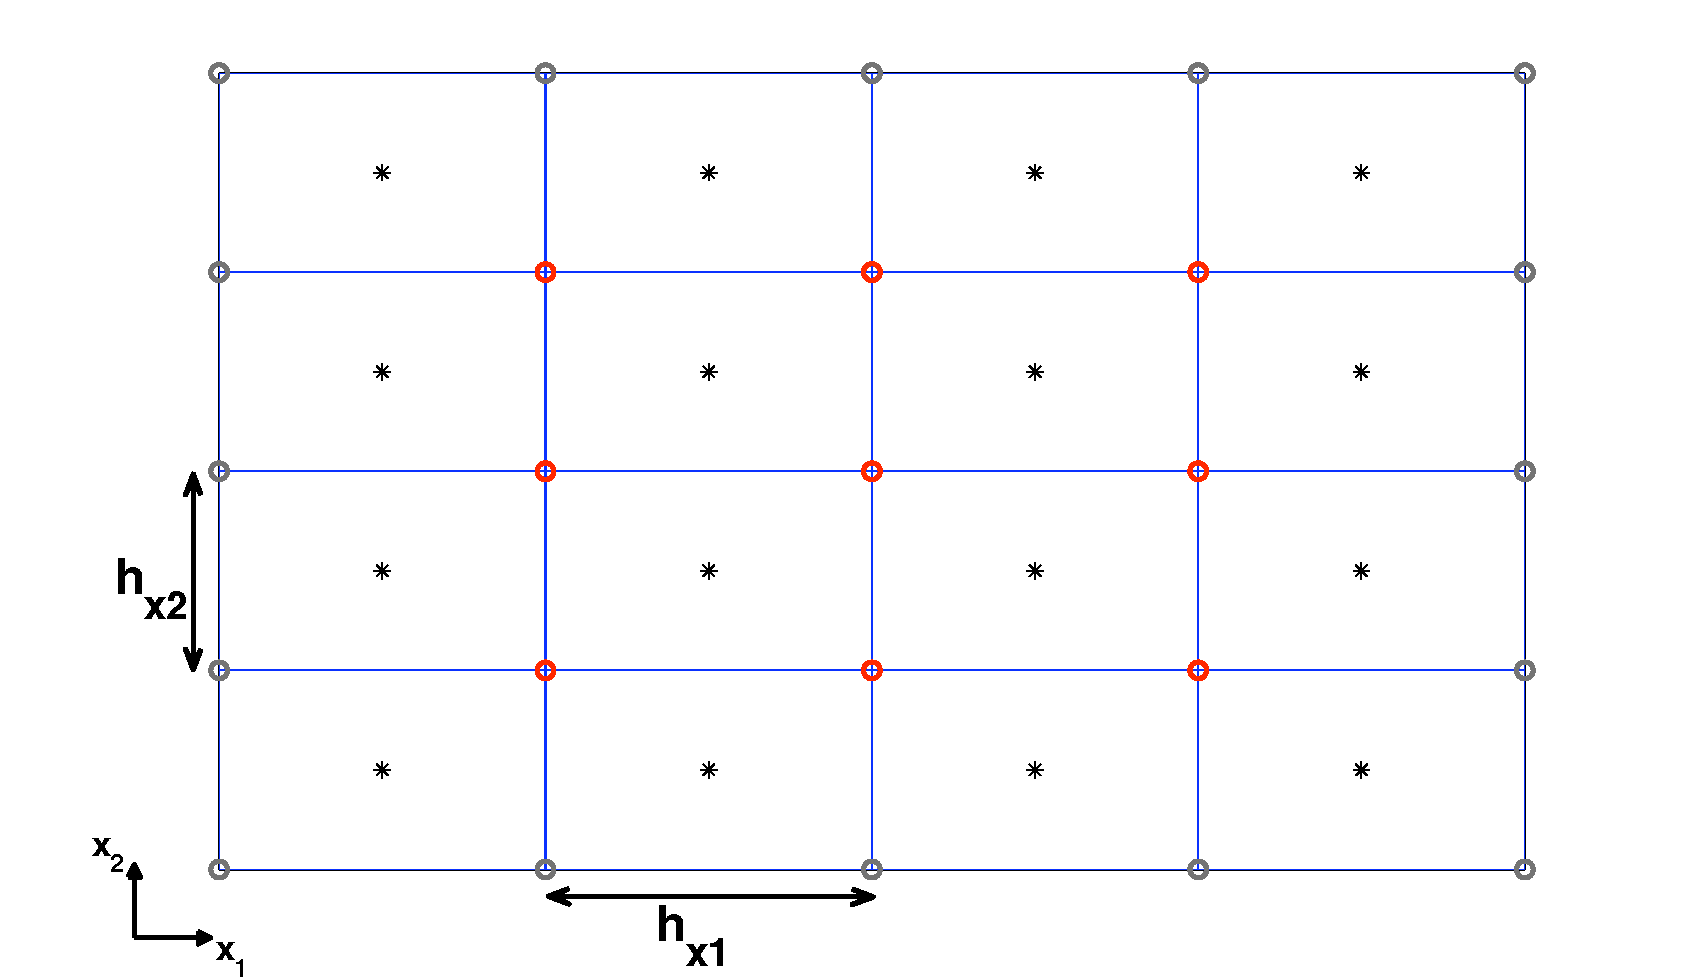
\includegraphics[width=10cm]{pics/q1p0/femsubdiv4.pdf}  
  \end{minipage}
  \caption{$Q_1P_0$ subdivision of a rectangular domain} 
\label{q1p0sub}
\end{figure}

The pressure is approximated by functions belonging to 
\begin{equation*}
 P_0(\Omega_h) = \bigl \{ q_h \in L^2(\Omega): q_h \bigl \vert _e= \const , \text{ for any } e\in \Omega_h \bigr \}
\end{equation*}
containing functions which are piecewise constant on every element $e$. Here $\Omega_h$ denotes the subdivided domain $\Omega$. For the given discretization, a function $q_h \in P_0$ is defined by the values for the $N^2$ cells of the $\Omega_h$. Accordingly the dimension of the pressure ansatz space $S_h=P_0(\Omega)$ is $N^2=:n_p$. A basis for $S_h$ is given by $\bigl \{ \psi_j \bigr \}_{j=1}^{n_p}$, where $\psi_j$ is the characteristic function for cell $e_j$.

\begin{rem}
 The Oseen equation and its approximations determine the pressure only up to a constant. To remove this degree of freedom from the pressure ansatz space one additional constraint is added, ensuring that $\int_\Omega q_h \inva x =0 $. Alternatively one can fix the pressure in one cell. Hence, at least for numerical computations, the dimension of $S_h$ is reduced to $N^2-1$.
\end{rem}


The velocity is approximated component-wise by means of scalar functions $v_h \in Q_1(\Omega_h) \subset H^1(\Omega)$ which are by definition bilinear on any element $e \in \Omega_h$ and continuous on $\Omega$. A function $v_h \in Q_1(\Omega_h)$ is uniquely defined by pregiven values in the corner of the cells, referred to as the velocity nodes $c_i$, $i=1,\dotsc,N^2$. 

A basis is given by 
\begin{equation*}
 \bigl \{ \eta_i\bigr \}_{i=1}^{N^2}, \quad \text{with } \eta_i(c_k) = \begin{cases} 
1& k=i\\ 
0& \text{else}
\end{cases} 
\end{equation*}
Demanding that $\eta_i$ is zero outside the adjoining cells, these basis functions are uniquely defined.

In the case of Dirichlet boundary conditions the values in the velocity nodes at the borders are fixed and thus one has $\dim Q_1(\Omega_h) = (N-1)^2$. For homogeneous boundary conditions the basis functions corresponding to the boundary are omitted and one has $Q_1(\Omega_h) \subset H_0^1(\Omega)$.

Then the vector valued space $\mathbf V_h$ can be defined via a separation of the basis functions for the $x_1$ and the $x_2$ component of the velocity:
\begin{equation} \label{canspli}
 \begin{split}
   \mathbf V_h &= \spann \bigl \{ \phi_1,\phi_2,\dotsc,\phi_{nv},\phi_{nv+1},\phi_{nv+2},\dotsc,\phi_{2nv} \bigr \}\\
&:=\spann \bigl \{ \begin{bmatrix} \eta_1 \\ 0 \end{bmatrix},\begin{bmatrix} \eta_2 \\ 0 \end{bmatrix},\dotsc,\begin{bmatrix} \eta_{nv} \\ 0 \end{bmatrix}, \begin{bmatrix} 0\\ \eta_1 \end{bmatrix},\begin{bmatrix} 0\\ \eta_2 \end{bmatrix},\dotsc,\begin{bmatrix} 0\\ \eta_{nv} \end{bmatrix} \bigr \}
 \end{split}
\end{equation}
with $n_v := (N-1)^2$. 

This splitting of the basis functions induces a splitting of the algebraic system defined for general finite element schemes in Section \ref{mfed}. Specifically, with $\mathbf v_h = [v_1,v_2,\dotsc,v_{n_v},v_{n_v+1},v_{n_v+2},\dotsc,v_{2n_v}]^T:= [\mathbf v_{h,x_1}^T \mathbf v_{h,x_2}^T]^T$, system \eqref{tralgoseen} reads
\begin{equation*}
	 \begin{bmatrix} M_1& 0 & 0\\ 0& M_1 & 0 \\ 0&0&0 \end{bmatrix} \frac{d}{dt}\begin{bmatrix} \mathbf v_{h,x_1}\\ \mathbf v_{h,x_2} \\ {\mathbf p}_h  \end{bmatrix}+ \begin{bmatrix} D_{x_1x_1}&D_{x_1x_2}& - B_{x_1}^T \\D_{x_2x_1}&D_{x_2x_2} & -B_{x_2}^T \\ B_{x_1} & B_{x_2} & 0 \end{bmatrix} \begin{bmatrix} \mathbf v_{h,x_1}\\ \mathbf v_{h,x_2} \\ {\mathbf p}_h  \end{bmatrix} = \begin{bmatrix} \mathbf f_{h,x_1}\\ \mathbf f_{h,x_2} \\ {\mathbf g}_h  \end{bmatrix} 
\end{equation*}
with the specific partioning for $D=A+N+W$ reading
\begin{equation*}
	 \begin{bmatrix} D_{x_1x_1}&D_{x_1x_2} \\D_{x_2x_1}&D_{x_2x_2} \end{bmatrix} =\begin{bmatrix} A_{1}&0 \\0&A_{1} \end{bmatrix} +\begin{bmatrix} N_{1}+W_{x_1x_1}&W_{x_1x_2} \\W_{x_2x_1}&N_1+W_{x_2x_2} \end{bmatrix} .
\end{equation*}

\subsection{The Coefficient Matrices for a 2D Domain}
Again the model problem of the previous section is considered, which enables a general presentation. For the extension of the presented formulas to nonuniform and nonrectangular grids the local specific geometry of the cells has to be adapted in the formulation.

As defined in Section \ref{mfed} the entries of the coefficient matrices are computed by integrating products of the $S_h$ and $\mathbf V_h$ basis functions and their derivatives over the whole domain $\Omega$. Since the set of cells $e_k$ represent a partitioning of $\Omega$ for the coefficients the following equality holds, exemplarily formulated for one entry of the \textit{vector-Laplacian} matrix $A$:
\begin{equation*}
 a_{ij} = \int _ \Omega \grad \phi_i : \grad \phi_j \inva x = \sum _{k=1} ^ {N^2} \int _{e_k} \grad \phi_i : \grad \phi_j \inva x
\end{equation*}
Supposing that $a_{ij}^{e_k}:=\int _{e_k} \grad \phi_i : \grad \phi_j \inva x$ define the entries of the element matrix $A^{e_k}$, one has 
\begin{equation*}
 A = \sum _{k=1} ^ {N^2}A^{e_k}
\end{equation*}
The same holds for the other coefficient matrices $M,B,N$ and $W$.

Since the basis functions have only a local support, for the computation of the element matrices only four velocity nodes and one pressure node have to be taken into account, as indicated in Figure \ref{q1p0el}.
\begin{figure}[htbp]
  \centering
  \begin{minipage}[b]{6 cm}
    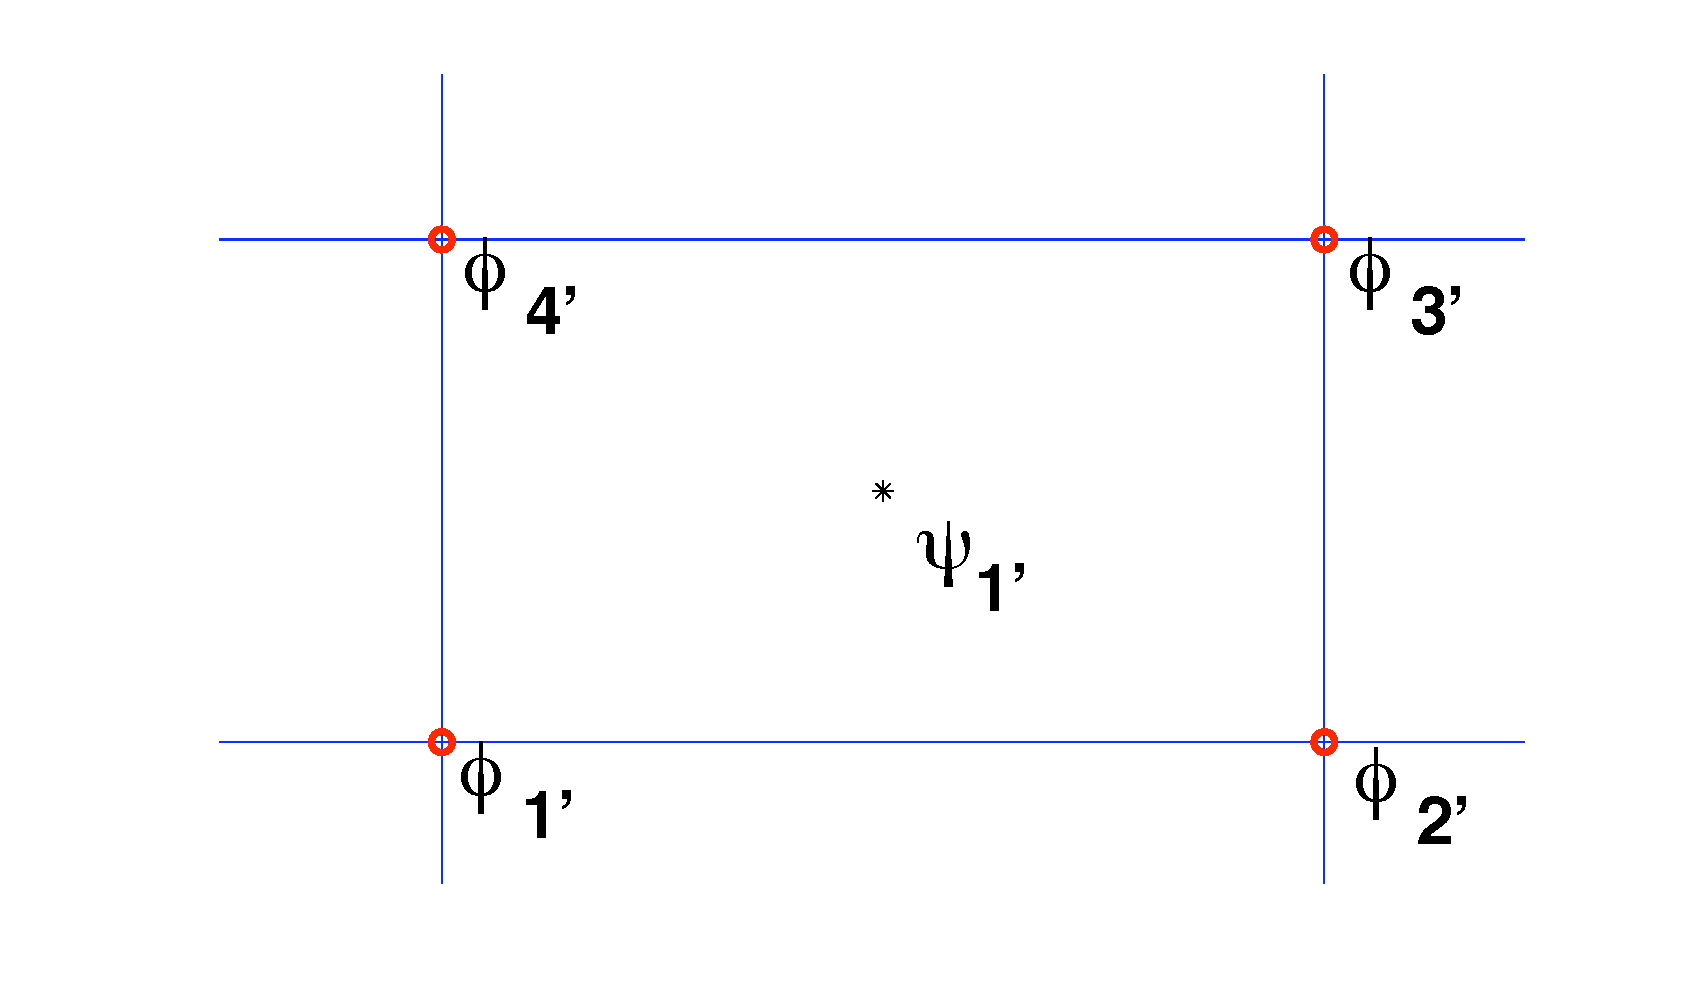
\includegraphics[width=6cm]{pics/q1p0/elemMa.pdf}  
  \end{minipage}
  \caption{One element $e'$ of a $Q_1P_0$ subdivision with its connected pressure and velocity nodes} 
\label{q1p0el}
\end{figure}

Suppose that the enumeration of the velocity basis functions given in Figure corresponds to a given element $e'$. Then $a_{ij}^{e'}=0$ unless $i,j\in\{1',2',3',4'\}$ yielding that $A_1^{e'} \in \mathbb R^{n_v\times n_v}$ has only $16$ nonzero elements. Since in this exemplary discretization all elements are of the same size, the element matrices only differ in the position of its entries, corresponding to the element specific enumeration $\{1',2',3',4'\}$. 

Also, the coefficient matrices $B_{x_1},B_{x_2}$ and $M_1$ can be displayed by one condensed element matrix. For the reassembling of the full matrices the local enumeration has to be reinterpreted. In the present $Q_1P_0$ discretization as displayed in Figure \ref{q1p0sub} one has 
for $i,j\in{1',2',3',4'}$ the mass matrix with $m^e_{ij} = \int _e \phi_i \phi_j \inva x$:
\begin{equation*}
 M^e_1 = \frac{h_{x_1}h_{x_2}}{36}\begin{bmatrix} 4&2&1&2 \\ 2&4&2&1 \\ 1&2&4&2 \\ 2&1&2&4 \end{bmatrix}
\end{equation*}
the vector-Laplacian matrix with $a^e_{ij} = \int _e \grad \phi_i : \grad \phi_j \inva x$ :
\begin{equation*}
 A^e_1 = \frac{h_{x_1}}{6h_{x_2}}\begin{bmatrix} \phantom{-}2& -2&-1&\phantom{-}1 \\-2&\phantom{-}2&\phantom{-}1&-1 \\ -1&\phantom{-}1&\phantom{-}2&-2 \\ \phantom{-}1&-1&-2&\phantom{-}2 \end{bmatrix}+\frac{h_{x_2}}{6h_{x_1}}\begin{bmatrix} \phantom{-}2&\phantom{-}1&-1&-2 \\\phantom{-}1&\phantom{-}2&-2&-1 \\ -1&-2&\phantom{-}2&\phantom{-}1 \\ -2&-1&\phantom{-}1&\phantom{-}2 \end{bmatrix}
\end{equation*}
the vector divergence matrices: $b^e_{x_1,1'i} = \int _e \psi_{1'} \frac{\partial \phi_i}{ \partial x_1}\inva x,~ b^e_{x_2,1'i} = \int _e \psi_{1'} \frac{\partial \phi_i}{ \partial x_2}\inva x $ :
\begin{equation*}
B_{x_1}^e = \frac{h_{x_1}}{2}\begin{bmatrix}\phantom{-} 1 \\ -1 \\-1 \\\phantom{-}1 \end{bmatrix} \andi B_{x_2}^e = \frac{h_{x_2}}{2}\begin{bmatrix} \phantom{-}1 \\ \phantom{-}1 \\-1 \\-1 \end{bmatrix}
\end{equation*}
and the vector gradient matrices $[B_{x_1}^e]^T$ and $[B_{x_2}^e]^T$
\begin{align*}
[B_{x_1}^e]^T &= \frac{h_{x_1}}{2}\begin{bmatrix} 1 & -1 &-1 & 1 \end{bmatrix} \\ \andi \quad \quad
[ B_{x_2}^e]^T &= \frac{h_{x_2}}{2}\begin{bmatrix} 1 & 1 & -1 & -1 \end{bmatrix}.
\end{align*}


For the convection matrix $N$ and $W$ this condensed form does not work in general. First, the restriction to four velocity basis functions has to be released, to capture the fact, that the convection matrices sum up both $x_1$ and $x_2$ component of the velocity. Second, the special chose of the reference velocity $\mathbf v_{\infty}$ affects the matrices.

For the case of homogeneous Dirichlet boundary conditions and $\mathbf v_\infty \in \mathbf V_h$, i.e.
\begin{align*}
 \mathbf v_\infty &= \sum _{i=1}^{n_v} v_{\infty,i}^{[1]}\phi_i+ \sum _{i=1}^{n_v} v_{\infty,i}^{[2]}\phi_{n_v+i} \\
&=\sum _{i=1}^{n_v} v_{\infty,i}^{[1]}\begin{bmatrix}  \eta_i \\  0 \end{bmatrix}+\sum _{i=1}^{n_v} v_{\infty,i}^{[2]}\begin{bmatrix}  0 \\  \eta_i \end{bmatrix}
\end{align*}
with the splitting of the coefficient vector $[\mathbf v_\infty] =\bigl [[\mathbf v_\infty ^{[1]}]^T  ~[\mathbf v_\infty ^{[2]}]^T \bigr ]^T $ and in accordance to \eqref{canspli}, a simplified formulation of $N+W$ can be derived. 

In the following derivations the domain $\Omega$ in the formulation of the integral is omitted: $\int \phi \inva x:= \int_\Omega \phi \inva x$. 

Thus, one has for the parts $N_1$ of the convection matrix $N$ corresponding to $c(\mathbf v_\infty \cdot \nabla)\mathbf v$
\begin{equation*}
 N_1= [n_{ij} ] , \quad \text {with  } n_{ij}=\smallint (\mathbf v_\infty \nabla) \eta_j \cdot \eta_i \inva x\quad \text{for  } i,j=1,\dotsc,n_v
\end{equation*}

For two-dimensional formulations $\nabla = [\partial_{x_1}~\partial_{x_2}]^T$ and for a given vector $\mathbf w \in \mathbb R^2$ a function $\eta = \eta(x_1,x_2)$ one has 
\begin{equation*}
 (\mathbf w \cdot \nabla) \eta = w_1\partial_{x_1}\eta + w_2\partial_{x_2}\eta \andi \partial_{x}(\cdot):=\frac{\partial}{\partial_{x}}(\cdot)
\end{equation*}

Using the canonical splitting of the basis and of $\mathbf v_\infty$ one obtains
\begin{equation*}
 n_{ij} = \smallint (\mathbf v_\infty  \nabla) \eta_j \cdot \eta_i\inva x = \sum_{k=1}^{n_v} v_{\infty,k}^{[1]}\ \smallint (\eta_k \partial_x \eta_j ) \eta_i\inva x+\sum_{k=1}^{n_v} v_{\infty,k}^{[2]}\ \smallint (\eta_k \partial_y \eta_j )\eta_i\inva x
\end{equation*}
and thus $N_1$ can be decoupled as $N_1=N_{x_1}^{[1]}+N_{x_2}^{[2]}$ with
\begin{equation*}
 \bigl [ N_{x_1}^{[1]} \bigr ]_{ij}=[\mathbf v_\infty ^{[1]}]^T \begin{bmatrix} \smallint \eta_1 \eta_i \partial_{x_1} \eta_j \inva x\\ \smallint \eta_2 \eta_i \partial_{x_1} \eta_j\inva x \\ \vdots \\ \smallint \eta_{n_v} \eta_i \partial_{x_1} \eta_j \inva x\end{bmatrix} \andi
\bigl [ N_{x_2}^{[2]} \bigr ]_{ij}=[\mathbf v_\infty ^{[2]}]^T\begin{bmatrix} \smallint \eta_{1} \eta_i \partial_{x_2} \eta_j \inva x\\ \smallint \eta_{2} \eta_i \partial_{x_2} \eta_j \inva x\\ \vdots \\ \smallint \eta_{n_v} \eta_i \partial_{x_2} \eta_j\inva x \end{bmatrix}
\end{equation*}
Analogously one can define $N_{x_2}^{[1]}$ and $N_{x_1}^{[2]}$ playing a role for the computation of the \textit{Newton derivative matrix} $W$. So let $W$ be the coefficient matrix corresponding to $c(\mathbf v \cdot \nabla)\mathbf v_\infty$, then, for the above splitting of $\mathbf v_\infty$, $W$ has the form
\begin{equation*}
 W= \begin{bmatrix} W_{x_1}^{[1]}& W_{x_1}^{[2]} \\ W_{x_2}^{[1]} & W_{x_2}^{[2]} \end{bmatrix} , \quad  \text{with  } [w_{x_k}^{[l]}]_{ij}=\smallint \partial_{x_k} \mathbf v_{\infty}^{[l]}  \eta_i \eta_j \inva x\quad \text{for  } i,j=1,\dotsc,n_v
\end{equation*}
and $k,l \in \{1,2\}$. Utilizing the homogeneous Dirichlet boundary conditions, a partial integration gives
\begin{align*}
\smallint \partial_{x_k} \mathbf v_{\infty}^{[l]}  \eta_i \eta_j \inva x=& -\smallint  \mathbf v_{\infty}^{[l]} \partial_{x_k} \bigl( \eta_i \eta_j \bigr)\inva x \\
=&-\smallint  \mathbf v_{\infty}^{[l]}  \eta_i \partial_{x_k} \eta_j\inva x -\smallint  \mathbf v_{\infty}^{[l]}  \eta_j \partial_{x_k} \eta_i\inva x
\end{align*}
Recalling that $\mathbf v_{\infty}^{[l]} = \sum _{i=1}^{n_v} v_{\infty,i}^{[l]} \eta_i\inva x$ one obtains for $i,j=1,\dotsc,n_v$ and $k,l \in \{1,2\}$
\begin{align}\label{estim}
 [w_{x_k}^{[l]}]_{ij} &= -[\mathbf v_\infty ^{[l]}]^T \begin{bmatrix} \smallint \eta_1 \eta_i \partial_{x_k} \eta_j\inva x \\ \smallint \eta_2 \eta_i \partial_{x_k} \eta_j \inva x\\ \vdots \\ \smallint \eta_{n_v} \eta_i \partial_{x_k} \eta_j \inva x\end{bmatrix}  - [\mathbf v_\infty ^{[l]}]^T \begin{bmatrix} \smallint \eta_1 \eta_j \partial_{x_k} \eta_i \inva x\\ \smallint \eta_2 \eta_j \partial_{x_k} \eta_i\inva x \\ \vdots \\ \smallint \eta_{n_v} \eta_j \partial_{x_k} \eta_i \inva x\end{bmatrix}\\
&= - (N_{x_k}^{[l]})_{ij}- (N_{x_k}^{[l]})_{ij}^T
\end{align}
Thus the following representation of the advective component is obtained:
\begin{equation*}
 N+W=\begin{bmatrix} \bigr[N_{x_2}^{[2]}\bigl]- \bigr[N_{x_1}^{[1]}\bigl]^T &- \bigr[N_{x_1}^{[2]}\bigl]- \bigr[N_{x_1}^{[2]}\bigl]^T\\ &\\ -\bigr [N_{x_2}^{[1]}\bigl]- \bigr[N_{x_2}^{[1]}\bigl]^T&\bigr[N_{x_1}^{[1]}\bigl]- \bigr[N_{x_2}^{[2]}\bigl]^T \end{bmatrix}
\end{equation*}

\begin{rem}\label{symd}
 The above formulas imply that the coefficients of the convection matrix $N+W$ are $\mathcal O(h_{x_1}+h_{x_2})$. This can be seen by the rough estimate of \eqref{estim}, giving e.g.
\begin{equation*}
 \abs{ \biggl [-\bigr [N_{x_1}^{[1]}\bigl]- \bigr[N_{x_2}^{[2]}\bigl]^T \biggr]_{ij}} \leq \max _l \abs{v_{\infty,l}}\left \{ \sum _{k=1}^{n_v}\abs{ \smallint \eta_k \eta_i \partial_{x_1} \eta_j\inva x} + \sum _{k=1}^{n_v}\abs{ \smallint \eta_k \eta_j \partial_{x_2} \eta_i\inva x}\right \}
\end{equation*}
If $i=j$ the the summations as e.g. $\sum _{k=1}^{n_v}\abs{ \smallint \eta_k \eta_i \partial_{x_2} \eta_j\inva x}$ have $9$ summands. If $i \neq j$ the the sum has $6,4$ or $0$ summands, as the support of the basis functions overlaps only for neighbouring velocity nodes. Further, having identified that
\begin{align*}
\max_{i,j,k=1,\dotsc,n_v} \abs{\smallint \eta_k \eta_i \partial_{x_1} \eta_j\inva x} &= \abs{\smallint \eta_l \eta_l  \partial_{x_1} \eta_l\inva x}= \frac{h_{x_2}}{3}, \\
\text{and}\quad \max_{i,j,k=1,\dotsc,n_v} \abs{\smallint \eta_k \eta_i \partial_{x_2} \eta_j\inva x} &= \abs{\smallint \eta_l \eta_l  \partial_{x_2} \eta_l\inva x}= \frac{h_{x_1}}{3} \quad \text{for any  }1\leq l \leq n_v
\end{align*}
one obtains
\begin{equation*}
 \abs{ \biggl [-\bigr [N_{x_1}^{[1]}\bigl]- \bigr[N_{x_2}^{[2]}\bigl]^T \biggr]_{ij}} \leq 6 (h_{x_1}+h_{x_2}) \max _l \abs{v_{\infty,l}}
\end{equation*}
and therefore, 
\begin{equation*}
 \abs{\bigl [ N+W \bigr ] _{ij}} \leq 6 (h_{x_1}+h_{x_2}) \max _l \abs{v_{\infty,l}} \quad \text{for }i,j=1,\dotsc,2n_v
\end{equation*}
since the above estimate holds equally for the remaining blocks in \eqref{estim}.
\end{rem}

\subsection{Pressure Modes and Stabilization}\label{pms}
One possible way to establish the discrete \textit{inf-sup condition} for a mixed finite element scheme, is to identify $\Omega_h$ as a patch of stable \textit{macroelements}. A stable macroelement is a cluster of elements, on which the local flow problem is well-posed, if the velocity is imposed everywhere on the boundary, c.f \cite{elma}. If a grid can be constructed by joining stable macroelements, then the \textit{inf-sup condition} is satisfied, see results in e.g. \cite{boni,sten}.

For the stability analysis of the $Q_1P_0$ discretization the $2\times2$-macroelement in Figure \ref{q1p0mac} is considered. The instability of a concrete patch does not imply the failure of the \textit{inf-sup condition}, the analysis of such macroelement, however, identifies the source of the well-known instability of the $Q_1P_0$ scheme, c.f. e.g. \cite{brhu,gunipe,sani}.

\begin{figure}[htbp]
  \centering
  \begin{minipage}[b]{6 cm}
    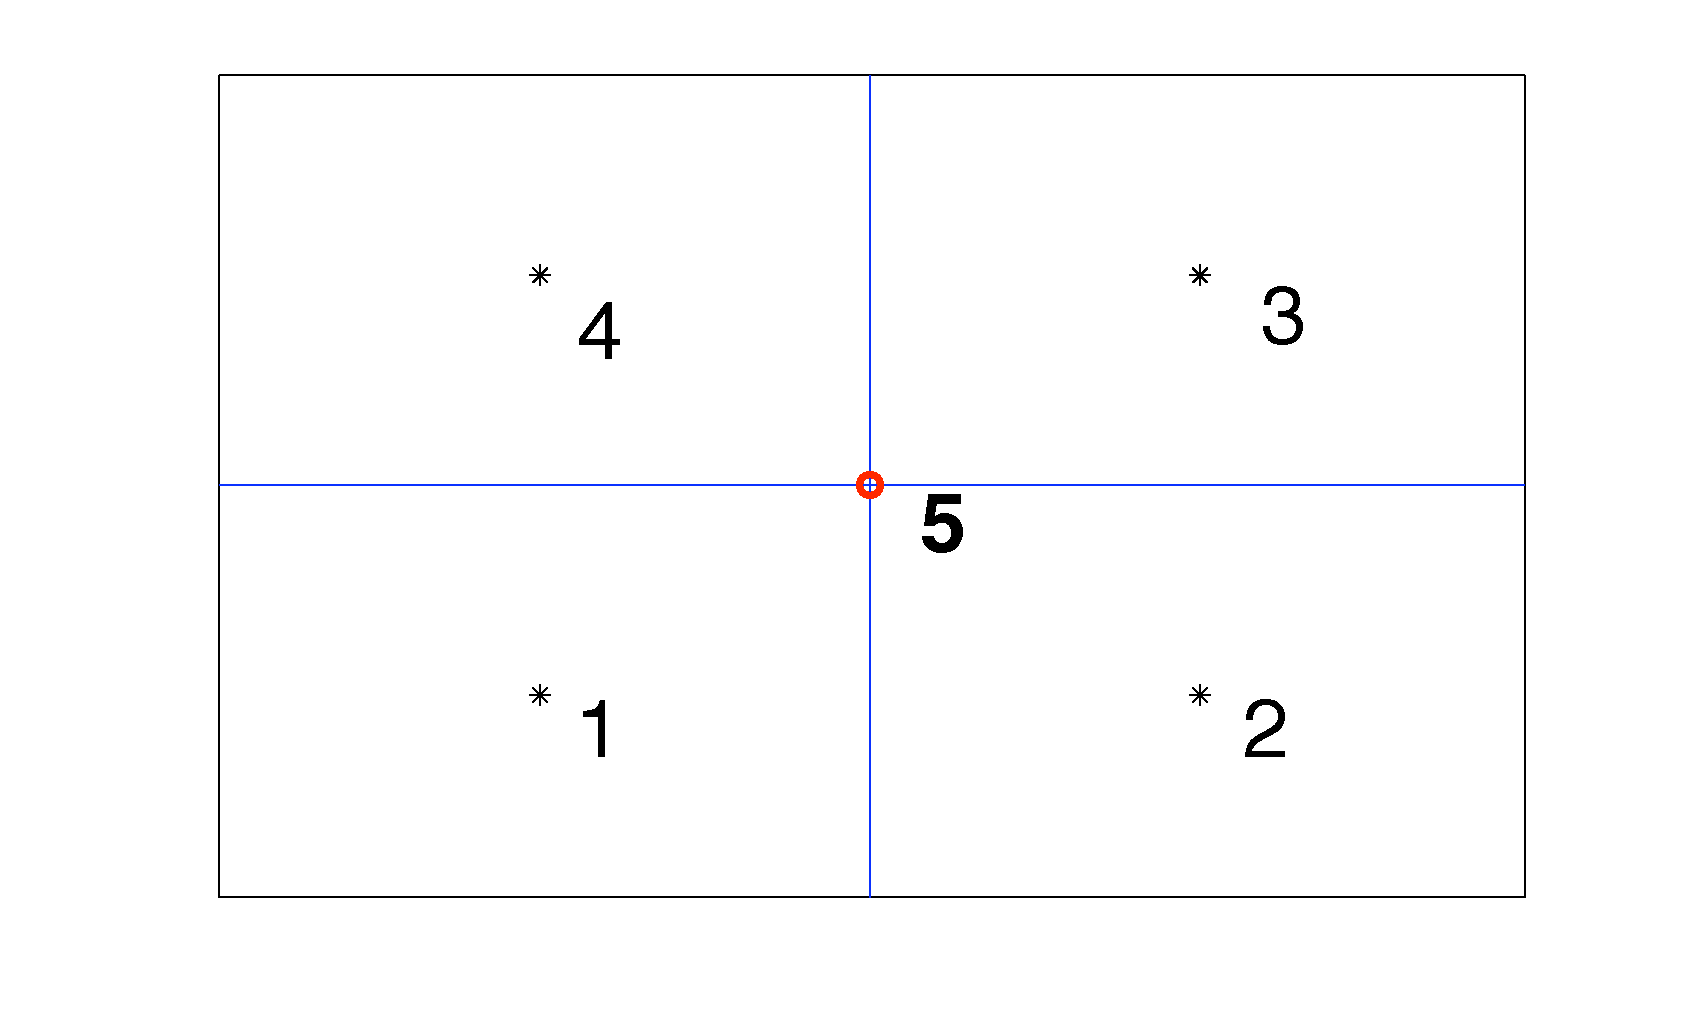
\includegraphics[width=6cm]{pics/q1p0/q1p0mac.pdf}  
  \end{minipage}
  \caption{$Q_1P_0$ macroelement} 
\label{q1p0mac}
\end{figure}

Posing a local Oseen problem on this macroelement with given velocity at the boundary gives the system 
\begin{equation}\label{macroseen}
 \begin{bmatrix} D & -B^T \\ B &  0 \end{bmatrix} \begin{bmatrix} \mathbf v_h \\ \mathbf p_h \end{bmatrix} = \begin{bmatrix} \mathbf
f_h \\ \mathbf g_h \end{bmatrix}
\end{equation}
with $D \in \mathbb R^{2\times2}$, which is supposed to be positive definite, and 
\begin{equation}\label{gradmac}
 B^T = \frac{1}{2} \begin{bmatrix} \phantom{-}h_{x_2}&-h_{x_2}&-h_{x_2}&\phantom{-}h_{x_1} \\ \phantom{-}h_{x_1}&\phantom{-}h_{x_1}&-h_{x_1}&-h_{x_1} \end{bmatrix}
\end{equation}
The pressure complement of system \eqref{macroseen} 
\begin{equation*}
 BD^{-1}B^T\mathbf p_h = BD^{-1}\mathbf f_h - \mathbf g_h
\end{equation*}
defines the pressure up to the nullspace of $B^T$. 

The nullspace of the gradient matrix for the considered macroelement, given by \eqref{gradmac}, contains the constant vector $\mathbf p_h = \mathbf 1:= [1~ 1~ 1 ~1]^T$, which is necessary since the freedom in the pressure has not been removed, and the \textit{checkerboard mode} $\mathbf p_h = \pm \mathbf 1$. 

It can be shown that the spurious pressure mode $\mathbf p_h = \pm \mathbf 1 $ is inherent in every rectangular $n\times m$ macroelement. Thus for a stable pressure approximation using $Q_1P_0$ elements it is necessary to remove the checkerboard mode on every macroelement. This is done by substituting the zero block in \eqref{macroseen} by a stabilization matrix Q, giving
\begin{equation*}
 \begin{bmatrix} D & -B^T \\ B &  \beta Q \end{bmatrix} \begin{bmatrix} \mathbf v_h \\ \mathbf p_h \end{bmatrix} = \begin{bmatrix} \mathbf
f_h \\ \mathbf g_h \end{bmatrix}
\end{equation*}
with a stabilization parameter $\beta$. Now the pressure complement reads
\begin{equation*}
 [BD^{-1}B^T+\beta Q]\mathbf p_h = BD^{-1}\mathbf f_h - \mathbf g_h
\end{equation*}
The stabilized system is well posed if the pressure matrix $S_\beta := [BD^{-1}B^T+\beta Q]$ is positive definite, suggesting that $Q$ should be positive semi-definite, and $\nulli S_\beta = \mathbf 1$. The latter condition ensures consistency, since the sought solution is not affected by the stabilization.

An example for a minimal stabilization, i.e. only the checkerboard mode is affected, is given by
\begin{equation*}
 Q_* = \begin{bmatrix}\phantom{-}1 &-1 &\phantom{-}1 &-1 \\-1 &\phantom{-}1 &-1 &\phantom{-}1 \\\phantom{-}1 &-1 &\phantom{-}1 &-1 \\-1 &\phantom{-}1 &-1 &\phantom{-}1 \end{bmatrix}
\end{equation*}
whereas the \textit{jump stabilization} matrix 
\begin{equation*}
 Q^* = h_{x_1}h_{x_2}\begin{bmatrix}\phantom{-}2 &-1 &\phantom{-}0 &-1 \\-1 &\phantom{-}2 &-1 &\phantom{-}0 \\\phantom{-}0 &-1 &\phantom{-}2 &-1 \\-1 &\phantom{-}0 &-1 &\phantom{-}2 \end{bmatrix}
\end{equation*}
affects every pressure mode not proportional to $\mathbf 1$. The derivation of $Q_*$ and $Q^*$ and strategies for the proper and optimal choice of the stabilization parameter $\beta$ is given in \cite[p. 237-243]{elma}. 

To obtain a global stable pressure approximation for the $Q_1P_0$ elements, the discretized domain $\Omega_h$ is subdivided into macroelements, which the stabilization is applied to. Having sorted the pressure coefficient by blocks, corresponding to the macroelement subdivision, the global stabilization matrix is a block diagonal matrix of the macroelement stabilization matrices.



\section[Time Integration of the Semidiscretized Equations]{Time Integration of the Semidiscretized Oseen Equations}\label{titso}
As stated above the Oseen system \eqref{soe1} represents a DAE of index two. The singularity of the coefficient matrix regarding the derivative of the state vector interdicts explicit time integration methods in general. Furthermore even implicit schemes both of low and high order do not guarantee reliable numerical results in advance. For a general discussion of these issues the reader is referred to \cite{mehr}, comprehensive and useful remarks with respect to flow problems are given in \cite[Ch. 3.16.1]{gre2}.

For the solution of the transient Oseen system one can adapt the most of the numerous solution methods for the Navier-Stokes equations. Many of the common solution methods can be interpreted as an \textit{index reduction} of the underlying DAE, cf. \cite{weic}. For example the various \textit{projection methods} are formulated by means of the \textit{pressure Poisson equation} (PPE) which is obtained by one derivation of the divergence-free constraint.


\subsection[Projection Algrorithms]{Projection Algorithms for Time-Dependent Flows}\label{paftn}

In particular in computational fluid dynamics projections methods have become very popular since Chorin's classical paper \cite{chorin} submitted in 1968. This is due to the relative simple implementation and the significant lowering of the computational effort coming with separate computation of the velocity and the pressure. This section addresses the derivation and working principle of projection methods for incompressible flow. For an overview of specific schemes and the analysis thereof the reader is referred to \cite{prohl}.

The formal derivation of a general \textit{projection algorithm} in the continuous case is briefly presented for the Navier-Stokes equations for a fluid with constant density in a well behaved domain $\Omega$ in a certain time interval. Leaving boundary and initial conditions aside, the system reads
\begin{align}
 \dot v - \frac{1}{Re} \Delta v +  (v \cdot \nabla) v+\nabla p =& f  \label{momeNS} \\
\nabla \cdot v =& 0  \label{kontNS}
\end{align}
which can be rewritten as 
\begin{equation}\label{spli}
 \dot v+\nabla p = S(v)  \andi \nabla \cdot v = 0
\end{equation}
where $S(v) := f+\frac{1}{Re} \Delta v -  (v \cdot \nabla) v$. Since \eqref{kontNS} applies for all times, it can be differentiated with respect to time and for a time independent domain one obtains $ \nabla \cdot \dot v  =0 $, i.e. also the acceleration $\dot v$ is divergence free. Furthermore one has $\nabla p$  is curl free as the gradient field of a scalar. 

Therefore, following Chorin \cite{chorin}, \eqref{spli} invoke the following interpretation. For a given velocity $v$ one can compute the vector $S(v)$ and project it onto the subspaces of both divergence free (here $\dot v = \mathscr P S(v)$) or curl free (here $\nabla p = \mathscr Q S(v)$) functions. 

The projectors $ \mathscr P$ and $ \mathscr Q $ are obtained as follows. Applying the divergence operator on \eqref{spli} eliminates the accelaration $\dot v$ and gives
\begin{equation} \label{ppe}
 \dive \grad p = \dive S(v)  
\end{equation}
a representation of the PPE. Since the Laplace operator $\dive \grad = \Delta$ is invertible, one can formally solve the PPE for the pressure to be given an expression for the pressure gradient
\begin{equation*}
 \grad p =\grad \Delta^{-1} \dive S(v)
\end{equation*}
and therefore for the operators $\mathscr Q = \grad  \Delta^{-1} \dive $ and $\mathscr P = I -\grad  \Delta^{-1} \dive $.

Simply put, in practice, a projection method in the continuum may work as follows. An approximated pressure gradient is used to compute by means of the momentum equation an \textit{intermediate velocity} $\tilde{v}$, which in general is not divergence free. Then $\tilde{v}$ is projected onto $v$ in the appropriate space of divergence free functions by solving the equations
\begin{align}
 v + \grad \phi &= \tilde v \label{fide} \\
\dive v &= 0
\end{align}
to obtain the velocity of the next timestep. The next iteration starts with guessing a new pressure gradient. Advanced schemes furthermore interpret $\phi$ as a pressure correction and update the pressure accordingly or reestablish it by means of the PPE \eqref{ppe}.

\begin{rem}
The use of the PPE includes the formulation $ \Delta p$ in the continuous case \eqref{ppe} and $-[BM^{-1}B^T]\mathbf p_h$ in the discrete analog. Since the pressure belongs to $L^2$ rather then to $H^1$ especially for low-order pressure approximations, e.g. $\mathbf p_h \in p1$, the use of $-[BM^{-1}B^T]\mathbf p_h$ requires additional reasoning. One approach is to interpret $-[BM^{-1}B^T]\mathbf p_h$ as an approximation to $ \Delta \mathbf p_h$ in regions of sufficiently smooth pressure and as \textit{an algebraic rearrangement of the equations} elsewhere, c.f. \cite[p.~642]{gre2}.
\end{rem}


\subsection{The Semidiscretized Linearized Case}

To derive the correponding propositions and operators for the semidiscretized (Oseen) case instead of \eqref{momeNS} and \eqref{kontNS} the system 
\begin{align}
 M\dot {\mathbf v}_h + D{\mathbf v}_h  -B^T {\mathbf p}_h &= {\mathbf f}_h   \label{momDi}\\
 B{\mathbf v}_h &= \mathbf g_h  \label{konDi}
\end{align}
deriving from a spatial discretization of the Oseen equations is considered in a time interval $[0,T]$. 

The underlying spatial discretization scheme can be chosen arbitrarily. Here the notation of a general mixed finite element scheme introduced in Section \ref{mfed} is used. Thus, $M \in \mathbb R ^{n_v \times n_v}$ denotes the mass matrix, $D=[A+N+W]\in \mathbb R ^{n_v \times n_v}$ contains the viscous and the convection terms, $B \in \mathbb R ^{n_p \times n_v}$ and $-B^T\in \mathbb R ^{n_v \times n_p}$ represent the discrete $ \dive $ and $\grad$ operators. 

The state variables $v$ and $p$ are now represented by vectors $\mathbf  v_h = \mathbf  v_h(t) \in \mathbb R^{n_v}$ and $\mathbf p_h=\mathbf p_h(t)\in \mathbb R^{n_p}$ containing the information on velocity and pressure, respectively. In contrast to the continuous case, the continuity equation is not automatically homogenous, since in the general case $\mathbf g_h$ possibly establishes the boundary conditions. 

Such as \eqref{momeNS}, \eqref{kontNS} imply \eqref{ppe}, also the discrete variants \eqref{momDi}, \eqref{konDi} can be rearranged:
\begin{equation*}
 \dot {\mathbf v}_h -  M^{-1} B^T \mathbf p    = M^{-1}( \mathbf f_h - A \mathbf v_h-[N+W]\mathbf v_h)
\end{equation*}
and imply the discrete Pressure Poisson equation
\begin{equation*}
 -[BM^{-1}B^T]\mathbf p_h=BM^{-1}(\mathbf f-A \mathbf v_h-[N+W]\mathbf v_h)-\dot {\mathbf g_h}
\end{equation*}
giving the formulas for the analogously to the continuous case defined projections 
\begin{equation*}
 \dot {\mathbf v}_h = \mathscr P_h M^{-1}(\mathbf f_h-A\mathbf v_h-[N+W]\mathbf v_h)-M^{-1} B^T  [BM^{-1}B^T]^{-1} \dot {\mathbf g}
\end{equation*}
and
\begin{equation*}
 -M^{-1}B^T\mathbf p_h = \mathscr Q_h M^{-1}(\mathbf f_h-A \mathbf v_h-[N+W]\mathbf v_h)-M^{-1} B^T  [BM^{-1}B^T]^{-1} \dot {\mathbf g}_h
\end{equation*}
with the projectors $\mathscr Q _h:=M^{-1} B^T  [BM^{-1}B^T]^{-1}B$ and $\mathscr P _h := I- \mathscr Q _h$.


\subsection{\textit{Projection2} for Semidiscretized Oseen}\label{p2fos}

The method used in this thesis is an adaption to the Oseen problem of the \textit{Projection2} algorithm as described in \citep{gre1,grc2}. First, the system coming from a spatial Q1P0 discretization of the Oseen equation is modified by inserting $MM_L^{-1}$ in front of the pressure term into the momentum equation:
\begin{equation*}
 M \dot{\mathbf v}_h + [A+N+W] \mathbf v_h - MM_L^{-1}B^T\mathbf  p_h =\mathbf f_h \label{momlm}
\end{equation*}
Here $M_L$ denotes the \textit{lumped mass} matrix, in which the mass represented by $M$ is concentrated on the diagonal. This slight modification causes only a small error, e.g. in \citep[p.~2.3.2a]{gre1} it is shown that the momentum equation is hardly effected since $MM_L^{-1}\mathbf v_h=\mathbf v_h+(h^2/6)\Delta \mathbf v_h + \mathcal O (h^4)$ for the discretization parameter $h$ and a sufficiently smooth function $\mathbf v_h$. Introducing this mixed mass matrices a compromise between the unaffordable computation of the dense $M^{-1}$ and the inconsistent and for convection dominated flows often inaccurate use of the diagonal lumped mass matrix. The motivation of this compromise becomes evident, when \eqref{momlm} is rewritten as
\begin{equation*}
  \dot{\mathbf v}_h + M^{-1}[A+N+W]\mathbf  v_h - M_L^{-1}B^T \mathbf p_h =M^{-1}\mathbf f_h,
\end{equation*}
which shows that for the calculation of $\dot {\mathbf v}_h$ the convection terms are approximated globally while only the pressure contributes locally. Another backbone of the \textit{Projection2} algorithm is the pressure update, which is closely related to the question how the auxiliary function $\phi$ in \eqref{fide} can be interpreted in terms of the pressure correction. Assuming sufficient smoothness in the variables and compatible boundary conditions one can derive 
\begin{equation*}
 \phi(T) = \frac{T^2}{2} \dot p_0 + \mathcal O (T^3)
\end{equation*}
holds as shown in  \cite[p. 595]{grea}, which is used in the algorithm to model 
\begin{equation}\label{phip}
 \grad \mathbf \phi(\tau)  \approx -\frac{\tau }{2}  B^T ( \mathbf p_h -\mathbf  p_{0,h})  
\end{equation}
and simultaneously defines the pressure update. 

Thus, knowing $\mathbf p_h^n$ and $\mathbf v_h^n$ satisfying the discretized momentum and possibly stabilized continuum equation at timestep $n$, \textit{Projection2} defines the steps to march a time distance of length $\tau$ as described in Algorithm \ref{alg:GS}.

\stepcounter{algorithm}
\stepcounter{algorithm}

\begin{algorithm}
\caption{\textit{Projection2} for Stabilized Oseen}
\label{alg:GS}

\begin{description}
 \item[Step 1] Solve
\begin{equation*}
 M\frac{(\tilde {\mathbf v}_h^{n+1}-\mathbf v_h^n)}{\tau}+A\tilde {\mathbf v}_h^{n+1}+[N+W]\mathbf v_h^n-MM_L^{-1}B^T\mathbf p_h^n=\mathbf f_h^n
\end{equation*}
for the intermediate velocity $\tilde {\mathbf v}_h^{n+1}$
\item[Step 2] Project $\tilde {\mathbf v}_h^{n+1}$ onto the function $\mathbf v_h^{n+1}$ satisfying the divergence equation via solving the equation system (c.f. \eqref{fide});
\begin{align}\label{spp}
 M_L \mathbf v_h^{n+1} -B^T \mathbf{ \phi} &= M_L \tilde {\mathbf v}_h^{n+1} \\
 B \mathbf v_h^{n+1} + \beta Q \phi &= \mathbf g_h^{n+1} \label{betq}
\end{align}
\item[Step 3]
Update the pressure according to \eqref{phip};
\begin{equation*}
 \mathbf p_h^{n+1} = \mathbf p_h^n+\frac{2}{\tau}\phi
\end{equation*}
Reset $n$ and go to Step 1!
 \end{description}
\end{algorithm}

 For clearness reasons the Algorithm is presented using simple Euler integration to solve for the \textit{intermediate velocity} $\tilde v$. As advised in \citep[p.~852]{gre1} for the actual implementation higher order schemes like trapezoidal rule or Adam-Bashforth 2 should be used for the integration of the momentum equation.

A detailed description of the algorithm and further helpful and constructive remarks can be found in \citep{gre1,grea,grc2}. 

\chapter{Numerical Tests}\label{numte}

The general setup is a driven cavity flow in a two-dimensional square domain, subject to a distributed control and observed via outputs, extracted from the velocity field. The behaviour of the fluid is modeled by the Oseen equation, spatially discretized by $Q_1P_0$ finite elements as introduced in Section \ref{q1p0}. The resulting, still time dependent, linear differential algebraic equation are numerically integrated using the \textit{Projection2} algorithm explained above. 

All numerical tests listed below were carried out in \textsc{Matlab} \cite{matl}. The open source toolbox IFISS \cite{ifis} served as the basis for several routines especially for the spatial discretization and the visualisation of the flow field. 

\section{The Driven Cavity Flow Testproblem}

The driven cavity flow problem is one of the classical test problems for \textit{computational fluid dynamics} (CFD) codes. Driven cavity flow means the movement and rotation of a fluid in a closed domain, forced by the impulse transferred to the fluid as e.g. via one constantly moving boundary. In nature this flow pattern can be observed in cavities on surfaces, which are tagentially attacked by a moving fluid, as e.g. an open roof of a driving car or the inter car gaps of a moving train.

The driven cavity in a two-dimensional square with one constantly moving boundary is supposed to be stable, e.g. it possesses a unique steady solution which is robust against small perturbations, up to a Reynolds number in the vicinity of $10^4$, c.f. the contribution of Qu\'er\'e et al. to \cite[p.~211]{dcp}. However several numerical investigations detected critical Reynolds numbers for the transition to the unsteady behaviour, that were below $10^3$, c.f. e.g. \cite{dingka,tdo} and the references therein. As a rule, the results presented for the driven cavity by different authors coincide quite well up to $Re = 1000$. For higher Reynolds numbers the predicted values for e.g. the critical Reynolds number, marking the first occurrence of multiple solutions, differ with the use of different discretization schemes on different grids, see \cite{brhesa,erco} for a summary of results. A concise description of the various regimes of the driven cavity flow for different Reynolds numbers is given in \cite{shde}.


\subsection{The Setup}

The domain considered throughout these investigations is a two-dimensional square represented by the computational domain $\Omega = \{ (x_1,x_2) \in (-1,1)^2 \}$. The driven cavity flow is defined by the boundary conditions imposing that the velocity is zero everywhere on the boundary except from $x_1$-component on the upper lid. There one sets $v_{x_1} = 1$, see Figure \ref{drivcav}.

\begin{figure}[htbp]
\begin{center}
 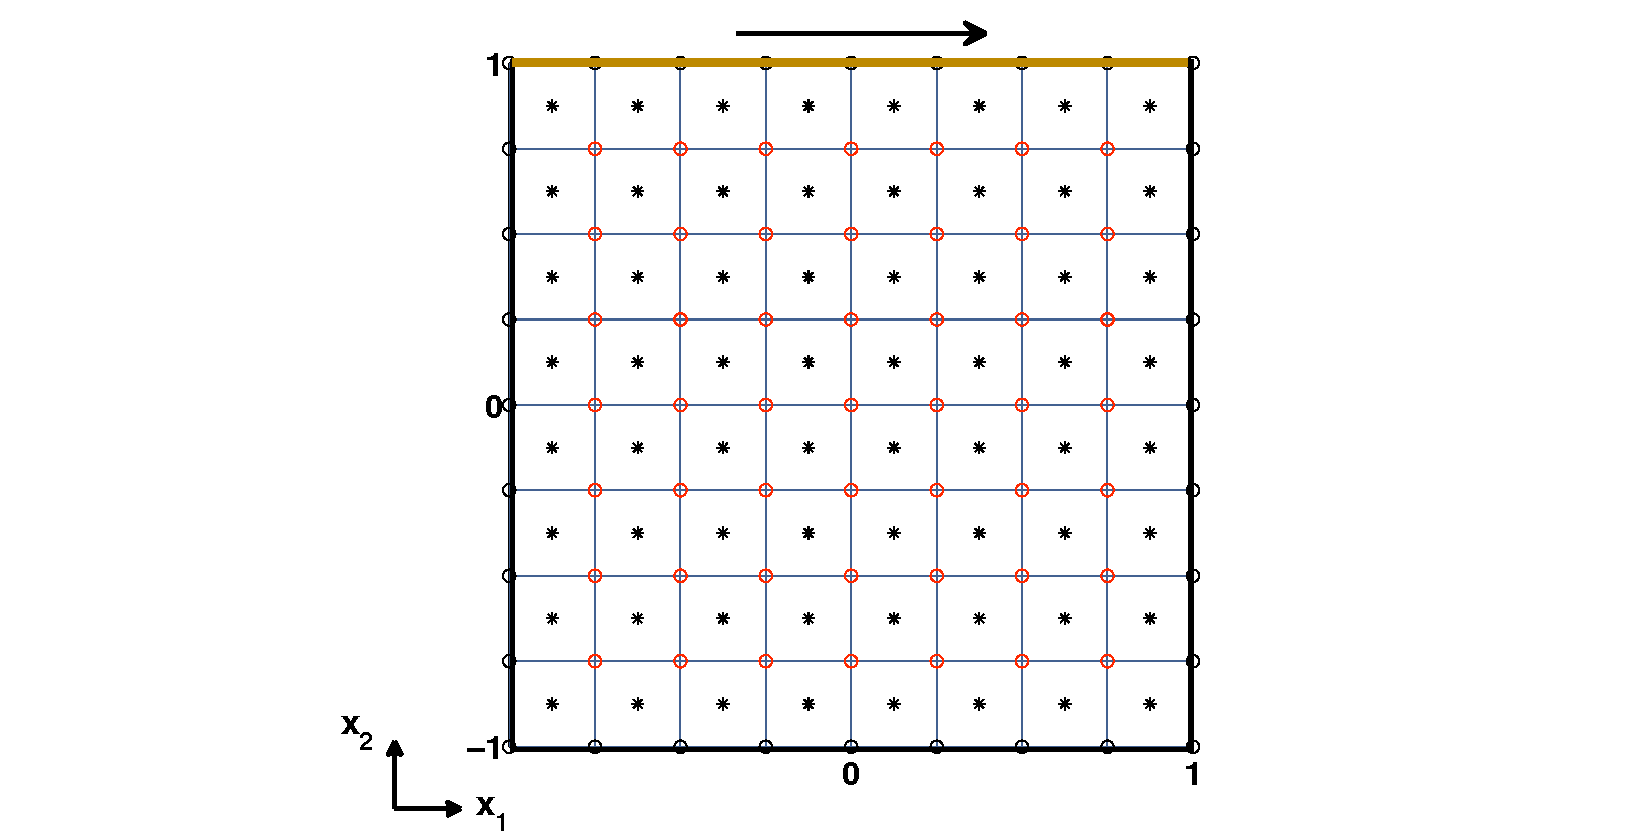
\includegraphics[width=10cm]{pics/q1p0/drivcav.pdf}
 \caption{An exemplary $Q_1P_0$ discretization of the domain $[-1,1]^2$ square with $h_{x_1}=h_{x_2}=:h$. The moving upper lid is modeled by imposing $v_{x_1} = 1$ for $ x_2 = 1$.}
 \label{drivcav}
\end{center}
\end{figure}

Supposing there is no external force acting on the fluid, for a suitably chosen reference solution $v_\infty$ the considered infinite dimensional Oseen system reads
\begin{subequations}\label{drivcavos}
\begin{align}
  v_t +  (v_\infty \cdot \nabla) v+(v \cdot \nabla) v_\infty+\nabla p - \frac{1}{Re} \triangle v =&  (v_\infty \cdot \nabla) v_\infty  \\
\nabla \cdot v =& 0 \\
v\lvert _{t=0} =  v_0  \quad \quad \quad\quad \quad \quad\quad \quad \quad\quad ~~ \\
v\lvert_{\partial \Omega} = \begin{cases}[1~0 ]^T&\text{if } x_2 = 1 \\ [0~ 0]^T &\text{elsewhere on $\partial \Omega$} \end{cases}
\end{align}
\end{subequations}
defining the pressure $p:[0,T] \times [-1,1]^2 \rightarrow \mathbb R$ and the velocity
\begin{equation*}
 v:[0,T] \times [-1,1]^2 \rightarrow \mathbb R ^2:v(t;x_1,x_2)=\begin{bmatrix} v_{x_1} \\ v_{x_2} \end{bmatrix}
\end{equation*}
for a given initial velocity $v_0$.

To keep the linearization error small and since the scope of this investigation is closed-loop control that acts locally in time, $T=0.1$ was chosen. 

This nondimensional formulation is parameterized by the Reynolds number defined by the product of the actual velocity of the lid with the actual side length of the domain. Hence, increasing the Reynolds number, as illustrated in Figure \ref{drivcavre}, means an increase of the lid velocity or the domain in the physical model. Throughout this numerical simulation the Reynolds number was set to $Re = 1333$, which, if air is taken as the flow medium, corresponds to a cavity of size $0.1m$ and a lid velocity of $0.2 m/s$. 

\begin{figure}[htbp]
  \centering
  \begin{minipage}[b]{3.9 cm}
    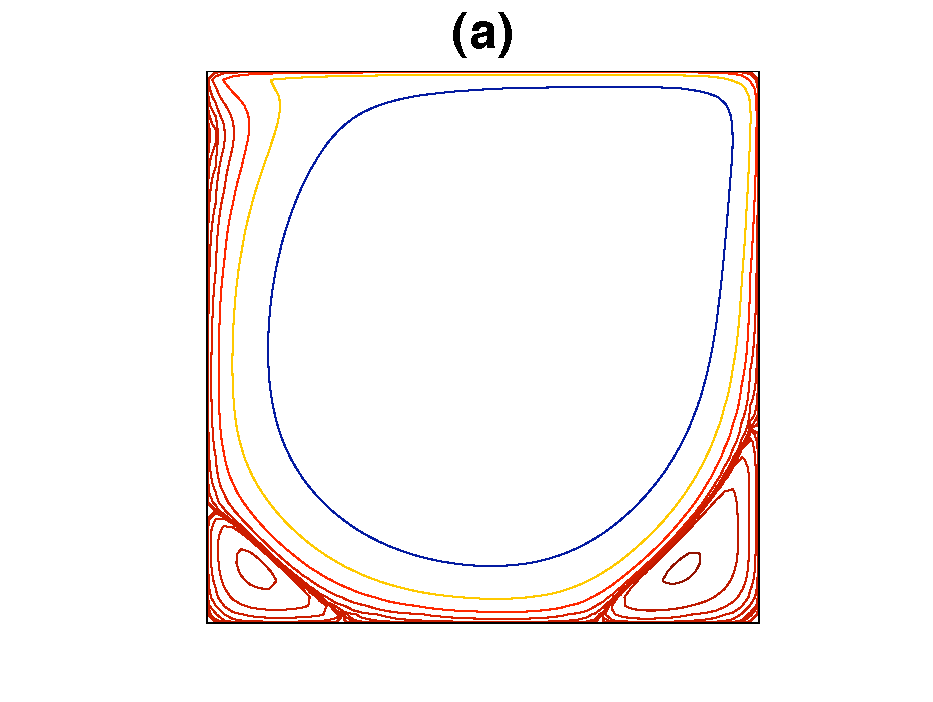
\includegraphics[width=3.9cm]{pics/numex/drivcavRe1333.pdf}  
  \end{minipage}
  \begin{minipage}[b]{3.9 cm}
    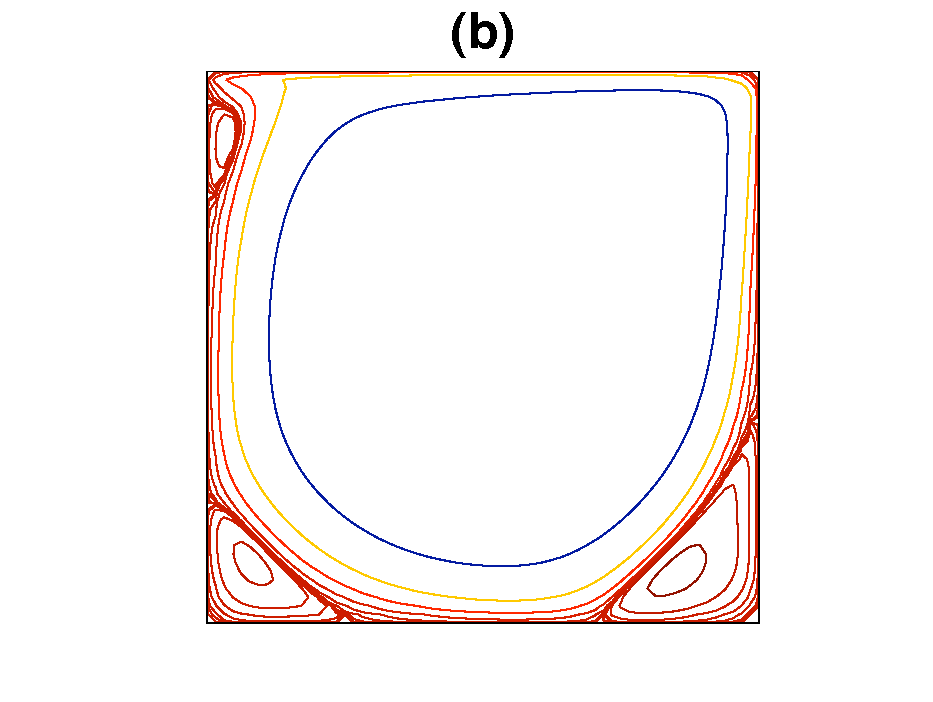
\includegraphics[width=3.9cm]{pics/numex/drivcavRe2333s.pdf}  
  \end{minipage}
  \begin{minipage}[b]{3.9 cm}
    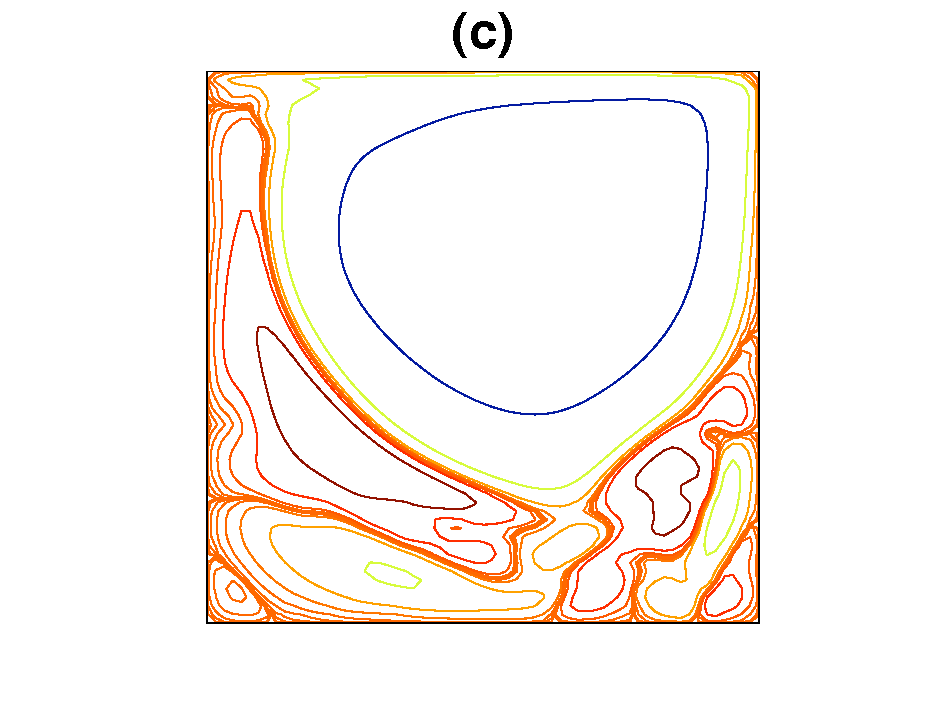
\includegraphics[width=3.9cm]{pics/numex/drivcavRe3333.pdf}  
  \end{minipage}
  \caption{Streamline plot of steady-state solutions of the driven cavity with variable Reynolds number on a $32\times32$ $Q_1P_0$ grid. (a): $Re = 1333$, (b): $Re = 2333$, (c): $Re = 3333$,}
  \label{drivcavre}
\end{figure}

The DAE form was obtained by a stabilized $Q_1P_0$ spatial discretization of the above system, using the subdivided domain $\Omega_h$ consisting of $32 \times 32$ equal squares. Recalling the definitions in Section \ref{q1p0} and the Dirichlet boundary conditions, one has $n_v=31^2$ and $n_p = 32^2-1$. 

For the pressure stabilization the pressure jump stabilization matrix $Q^*$ (see Section \ref{pms}) with the stabilization parameter $\beta = 1/4$ as suggested in \cite[p. 241]{elma} was used. As the reference velocity $\mathbf v_\infty$ the $Q_1P_0$ solution of the corresponding steady-state Navier-Stokes equations was taken, approximately computed by the built-in routines in \cite{ifis}.

Defining the coefficient matrices and the right-hand side in line with Section \ref{q1p0} the $Q_1P_0$ approximation of \eqref{drivcavos} reads: 

\begin{prob}

Find coefficient vectors $\mathbf v_h(t) \in \mathbb R^{2n_v}$ and $\mathbf p_h(t) \in \mathbb R^{n_p}$ corresponding to $\mathbf v_h(t) \in Q_1(\Omega_h)$ and $p_h(t) \in P_0(\Omega_h)$, respectively, so that
\begin{align}\label{algos1}
	\begin{bmatrix} M& 0 \\ 0& 0 \end{bmatrix} \frac{d}{dt} {\begin{bmatrix} \mathbf v_h \\ \mathbf p_h  \end{bmatrix}} + \begin{bmatrix} D& -B^T \\  B& \frac{1}{4}Q^* \end{bmatrix} \begin{bmatrix} \mathbf v_h \\ \mathbf p_h  \end{bmatrix} &= \begin{bmatrix} \mathbf f_h \\ \mathbf g_h \end{bmatrix} \\
\intertext{holds in $(0,T]$, and}
\mathbf v_h(0) = \mathbf v_{h,0}&.
\end{align}
\end{prob}

For the investigation of the i/o map, the initial condition was chosen as $\mathbf v_{h,0} = \mathbf v_\infty$.

These still time dependent equations, were numerically integrated using the \textit{Projection2} algorithm with \textit{backward Euler} as described in Section \ref{p2fos}.

\subsection{Convergence of \textit{Projection2}}
For a significant investigation of the discrete i/o behaviour, further possible computation errors have to be kept down. On the one hand, the error caused by the numerical integration of the state equations has to be reduced to an acceptable and affordable minimum. To investigate the error caused by the integration using the \textit{Projection2} algorithm, system \eqref{algos1} was integrated with the intial conditions $\mathbf v_0=0$ with different timestep sizes $\tau$. Then  the error in the velocity $\epsilon_v:=\norm{\mathbf v_h(0.1) - \mathbf v_h^*(0.1)}_0$ was measured in the $L^2$-norm on $Q_1(\Omega_h)$, where $v_h^*(0.1)$ denotes the solution of the system approximated with a very fine time resolution $\tau = 10^{-7}$.

The evaluation of $\epsilon_v$ versus various timesteps $\tau$, given in Figure \ref{p2conv}, showed a linear behaviour of the error, which is in line with \cite[p.~634]{grc2}.

\begin{figure}[htbp]
\begin{center}
 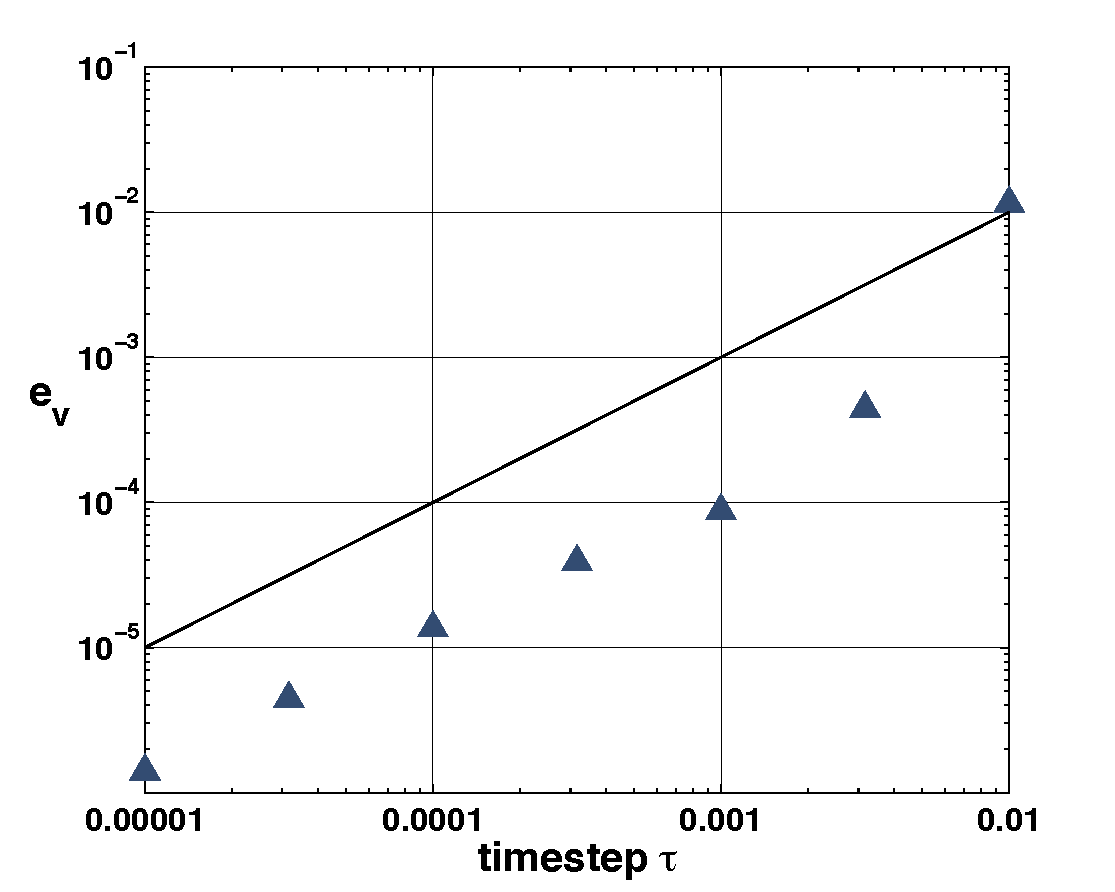
\includegraphics[width=9cm]{pics/numex/convp2.pdf}
 \caption{Behaviour of the numerical \textit{Projection2} integration error in the velocity. The diagonal denotes the slope of linear convergence}
 \label{p2conv}
\end{center}
\end{figure}

\section{Distributed Control of the Driven Cavity}\label{dcdc}

In order to control the flow in the driven cavity, an input term has to be added to the spatially discretized Oseen equations. Also an output has to be defined, along with suitable domains and function spaces.

As the domain of control $\Sigma := [-0.5,0.5] \times [-0.7,-0.5]  $, and as the domain of observation $\Theta := [-0.1,0.1] \times [0,0.6]$  were chosen, c.f. Figure \ref{pdco}.

\begin{figure}[htbp]
\begin{center}
 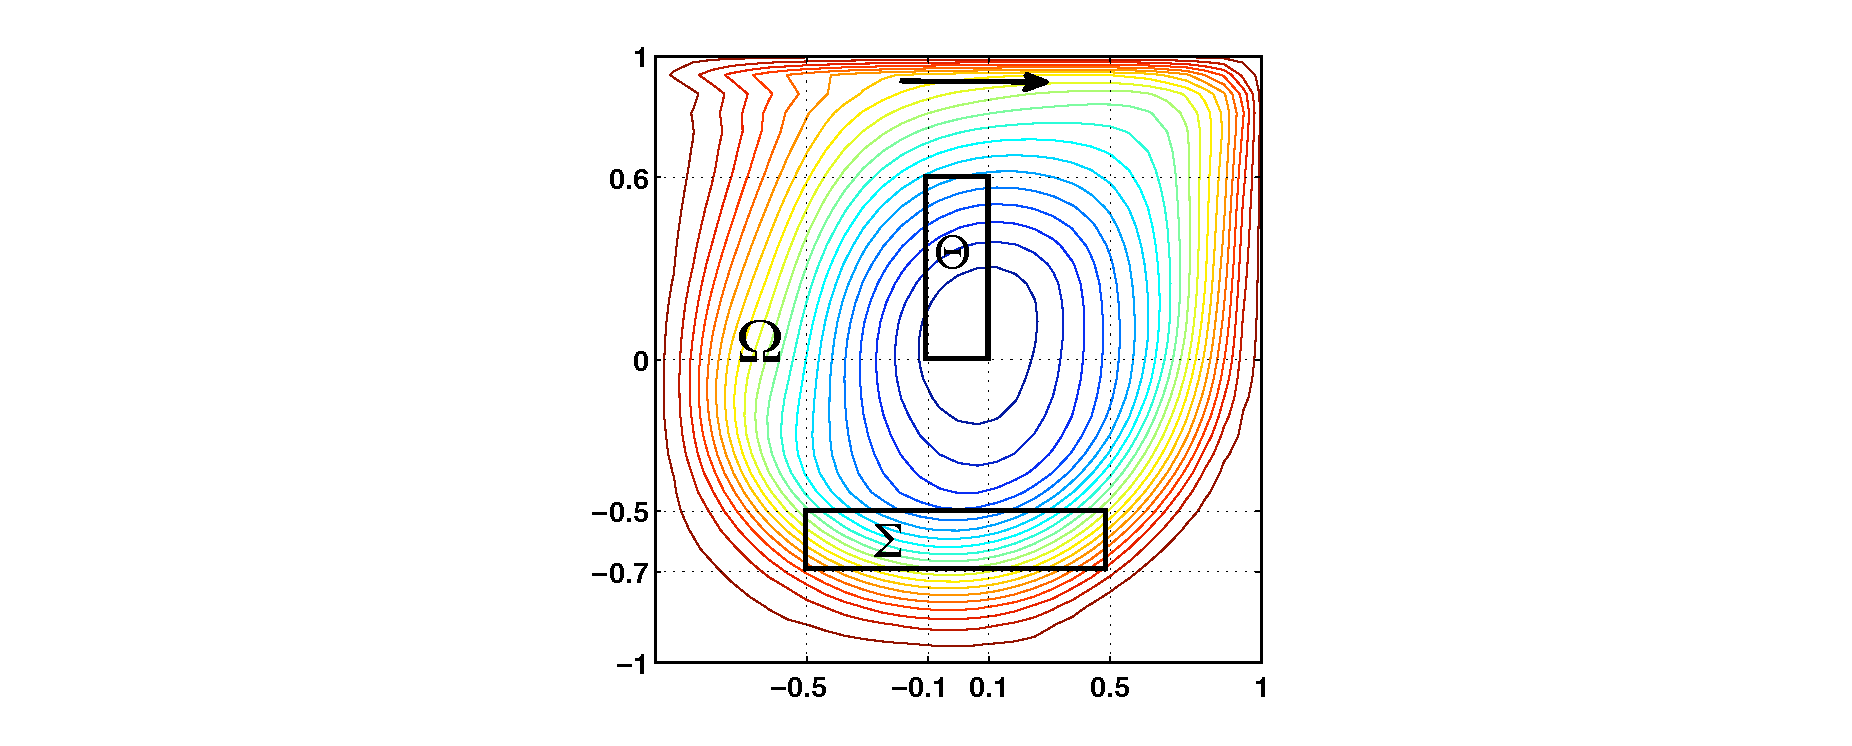
\includegraphics[width=8cm]{pics/domains.pdf}
 \caption{Computational domain $\Omega$ and areas of control $\Sigma$ and observation $\Theta$}
 \label{pdco}
\end{center}
\end{figure}

In view of influencing the $x_1$- and the $x_2$-components of the right-hand side, $U = Q_1(\Omega_h)$ was chosen as the state space of input functions. In order to define $U_h \subset U$ let $\mathfrak N_\Sigma$ denote the set of $n_\Sigma \times m_\Sigma$ velocity nodes $\mathfrak n$ of the $Q_1$ discretization, that are located in the inner of $\Sigma$. Renumbering the nodes $\mathfrak n \mapsto \mathfrak n_j^i$, with $i\in{1,\dotsc,n_\Sigma}$ representing its $x_1$-coordinate and $j\in{1,\dotsc,m_\Sigma}$ its $x_2$-coordinate as illustrated in Figure \ref{numvelnod} one has
\begin{equation*}
 \mathfrak N_\Sigma = \bigl \{ \mathfrak n_j^i: i\in{1,\dotsc,n_\Sigma},j\in{1,\dotsc,m_\Sigma} \bigr \}
\end{equation*}
Let $\eta_j^i$ be the nodal $Q_1(\Omega_h)$ basis function associated with node $\mathfrak n_j^i$, then one can define 
\begin{align*}
 U_h := &\spann \bigl \{ \mu_{1}, \dotsc ,\mu_{n_\Sigma}, \mu_{n_\Sigma +1}, \dotsc , \mu_{2n_\Sigma}  \bigr \}\\
&:=\spann \bigl \{ \begin{bmatrix} \xi^1 \\ 0 \end{bmatrix}, \dotsc , \begin{bmatrix} \xi^{n_\Sigma} \\ 0 \end{bmatrix},\begin{bmatrix} 0 \\ \xi^1 \end{bmatrix}, \dotsc , \begin{bmatrix} 0 \\ \xi^{n_\Sigma} \end{bmatrix} \bigr \}
\end{align*}
with $ \xi^i := \sum _{j=1}^{m_\Sigma}\eta_j^i $ for $i=1,\dotsc,n_\Sigma$. The dimension of $U_h$ is $2n_\Sigma =: p$.

In words, $U_h$ contains functions $\mathbf u_h \in Q_1(\Omega_h)$ with $\mathbf u_h=0$ on elements that don't intersect with $\Sigma$ and $\mathbf u_h = \const $ in $x_2$-direction on elements belonging to the inner of $\Sigma$. The latter condition implies that $\mathbf u_h \in U_h$ has no additional degrees of freedom in $x_2$-direction. 

\begin{figure}[htbp]
\begin{center}
 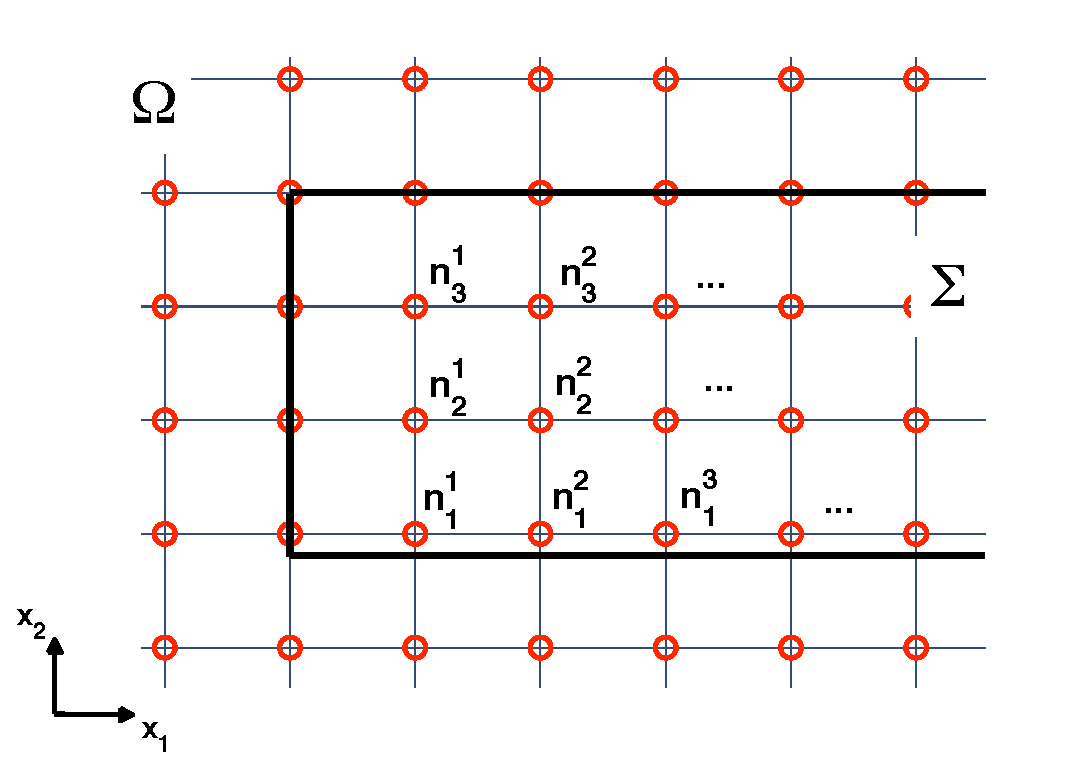
\includegraphics[width=8cm]{pics/numex/numvelnod.pdf}
 \caption{Enumeration of the velocity nodes $\mathfrak n$ belonging to the inner of $\Sigma$}
 \label{numvelnod}
\end{center}
\end{figure}

Thus for $t\in [0,T]$ one can define $\mathbf u_h(t) \in U_h$ via
\begin{equation*}
 \mathbf u_h(t) = \sum _{i=1}^{n_\Sigma}u_{x_1}^i(t)\mu_i+ \sum _{i=1}^{n_\Sigma}u_{x_2}^i(t)\mu_{n_\Sigma+i}
\end{equation*}
with functions $u^i_{x_1},u^i_{x_2}\in L^2(0,T)$, defining for $t\in [0,T]$ the $x_1$- and $x_2$-component of the signal at the nodes $\mathfrak n_1^i, \dotsc, \mathfrak n_{m_\Sigma}^i$, with $i=1,\dotsc,n_\Sigma$.

Let $\mathcal R_{k_1} := \spann \bigl \{ \varphi_1, \dotsc ,\varphi_r \bigr \} \subset  L^2(0,T)$ be a finite dimensional subspace of dimension $r$, then the discrete input signal space can be defined via
\begin{equation*}
 \mathcal U_{h,k_1} := \spann \bigl \{ \mu_i\varphi_j: i=1,\dotsc,p, ~j=1, \dotsc ,r \bigr \}
\end{equation*}
In the following analysis the function $\mathbf u_{hk_1} \in \mathcal U_{hk_1} $ and its coefficient vector $\mathbf u_{hk_1} \in \mathbb R^{p\cdot r}$ are used without special distinction. The same holds for $\mathbf u_{hk_1}(t) \in U_h$ and the corresponding vector $\mathbf u_{hk_1}(t)$.

Since $U_h \subset U = Q_1(\Omega_h)$ one has $\mathbf u_{hk_1}(t) \in Q_1(\Omega_h)$ and its coefficient vector $\mathbf u_{hk_1}(t) \in \mathbb R^{2n_v}$ can be filled up with zeros to become $\tilde {\mathbf u}_{hk_1}(t) \in \mathbb R^p$, representing $\mathbf u_{hk_1}(t)$ in $Q_1(\Omega_h)$. 

Having chosen the input operator $\mathcal B$ as the identity the control $\mathbf u_{hk_1}(t)$ appears in the DAE system as $\bar{ \mathbf u}_{hk_1}(t) := M\tilde {\mathbf u}_{hk_1}(t)$ to give
\begin{align*}
	\begin{bmatrix} M& 0 \\ 0& 0 \end{bmatrix} \frac{d}{dt} {\begin{bmatrix} \mathbf v_h \\ \mathbf p_h \end{bmatrix}} + \begin{bmatrix} D& -B^T \\  B& Q \end{bmatrix} \begin{bmatrix} \mathbf v_h \\ \mathbf p_h  \end{bmatrix}&= \begin{bmatrix} \mathbf f_h + \bar {\mathbf u}_{hk_1}(t)\\ \mathbf g_h \end{bmatrix} \quad \text{in  } (0,T] \\
\mathbf v_h(0) &= \mathbf v_{h,0}
\end{align*}

The discrete output space $\mathcal Y_{hk_2}$ his defined analogously to $\mathcal U_{hk_1}$. The use of the discretization parameter $h$ for both the input and the output space reflects the fact, that both spaces are defined in line with the state space discretization $Q_1(\Omega_h)$.

First the set of $\mathfrak M_\Theta$ of $n_\Theta \times m_\Theta$ velocity nodes belonging to the inner of $\Theta$ is defined and renumbered as above, with $i\in{1,\dotsc,n_\Theta}$ representing the $x_1$-coordinate and $j\in{1,\dotsc,m_\Theta}$ the $x_2$-coordinate of velocity $\mathfrak m_j^i \in \mathfrak M_\Theta$ as exemplarily illustrated in Figure \ref{numvelnod}. 

Again the nodal basis functions $\eta_j^i$ are associated with velocity nodes $\mathfrak m_j^i \in \mathfrak M_\Theta$ for $j=1,\dotsc,m_\Theta$ and $i=1,\dotsc,n_\Theta$. Then $Y_h$ is defined via
 \begin{align*}
 Y_h := &\spann \bigl \{ \nu_{1}, \dotsc ,\nu_{n_\Theta}, \nu_{n_\Theta +1}, \dotsc , \nu_{2n_\Theta}  \bigr \}\\
&:=\spann \bigl \{ \begin{bmatrix} \zeta_1 \\ 0 \end{bmatrix}, \dotsc , \begin{bmatrix} \zeta_{m_\Theta} \\ 0 \end{bmatrix},\begin{bmatrix} 0 \\ \zeta_1 \end{bmatrix}, \dotsc , \begin{bmatrix} 0 \\ \zeta_{m_\Theta} \end{bmatrix} \bigr \}
\end{align*}
with $ \zeta_j := \sum _{i=1}^{n_\Theta}\eta_j^i $ for $j=1,\dotsc,m_\Theta$. The dimension of $Y_h$ is $2m_\Theta =: q$.

This means that $Y_h$ contains functions $\mathbf y \in Q_1(\Omega_h)$ with $\mathbf y=0$ on elements that don't intersect with $\Theta$ and, in contradiction to $U_h$ with homogenity in $x_2$-dimension, $\mathbf y = \const $ in $x_1$-direction on elements belonging to the inner of $\Theta$. The latter condition implies that $\mathbf y_h \in Y_h$ has no additional degrees of freedom in $x_1$-direction. 

Thus for $t\in[0,T]$ a function $\mathbf y_h(t)$ is defined e.g. by functions $y^j_{x_1},y^j_{x_2} \in L^2(0,T)$, pregiving for $t\in [0,T]$ the values for the $x_1$- and the $x_2$-component at the nodes $\mathfrak m_j^1$, with $j=1,\dotsc,m_\Theta$, giving:
\begin{equation*}
 \mathbf y_h(t) = \sum _{j=1}^{m_\Theta}y_{j,x_1}(t)\nu_i+ \sum _{j=1}^{m_\Theta}y_{j,x_2}(t)\nu_{m_\Theta+j}
\end{equation*}


Projecting the coefficient functions $y^{j,x_1},y^{j,x_2}$ onto the finite dimensional subspace $\mathcal S_{k_2} := \spann \bigl \{ \psi_1, \dotsc ,\psi_s \bigr \} \subset  L^2(0,T)$ gives a finite dimensional representation $\mathbf y_{hk_2}$ of the function $\mathbf y_h \in L^2(0,T;Y_h)$ in the finite dimensional output signal space

\begin{equation*}
 \mathcal Y_{hk_2} := \spann \bigl \{ \nu_j\psi_k: i=j,\dotsc,q, ~k=1, \dotsc ,s \bigr \}
\end{equation*}

The observation for this driven cavity system was realized as follows. 

Let $\mathbf v_j^i(t)= \begin{bmatrix} v_{j,x_1}^i(t) \\[.2cm] v_{j,x_2}^i(t)\end{bmatrix} := \mathbf v_h(t;\mathfrak m_j^i)$ denote the velocity solution of Problem \ref{algos1} at time $t \in [0,T]$ at point $\mathfrak m_j^i$ for $j=1,\dotsc,m_\Theta$ and $i=1,\dotsc,n_\Theta$. Then define $C_v^T:Q_1(\Omega_h) \rightarrow \mathcal Y_h:= L^2(0,0.1;Y_h) $ such that
\begin{align*}
 C_v^T\mathbf v_h(t) = \sum _{j=1}^{m_\Theta}\bar v_{j,x_1}(t)\nu_i+ \sum _{j=1}^{m_\Theta}\bar v_{j,x_2}(t)\nu_{m_\Theta+j}\\
\intertext{with}
\bar v_{j,x_1}(t) := \frac{1}{n_\Theta} \sum _{i=1}^{n_\Theta} v_{j,x_1}^i(t) \andi \bar v_{j,x_2}(t) := \frac{1}{n_\Theta} \sum _{i=1}^{n_\Theta} v_{j,x_2}^i(t)
\end{align*}

According to the above definition of the output operator $C_v^T\mathbf v_h(t)$ represents the current velocity, averaged over $n_\Theta$ velocity nodes in the lateral $x_1$-dimension, at $m_\Theta$ sensor points equally distributed in the vertical extent of $\Theta$.

\subsection{Setup}\label{redteca}
In this concrete setup the spatial discretization is given by the $32 \times 32$ grid of the $Q_1P_0$ approximation of the state equations. For a start, a reduced test case for distributed control is defined, to illustrate the principle and to check the numerical errors 

Thereto the reduced domains of control $\Sigma_1 := [-0.05,0.05] \times [-0.7,-0.5] \} $ and observation $\Theta_1 := [-0.1,0.1] \times [0.3,0.35] $ were considered. The corresponding sets of inner velocity nodes $\mathfrak N_{\Sigma_1}$ and $\mathfrak M_{\Theta_1}$ then include $1\times3$ and $3\times1$ nodes, respectively. See Figure \ref{sigthe1} for an illustration of $\mathfrak M_{\Theta_1}$. 

\begin{figure}[htbp]
  \centering
  %\begin{minipage}[b]{5.6 cm}
    %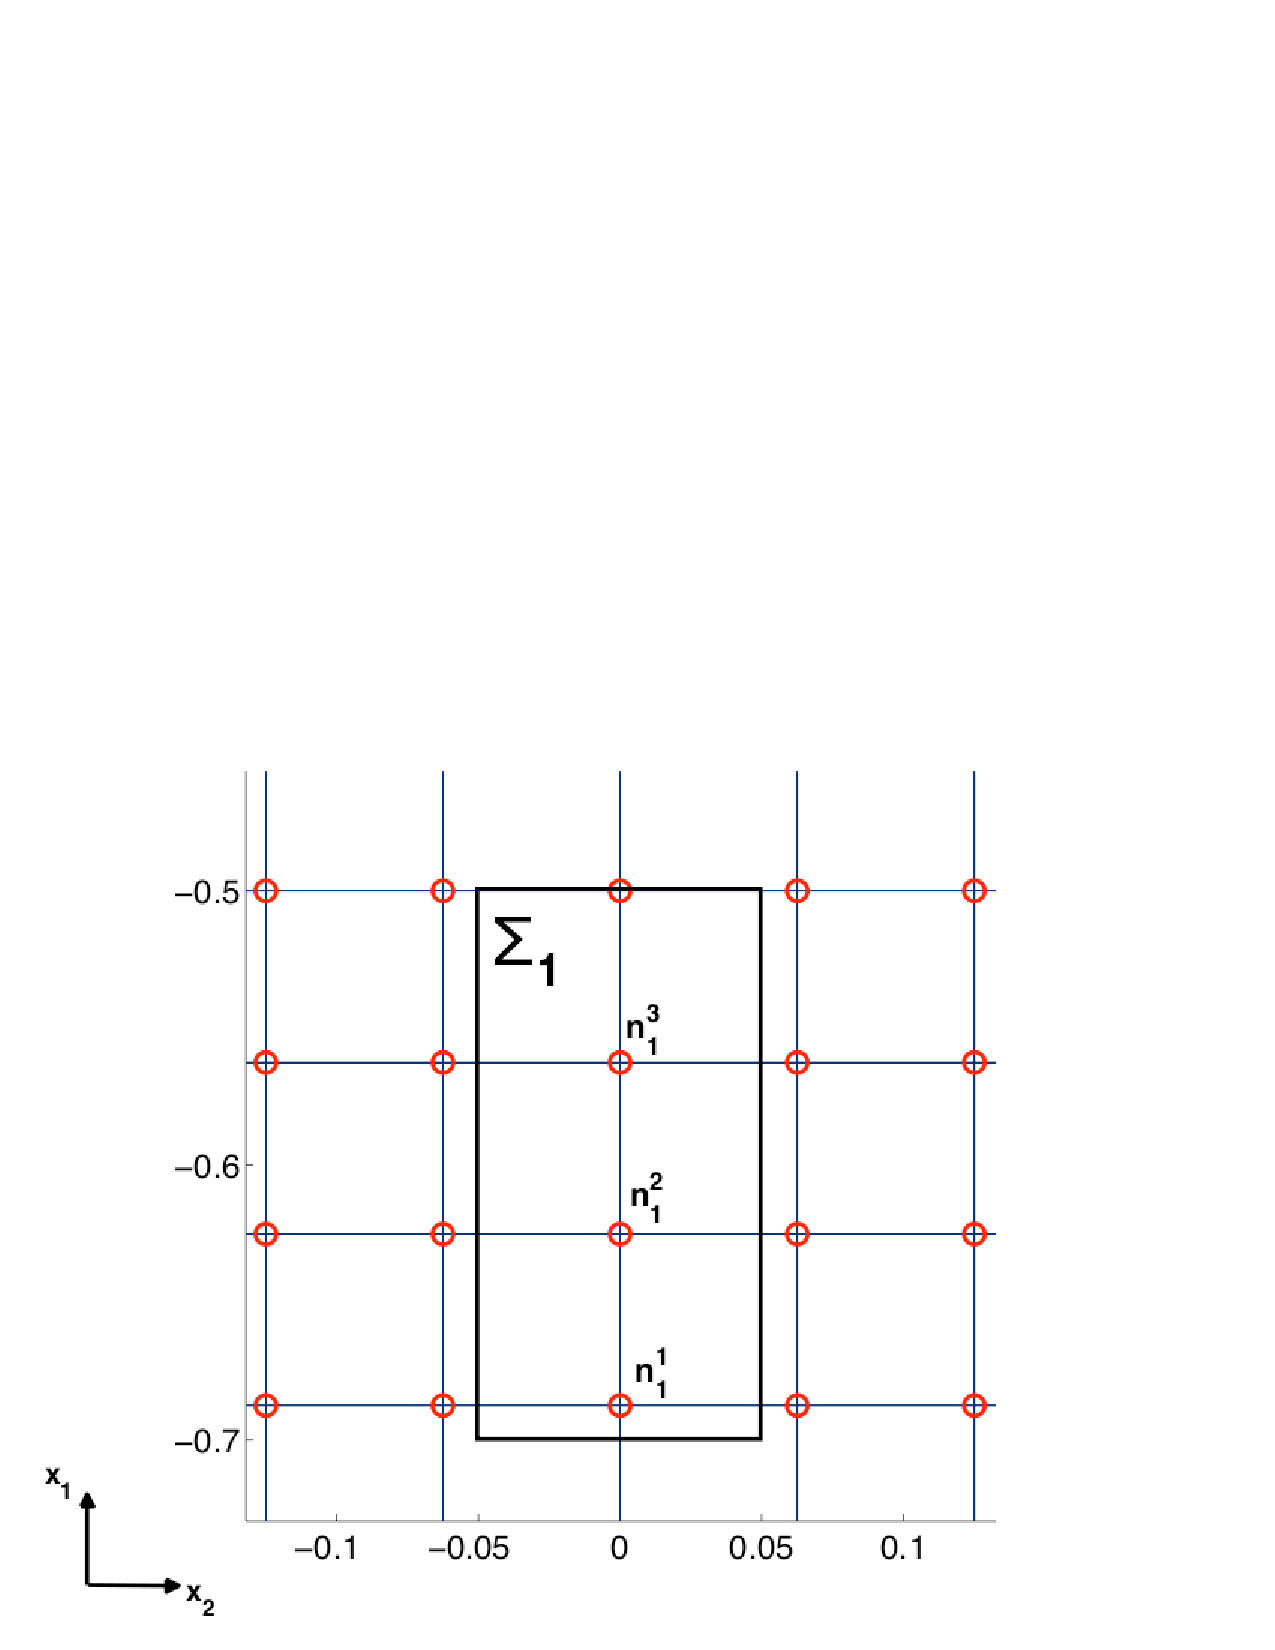
\includegraphics[width=5.6cm]{pics/numex/sigma1s.pdf}  
  %\end{minipage}
  \begin{minipage}[b]{6 cm}
    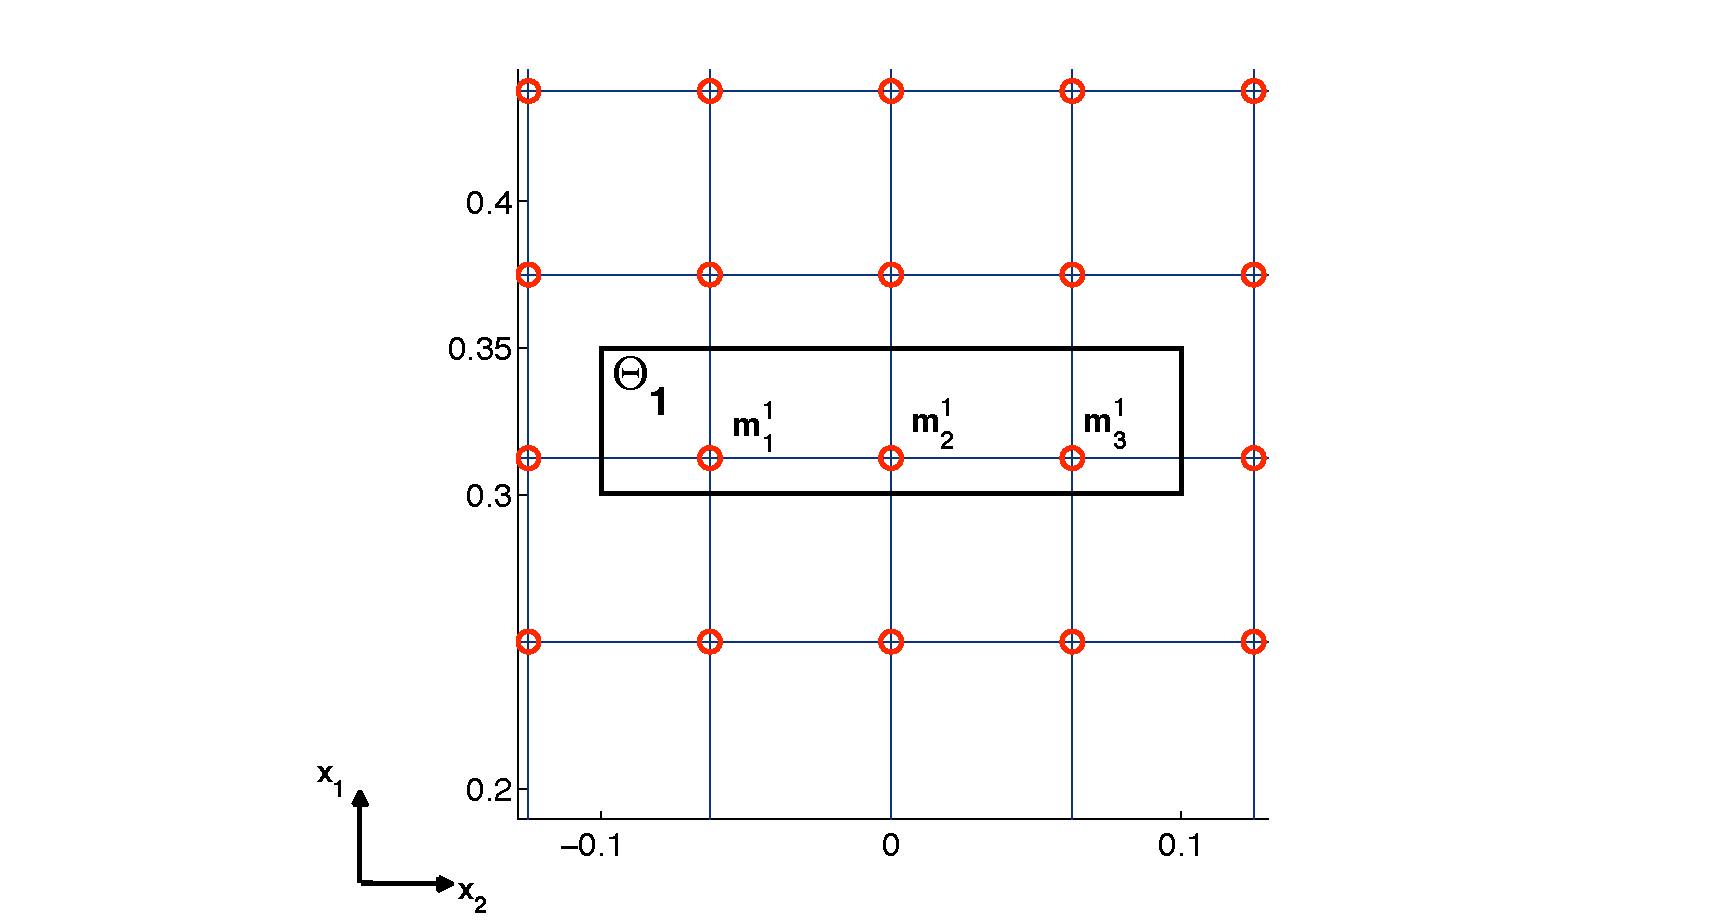
\includegraphics[width=6cm]{pics/numex/theta1s.pdf}
  \end{minipage}
  \caption{Distribution and enumeration of the velocity nodes in the reduced and observation domain}
  \label{sigthe1}
\end{figure}

Having established $U_h$ as in the previous section, one defines for $t \in [0,0.1]$ the input signal $\mathbf u_h(t) \in U_h$ via the coefficient functions $u_{x_1}^1,u_{x_2}^1 \in L^2(0,0.1)$:
\begin{equation*}
 \mathbf u_{1,h}(t) = u_{x_1}^1(t)\begin{bmatrix} \xi_1 \\ 0 \end{bmatrix}+u_{x_2}^1(t)\begin{bmatrix}0 \\ \xi_1 \end{bmatrix}
\end{equation*}
Here, e.g. $u_{x_1}(t)^1 \xi_1$ models the input signal of intensity $u_{x_1}(t)$ that acts in $x_1$-direction, uniformly distributed in the velocity nodes belonging to $\Sigma_1$.

The output was extracted via $C_{1,v}^T$ by computing $\bar{ \mathbf v}_h(t)$ which represents the average velocity over the nodes $ \mathfrak m_1^1,\mathfrak m_2^1,\mathfrak m_3^1$ pictured in Figure \ref{sigthe1}, giving the output signal
\begin{align*}
  \mathbf y_{1,h}(t) := \bar v_{x_1}(t)\begin{bmatrix} \zeta_1 \\ 0 \end{bmatrix} + \bar v_{x_2}(t)\begin{bmatrix}0\\ \zeta_1 \end{bmatrix}\\
\intertext{with}
\begin{bmatrix}\bar v_{x_1}(t) \\ \bar v_{x_2}(t) \end{bmatrix} := \frac{1}{3} \bigl [ \mathbf v_h(t, \mathfrak m_1^1)+\mathbf v_h(t, \mathfrak m_2^1)+\mathbf v_h(t, \mathfrak m_3^1) \bigr ]
\end{align*}
and $\zeta_1$ defined as in the previous section.

The temporal discretization was carried out by approximating the signal components in $L^2(0,0.1)$ by piecewise constant functions. Thereto the finite dimensional interpolation spaces $\mathcal R(k_1)$ and $\mathcal S(k_2)$ were defined by means of the \textit{Haar-wavelet} basis, i.e.
\begin{equation}\label{rswav}
 \mathcal R(k_1) = \spann \bigl \{ \varphi_i \bigr \} _{i=1}^{2^{k_1}} \andi 
 \mathcal S(k_2) = \spann \bigl \{ \varphi_j \bigr \} _{j=1}^{2^{k_2}}, \quad k_1,k_2 \in \mathbb N
\end{equation}
where $\varphi_l$ denotes the $l$-th \textit{Haar-wavelet} basis function in $[0,0.1]$, illustrated in Figure \ref{haars}.

This special choice equips the bases of $\mathcal R(k_1)$ and $\mathcal S(k_2)$ with the useful properties of orthogonal and hierarchical bases. The second means, that the signal discretization can be refined or coarsened by simply adding or removing basis functions, to change e.g. the degrees of freedom in $\mathcal R(k_1)$ from $2^{k_1}$ to $2^{k_1+1}$. 

The restriction of the levels of approximation to $\dim \mathcal R \in \{2^k,k\in \mathbb N\}$ ensures a uniform resolution on the whole time scale.

The projection of e.g. $u_{x_1}^1(t)$ and $\bar v_{x_1}(t)$ onto $\mathcal R(k_1)$ and $\mathcal S(k_2)$, respectively, is then realized by the \textit{discrete wavelet transform}, as described e.g. in \cite{wtsp}. To circumvent a possible aliasing error, c.f  \cite[Ch.~1]{cowa}, it was ensured that the time resolution of the input and output signals was sufficiently high. 

\begin{figure}[htbp]
  \centering
  \begin{minipage}[b]{4.8 cm}
    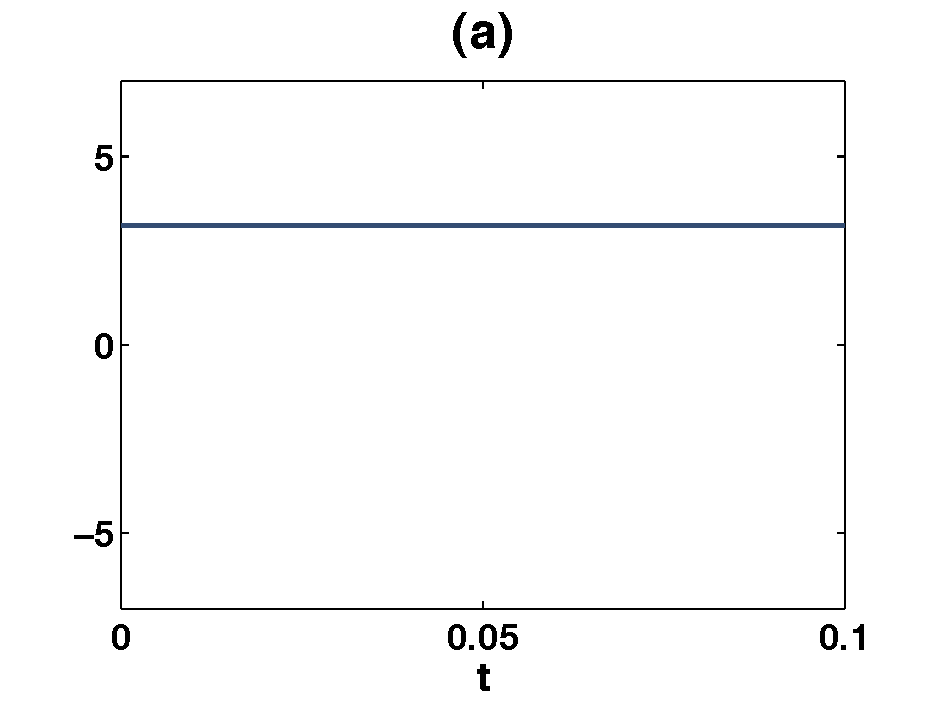
\includegraphics[width=4.8cm]{pics/wav1.pdf}  
  \end{minipage}
  \begin{minipage}[b]{4.8 cm}
    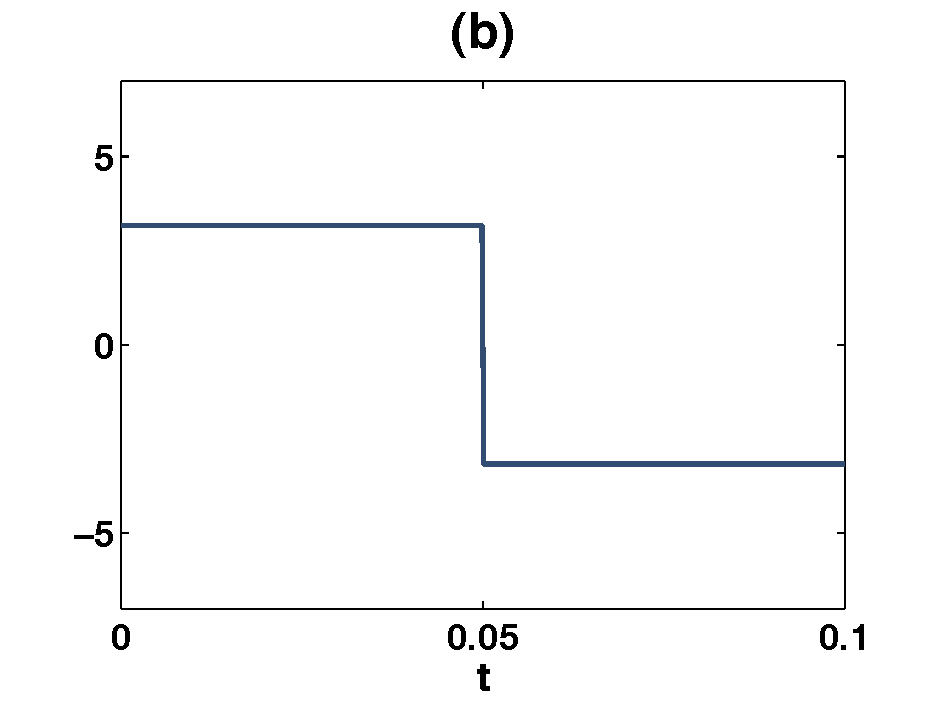
\includegraphics[width=4.8cm]{pics/wav2.pdf}  
  \end{minipage}
  \begin{minipage}[b]{4.8 cm}
    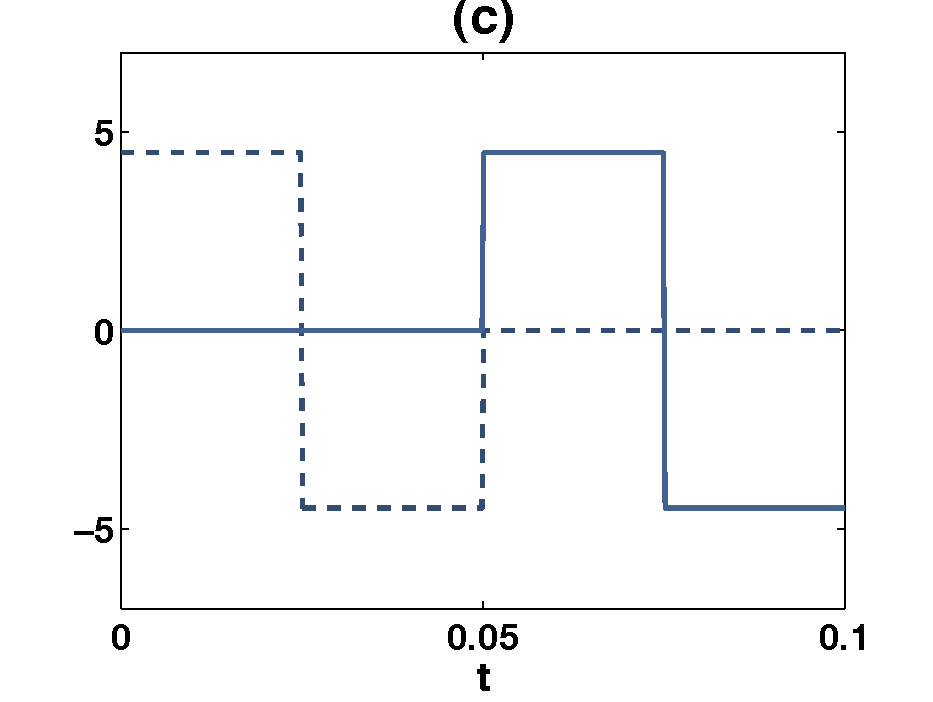
\includegraphics[width=4.8cm]{pics/wav34.pdf}  
  \end{minipage}
  \begin{minipage}[b]{4.8 cm}
    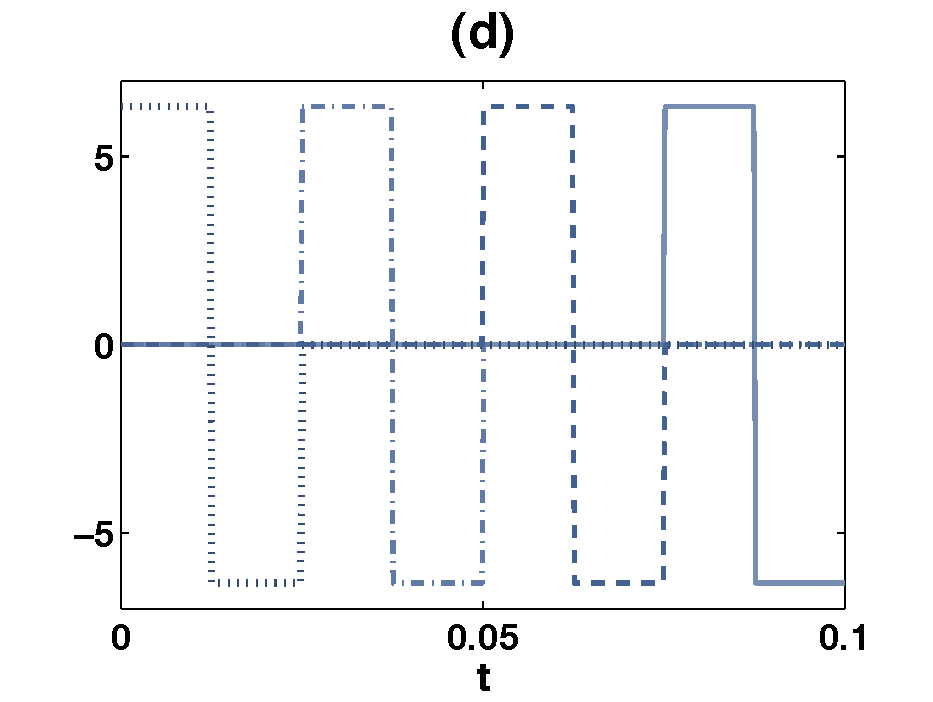
\includegraphics[width=4.8cm]{pics/wav5678.pdf}  
  \end{minipage}
  \caption{Orthonormal Haar wavelet basis of the $L^2(0,0.1)$ subspace of piecewise constant functions: (a) $\varphi_1$, (b) $\varphi_2$, (c) $\varphi_3,\varphi_4$, (d) $\varphi_5,\varphi_6,\varphi_7,\varphi_8$ }
  \label{haars}
\end{figure}

In view of the investigation of the approximation errors within the reduced test case,
\begin{equation*}
 \Gamma _{1,h}:\mathbf u_{1,h} \mapsto \mathbf y_{1,h}
\end{equation*}
was defined as the concrete realization of the input/output map defined in \eqref{osio} of the controlled driven cavity system:
\begin{align}\label{testcase1}
	\begin{bmatrix} M& 0 \\ 0& 0 \end{bmatrix} \frac{d}{dt} {\begin{bmatrix} \mathbf v_h(t) \\ \mathbf p_h(t)  \end{bmatrix}} + \begin{bmatrix} D& -B^T \\  B& \frac{1}{4}Q^* \end{bmatrix} \begin{bmatrix} \mathbf v_h(t) \\ \mathbf p_h(t)  \end{bmatrix} &= \begin{bmatrix} \mathbf f_h + \bar {\mathbf u}_{1,h}(t) \\ \mathbf g_h \end{bmatrix} \\
\mathbf y_{1,h}(t) &= C_{1,v}^T \mathbf v_h(t)\quad \quad \quad \text{ in $(0,0.1]$} \notag\\
\text{and  }\quad \quad \mathbf v(0) = \mathbf v_0& \notag
\end{align}
Here $\bar {\mathbf u}_{1,h}(t)$ represents $\mathbf u_{1,h}(t)$ in $Q_1(\Omega_h)$ and $ \mathbf v_0$ is the steady-state solution of the uncontrolled problem.

The extension to the full scale problem is straight forward. The domains of control and observation $\Sigma$ and $\Theta$ contain $3 \times 16$ and $9 \times 3$ velocity nodes, respectively. Defining the spaces $U_h$ and $Y_h$ as in the above Section \ref{dcdc} and the discrete signal coefficient spaces as for the test case one obtains

 \begin{subequations}
 \begin{align*}
  U_{h_1} = \spann \bigl\{ \mu_1,\dots,\mu_{32} \bigr\}, &\quad R_{k_1} = \spann \bigl \{ \varphi_i \bigr \}^{2^{k_1}}_{i=1}\\
\text{and} \quad
 Y_{h_2} = \spann\bigl \{ \nu_1,\dots,\nu_{18} \bigr\}, & \quad S_{k_2} = \spann\bigl \{ \varphi_j \bigr \}^{2^{k_2}}_{j=1}
 \end{align*}
\end{subequations}
to define the input signals and to display the output.


\subsection{Convergence in the Signal Approximation}

For the convergence tests, the reduced testcase introduced in the previous section was considered. To compute $\mathbf y_{1,h}(t) :=\Gamma _{1,h}\mathbf u_{1,h}(t)$ for $t\in(0,0.1]$ system \eqref{testcase1} was integrated using \textit{Projection2} with a step size of $2.5 \cdot 10^{-4}$.

Let $\mathscr P_k$ denote the \textit{discrete wavelet transform} for a signal using the first $2^k$ \textit{Haar-wavelets}. The projector $\mathscr P_k$ is used to project the signal coefficients onto the finite dimensional subspaces $\mathcal R(k_1)$ and $\mathcal S(k_2)$ as defined in \eqref{rswav}.

In line with the notation for the theoretical error analysis in Section \ref{sae} the input and output interpolation errors are defined as $e_{u_1,hk_1}:=\mathbf u_{1,h}-\mathscr P_{k_1}\mathbf u_{1,h}$ and $e_{y_1,hk_2}= \mathbf y_{1,h}-\mathscr P_{k_2}\mathbf y_{1,h}$, respectively.

Proposition \ref{aper} states that the signal approximation error can be estimated via the sum of $e_{y_1,hk_2}$ and the system response of the input interpolation error $\Gamma _{1,h}e_{u_1,hk_1}$, measured in the $\mathcal Y = L^2[0,0.1;Q_1(\Omega_h)]$ norm:
\begin{equation*}
 \norm{\Gamma _{1,h}\mathbf u_{1,h} - \mathscr P_{k_2}\Gamma _{1,h}\mathscr P_{k_1}\mathbf u_{1,h}}_{\mathcal Y} \leq \norm{e_{y_1,hk_2}}_{\mathcal Y} + \norm{\Gamma _{1,h}e_{u_1,hk_1}}_{\mathcal Y}
\end{equation*}


The wavelet interpolation of level $k_1$ and $k_2$ uses piecewise constant functions on subintervals of size $0.1/2^{k_1} =: \kappa_1$ and $0.1/2^{k_2} =: \kappa_2$, respectively, and the wavelet transform produces an error, that decreases linear with a refinement of the discretization. 

Thus, in the present case one has $\norm{e_{y_1,hk_2}}_{\mathcal Y}=\mathcal O(\kappa_2)$. Also, using again Proposition \ref{aper}, one has $\norm{\Gamma _{1,h}e_{u_1,hk_1}}_{\mathcal Y}=C\norm{e_{u_1,hk_1}}_{\mathcal U}=\mathcal O(\kappa_1)$ with system specific constant $C$.

For the convergence test, the input signal was set to
\begin{equation*}
 \mathbf u^s_{1,h}(t) = s(t)\begin{bmatrix} \xi_1 \\ 0 \end{bmatrix}
\end{equation*}
with a test signal $s \in \mathcal C(0,0.1)$ as shown in Figure \ref{sigap} (a). The response is denoted by $\mathbf y^s_{1,h}(t) :=\Gamma _{1,h}\mathbf u^s_{1,h}(t)$ and illustrated by its $x_1$-component in Figure \ref{sigap} (b).

\begin{figure}[htbp]
  \centering
  \begin{minipage}[b]{6 cm}
    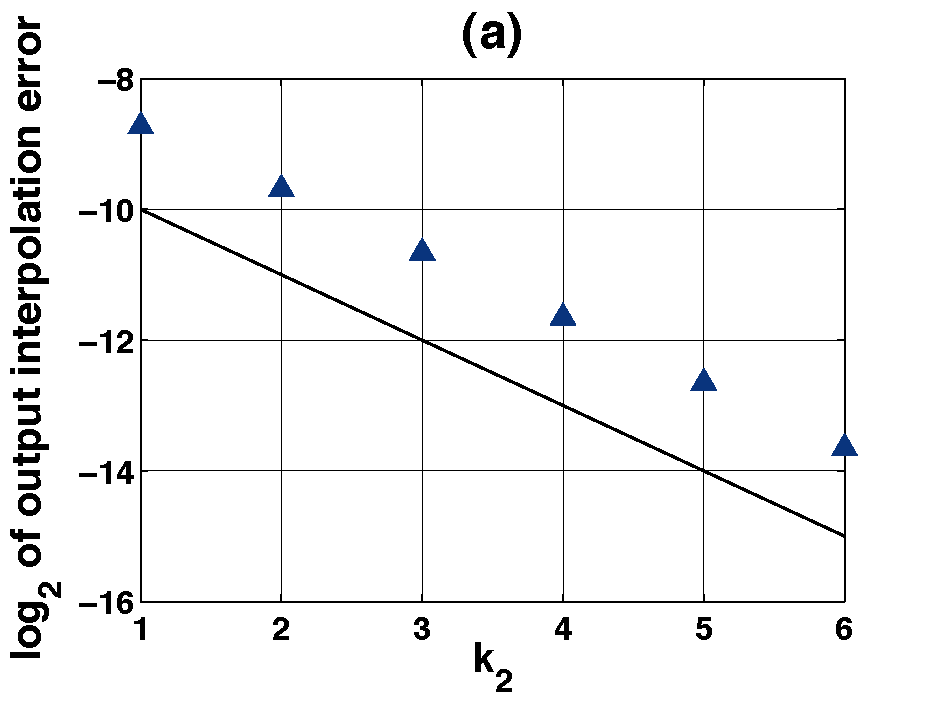
\includegraphics[width=6cm]{pics/numex/outintplot.pdf}  
  \end{minipage}
  \begin{minipage}[b]{6 cm}
    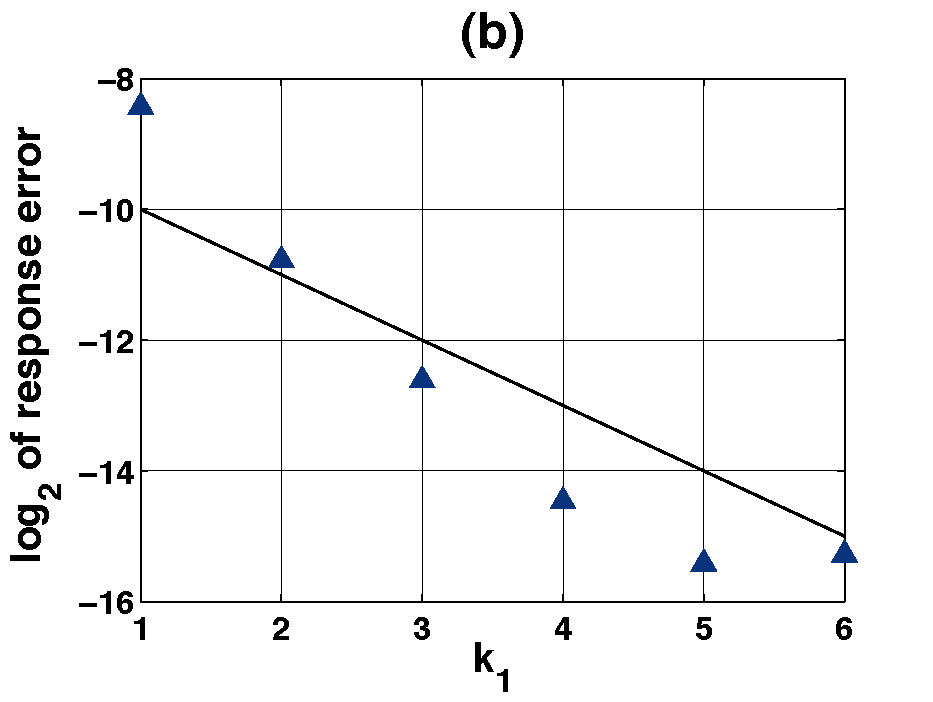
\includegraphics[width=6cm]{pics/numex/resperplot.pdf}  
  \end{minipage}
  \caption{(a) The $2~\log$ of the error $\norm{e_{y_1,hk_2}}_{\mathcal Y}$ of the signal approximation in the output space using the first $2^{k_2},~k_2=1,..,6$ \textit{Haar-wavelet} basis functions for the approximation. Part (b) shows the error in the response $\norm {\Gamma _he_{u_1,hk_1}}_{\mathcal Y}$ in the output space, caused by the approximation of the input signal $\mathbf u^s_{1,h}$ by means of $2^{k_1},~k_1=1,..,6$ \textit{Haar-wavelet} basis functions. The straight line denotes the slope of a linear convergence}
  \label{sigapcon}
\end{figure}

As displayed in Figure \ref{sigapcon} the interpolation $\norm{e_{y_1,hk_1}}_{\mathcal Y}$ error shows the expected linear behaviour. The quadratic convergence of $\norm {\Gamma _he_{u_1,hk_1}}_{\mathcal Y}$ for smaller resolutions points to a smoothing property of the considered system. This property is also evident in the illustration in Figure \ref{sigap} and in the dissymmetry in the matrix of the relative errors shown in table \ref{errma}. For $k_{1},k_{2} \geq 2$ the values above the diagonal are significant smaller than their counterpart the transposed value. This implies that in the given test case it is worthier to do an refinement in the response space rather than in the input space. 


\begin{figure}[htbp]
  \centering
  \begin{minipage}[b]{6 cm}
    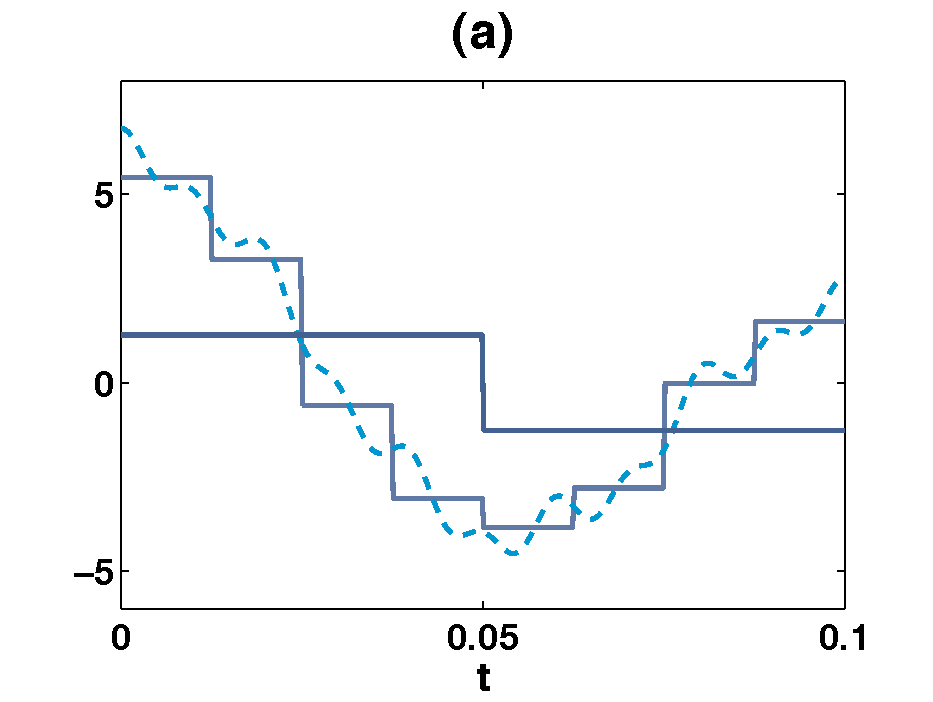
\includegraphics[width=6cm]{pics/fullOpti/new/testSig_ul1_ul3.pdf}  
  \end{minipage}
  \begin{minipage}[b]{6 cm}
    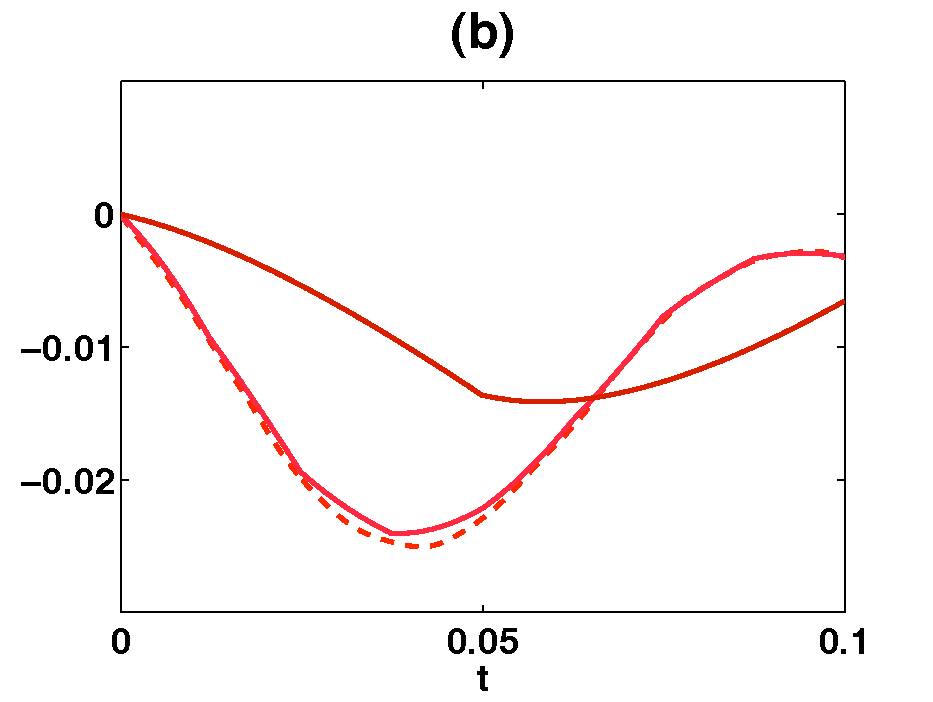
\includegraphics[width=6cm]{pics/fullOpti/new/testSig_yl1_yl3.pdf}  
  \end{minipage}
  \caption{Illustration of (a) the approximation of the test signal $s$, denoted by the dotted line, in the input space using the first 2 and 8 Haar wavelet basis functions and (b) of the $x_1$-component of the respective response in the output space }
  \label{sigap}
\end{figure}

\begin{table}[htbp]
\centering
\begin{tabular}{c|cccccc}
 $k_{1} \backslash k_{2}$ & $1$ & $ 2$ & $3$ & $4$ & $5$ & $6$ \\ 
\hline
 $1$ & $    \textbf{1.0000 }$ & $    0.8744 $ & $    0.8561 $ & $    0.8520 $ & $    0.8510  $ & $   0.8508$ \\
  $2$&$   0.7061 $&$   \textbf{0.3896} $&$   0.2440  $&$  0.1899  $&$  0.1738  $&$  0.1696$ \\
  $3$&$  0.6922  $&$  0.3585  $&$  \textbf{0.1870}  $&$  0.1022  $&$  0.0658  $&$  0.0529$ \\
 $4$&$   0.6911 $&$   0.3559  $&$  0.1817  $&$  \textbf{0.0919}  $&$  0.0475 $&$   0.0266$ \\
 $5  $&$0.6910  $&$  0.3558 $&$   0.1814 $&$   0.0912  $&$  \textbf{0.0460}  $&$  0.0237$ \\
  $6 $&$  0.6911 $&$   0.3558  $&$  0.1814 $&$   0.0912 $&$   0.0460  $&$  \textbf{0.0237}$ \\

\end{tabular}
\caption{Matrix of the relative error $\norm{\Gamma _{1,h}\mathbf u^s_{1,h} - \mathscr P_{k_2}\Gamma _{1,h}\mathscr P_{k_1}\mathbf u^s_{1,h}}_{\mathcal Y}/e_{11}$ caused by approximating the input signal and corresponding response signal by means of Haar wavelets using $2^{k_1}$ and $2^{k_2}$ basis functions. In the lines $k_1$ denotes the level of the of the approximation of the input signal, in columns $k_2$ stands for the degree of the interpolation of the response. The normalization $e_{11}$ is the error for $k_1=k_2=1$}
\label{errma}
\end{table}

\section{Optimal Control}
The goal of an optimal control of the system described above is to find a control $\mathbf u_h^* \in \mathcal U_h = L^2(0,0.1;U_h)$ that delivers the desired output $\mathbf y_h^* \in \mathcal Y_h = L^2(0,0.1;Y_h)$. Given a corresponding input/output map $\Gamma_h$ the unconstrained optimization problem is defined by
\begin{prob}\label{optprob}
Given $\mathbf y_h^* \in \mathcal Y_h$ find $\mathbf u_h \in \mathcal U_h $ such that 
 \begin{equation*}
 \norm{\mathbf y_h^* - \Gamma_h \mathbf u_h}^2_{\mathcal Y_h} \rightarrow \min
\end{equation*}
\end{prob}





\subsection{I/O Map for the Driven Cavity}
In line with the mathematical framework of Section \ref{diom} the matrix representation of the input/output map is established by computing the system response basis functions of the input space $\mathcal U_{hk_1}$ and testing them against all basis functions of the output space $\mathcal Y_{hk_2}$. In the present case, one has for the input and output space
\begin{subequations}\label{uhkyhk}
 \begin{align}
  \mathcal U_{hk_1} = \spann \bigl \{ \mu_l\varphi_j: l=1,\dotsc,32,~j=1,\dotsc,{2^{k_1}} \bigr \}
\intertext{and}
  \mathcal Y_{hk_2} = \spann \bigl \{ \nu_k\varphi_i: k=1,\dotsc,18,~i=1,\dotsc,{2^{k_2}} \bigr \}
 \end{align}
\end{subequations}
respectively. Thus the block-structured matrix 
\begin{align*}
 \mathbf H &= \left[H ^ {kl}  \right] _{\substack{k=1,\dotsc,18\\ l = 1,\dotsc,32} }, \quad \text{with} \\
  & H ^ {kl} = \left [ (\nu_k \varphi_i,G_h(\mu_l\varphi_j))_{\mathcal Y} \right]_{\substack{i=1,\dots,2^{k_2} \\ j = 1,\dots,2^{k_1}}} 
\end{align*}
maps the input signal coefficient vector $\mathbf u_{hk_1} \in \mathbb R ^ {32 \cdot 2^{k_1}}$ onto $M_{\mathcal Y} \mathbf y_{hk_2}$, where $M_{\mathcal Y}$ denotes the mass matrix corresponding to the discretization of $\mathcal Y_{hk_2}$ and $\mathbf y_{hk_2} \in \mathbb R ^{18\cdot 2^{k_2}}$ the coefficient vector of the discretized system response.


\begin{rem}
The signal response $\mathbf y_h = G_h(\mathbf u_h)$ is computed by numerical integration of the semidiscretized state equations, i.e. $\mathbf y$ is a vector containing the function values at discrete points within the time interval. The time integral of the inner product $(\mathbf y_h , G_h(\mathbf u_h))_{\mathcal Y}$ and the norm $\norm{\mathbf y_h}_{\mathcal Y}$ are then approximated using piecewise the trapezoidal rule, which causes an inaccuracy of order $2$ with respect to the time step used in the \textit{Projection2} algorithm. Recalling that the \textit{Projection2} algorithm produces a time integration error of first order, this error is neglected. 
\end{rem}

\subsection{Realization}
In the following formulations, especially when speaking of concrete realizations, the subscripts of the coefficient vectors $\mathbf y_{hk_1}$ and $\mathbf y_{hk_2}$ are dropped.

Using the discretized signal spaces $\mathcal U_{hk_1}$ and $\mathcal Y_{hk_2}$ the optimization problem can be solved approximately by finding an optimal input coefficient vector $\mathbf u$ and considering its response $M_{\mathcal Y} \mathbf y = \mathbf H \mathbf u$. The definition of $G_h$ \eqref{ioms} required the subtraction of the constant offset $\mathbf y_{0,h}$, which has to be added to the output to obtain the actual state. Thus the approximated Problem \ref{optprob} reads
\begin{prob}\label{apoppr}
Given $\mathbf y_h^* \in \mathcal Y_h$ find $\mathbf u \in \mathbb R  ^ {32 \cdot 2^{k_1}}$ such that 
 \begin{equation}\label{objfun1}
 \norm{\mathbf y_h^* - (\mathbf y_{0,h} + \kappa_{\mathcal Y_h}^{-1} M_{\mathcal Y}^{-1} \mathbf H \mathbf u )}^2_{\mathcal Y} \rightarrow \min
\end{equation}
\end{prob}
where $ \kappa_{\mathcal Y}^{-1}$ maps the coefficient vector $M_{\mathcal Y}^{-1}{\mathbf y}$ onto the corresponding function in $\mathcal Y_{hk_2}$. 

\subsection{Application Examples}

For a start, a one dimensional in space example is presented to illustrate the principle of the optimization.

Thereto the reduced testcase introduced in Section \ref{redteca} was considered, which models the input signal by means of two spatial basis functions and $2^{k_1}$ temporal basis functions. Also, the output possesses two degrees of freedom in space, representing the components of the mean velocity around the sensor point, and $2^{k_2}$ degrees of freedom in the time discretization. 

The goal of the optimization was to find a control $\mathbf u^*_{1,h} \in \mathcal U_h$ such that the $x_1$-component of the response $\Gamma _{1,h}\mathbf u^*_{1,h} \in \mathcal Y_h$ is zero. 

Thereto the corresponding optimization Problem \ref{apoppr} was considered to compute an approximate solution on the basis of the discretized signal spaces $\mathcal U_{hk_1}$ and $\mathcal Y_{hk_2}$.

Find $\mathbf u^*_{1}\in \mathbb R^{2\cdot k_1}$ such that
\begin{equation*}
 \norm{\bigl [y_{0,h} + \kappa_{\mathcal Y}^{-1} M_{\mathcal Y}^{-1} \mathbf H_1 \mathbf u^*_{1}\bigr ]_{x_1} }^2_{\mathcal Y_h} \rightarrow \min,
\end{equation*}
using the i/o map $\mathbf H_1 \in \mathbb R ^{1 \cdot 2^{k_2} \times 2 \cdot 2^{k_1}}$.

The optimization was run for $k_1,k_2 \in \{4,5,6\}$ to find an appropriate optimal solution $\mathbf u^*_{1}(k_1,k_2)$, using the line search algorithm of the Matlab \cite{matl} function \texttt{fminunc}. As the start value $\mathbf u = 0$ was chosen. The result for $k_1=k_2=5$ is displayed in Figure \ref{1dopti}.

\begin{figure}[htbp]
  \centering
  \begin{minipage}[b]{6 cm}
    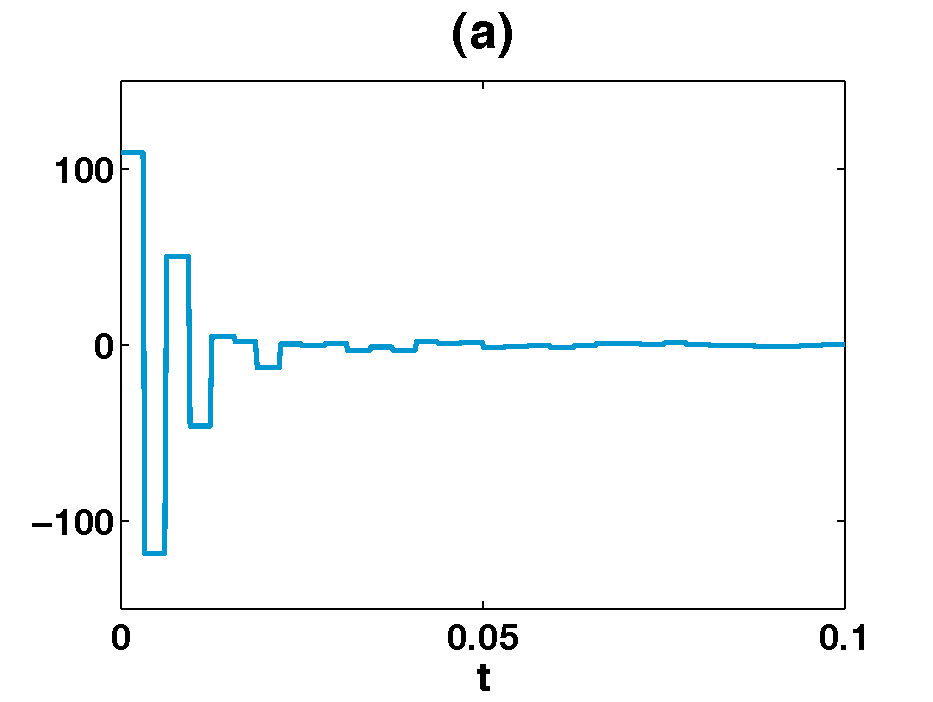
\includegraphics[width=6cm]{pics/1doptiinp.pdf}  
  \end{minipage}
  \begin{minipage}[b]{6 cm}
    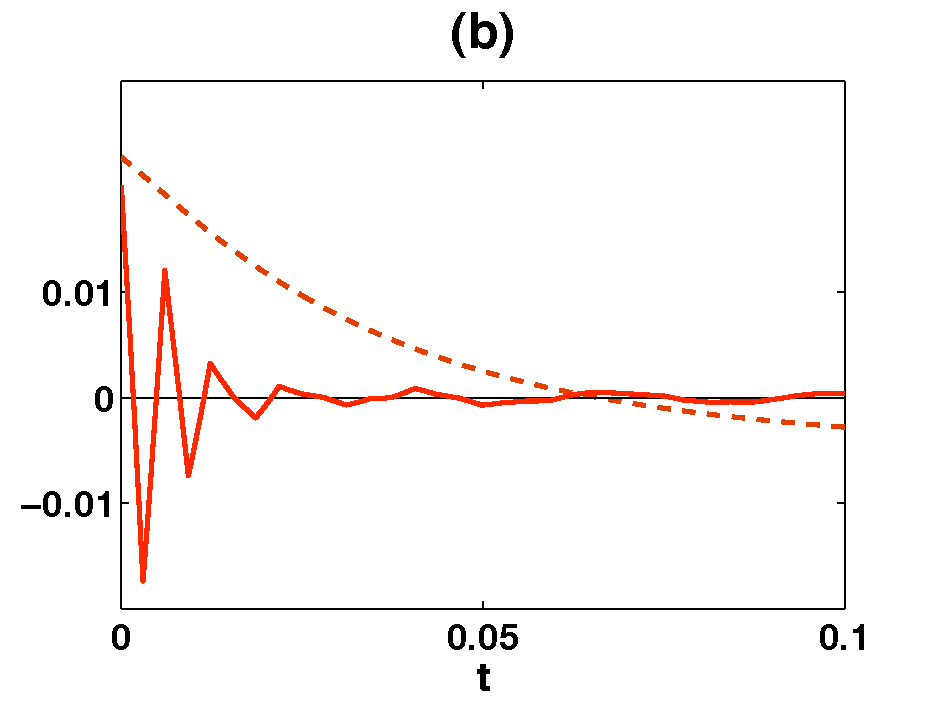
\includegraphics[width=6cm]{pics/1doptires.pdf}  
  \end{minipage}
  \caption{The $x_1$-component of the optimized signal $\mathbf u_{1}(k_1,k_2) ^*$ for $k_1= k_2 = 5$ (a), intented to force a zero $x_1$-component in the output (b) . The dotted line in (b) shows the ''uncontrolled`` solution } 
\label{1dopti}
\end{figure}

The continuous in time system response $\Gamma_{1,h} \mathbf u^*_{1}(k_1,k_2)$ for all combinations of $k_1,k_2$ were computed to check the optimality properties of the computed inputs. 

The norm of the $x_1$-component of  $r_{k_1,k_2} := \norm{\bigl [\Gamma_{1,h} \mathbf u^*_{1}(k_1,k_2)\bigr ]_{x_1}}_{\mathcal Y}^2$ describes the distance of the computed discrete solution to a possible optimal continuous solution. Table \ref{rema} shows the residuals for $k_1,k_2 = 4,5,6$. 

\begin{table}[htbp]
\centering
\begin{tabular}{c|ccc}
$k_1 \backslash k_2$ & $4$ & $5$ & $6$ \\ 
\hline
$4  $& $1$ &$0.8 $&$ - $\\ 
$5  $&$0.365$ &$0.45  $&$  0.388 $\\
$6 $& $0.277$&$  0.154$&$   0.17  $ \\

\end{tabular}
\caption{Matrix of the relative residuals $r_{k_1,k_2}$ normalized by scaling with $r_{4,4}$.}
\label{rema}
\end{table}

It is notable that the values below the diagonal are much smaller than their counterparts above the diagonal. This is probably due to a better performance of the optimization algorithm in an overdetermined rather than in an underdetermined system. For the extreme case $2^4$ inputs versus $2^6$ outputs the optimization algorithm found no satisfiable solution.

For the fullcase the complete discrete input and output spaces $\mathcal U_{hk_1}$ and $\mathcal Y_{hk_2}$ defined by \eqref{uhkyhk} are considered. On the basis of Table \ref{rema} it was decided to set $k_1=5$ and $k_2=4$ as the best compromise between low dimensionality and accuracy. Thus one obtains for the dimension of the input and output spaces  $\dim \mathcal U_{hk_1}=32\cdot 32$ and $\dim \mathcal Y_{hk_2} = 18 \cdot 16$. 

Accordingly for a given target state $\mathbf y_h^* \in \mathcal Y_h $, the approximate optimization Problem \ref{apoppr} is defined via: Find $\mathbf u^* \in \mathbb R ^{32 \cdot 32}$, such that
\begin{equation*}
 \norm{\mathbf y_h^* - (\mathbf y_{0,h} + \kappa_{\mathcal Y}^{-1} M_{\mathcal Y}^{-1} \mathbf H\mathbf u^* }^2_{\mathcal Y} \rightarrow \min
\end{equation*}
with the i/o map $\mathbf H \in \mathbb R ^{18 \cdot 16 \times 32 \cdot 3 2}$.

In the first realization the concrete target function $\mathbf y_h^*$ was chosen as $\mathbf y_h^{1*} = \bigl [[\mathbf y_h^{1*}]_{x_1}^T~[\mathbf y_h^{1*}]_{x_2}^T \bigr ]^T := \bigl [ \mathbf 1 ~ \mathbf 0 \bigr ]^T$ indepent of $t$. This choice models a state of an average $x_1$-velocity of $1$ and zero velocity in $x_2$-direction, uniformly distributed in the observation domain.

Again the \textsc{Matlab} function \texttt{fminunc} was taken to compute a satisfactory optimal solution vector $\mathbf u^{1*}$, starting with $\mathbf u = 0$. The optimality was checked by computing the continuous system response $\mathbf y^{1*} =\Gamma_h \mathbf u^{1*}$.

The result of this optimization is displayed by plotting $6$ of the $18$ components of $\mathbf y^{1*}(t)$ versus $t\in [0,0.1]$, see Figure \ref{x1res}.  A further illustration is given by  the velocity vector plot and the streamline plot at time $t=0.1$ for the driven cavity, controlled by the input $\mathbf u^{1*}$, see Figure \ref{x1vest}. According to the definition of the output, the chosen components of $\mathbf y^{1*}(t)$ represent the averaged in $x_2$-direction velocity components in the observation domain, measured at the sensor points indicated in Figure \ref{x1vest} (b). 


\begin{figure}[htbp]
  \centering
  \begin{minipage}[b]{6 cm}
    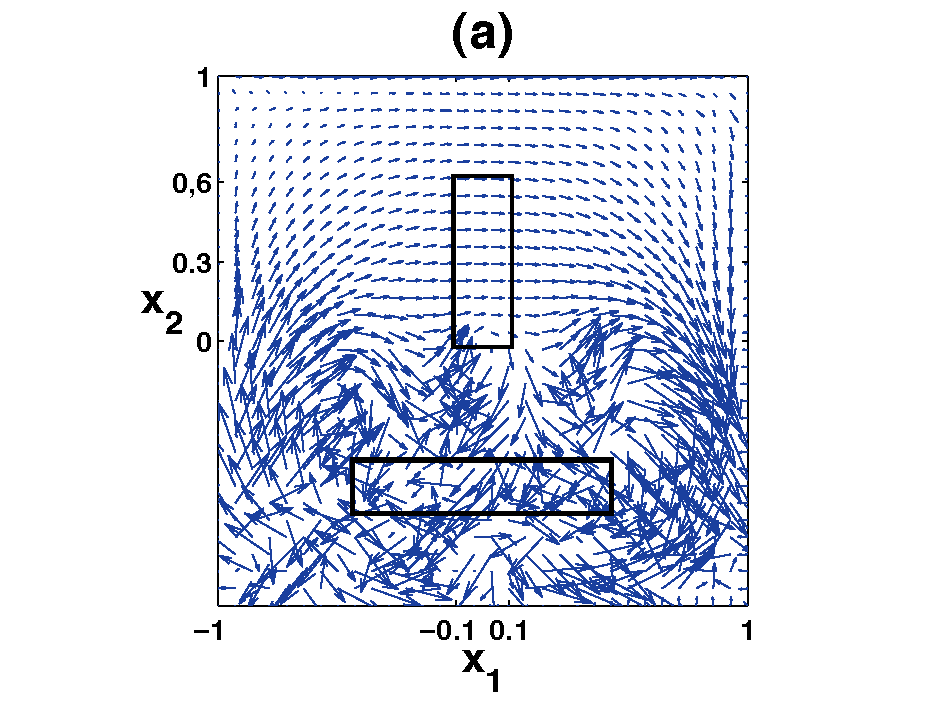
\includegraphics[width=6cm]{pics/fullOpti/new/x1_vear.pdf}
  \end{minipage}
  \begin{minipage}[b]{6 cm}
    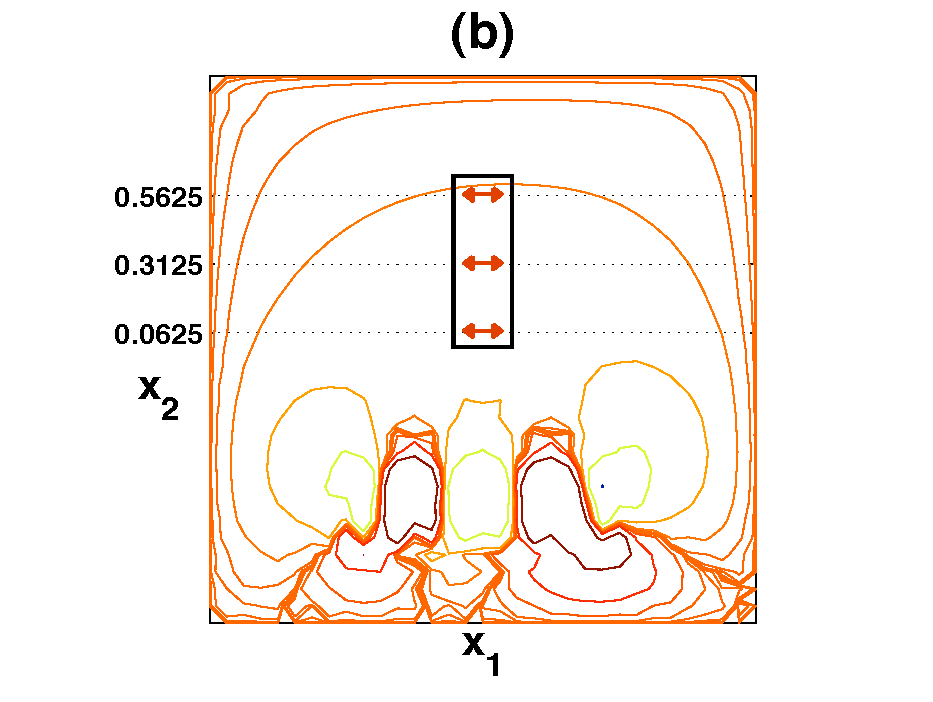
\includegraphics[width=6cm]{pics/fullOpti/new/x1_stli.pdf}
  \end{minipage}
   \caption{Velocity vector plot (a) and streamline plot (b) of the controlled Oseen driven cavity flow at time $t=0.1$, influenced by the input signal $u^{1*}$, optimized with respect to a uniform velocity distribution ($v_x = 1,~v_y=0$) within the time interval $[0,0.1]$ in the observation domain. The arrows in (a) indicate the positions of the extraction of the output signals belonging to $y^{1*}$, which are displayed in Figure \ref{x1res}.} 
\label{x1vest}
\end{figure}

\begin{figure}
\centering
 \begin{minipage}[b]{5cm}
    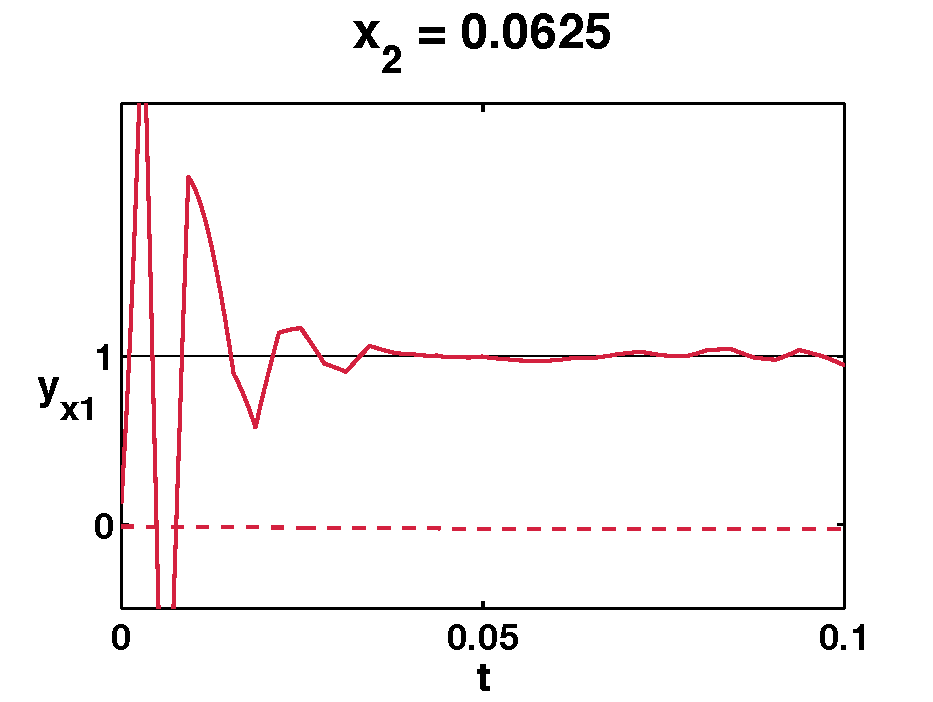
\includegraphics[width=5cm]{pics/fullOpti/new/x1_sigx2_1.pdf}  
  \end{minipage}
 \begin{minipage}[b]{5cm}
    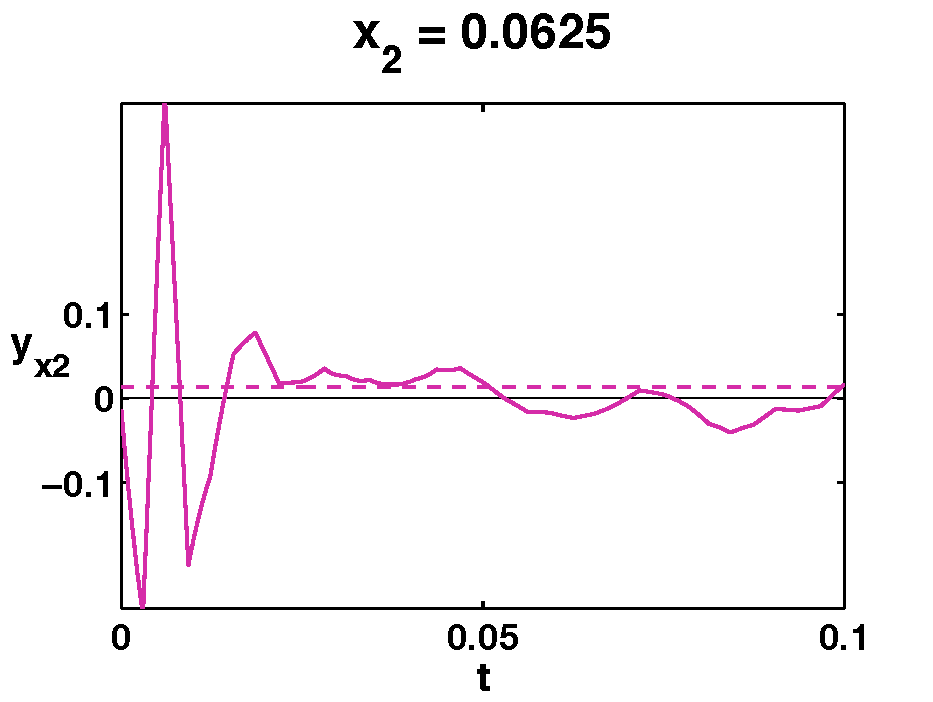
\includegraphics[width=5cm]{pics/fullOpti/new/x1_sigx22_1.pdf}  
  \end{minipage}
\vspace{0.3cm}
 \begin{minipage}[b]{5cm}
    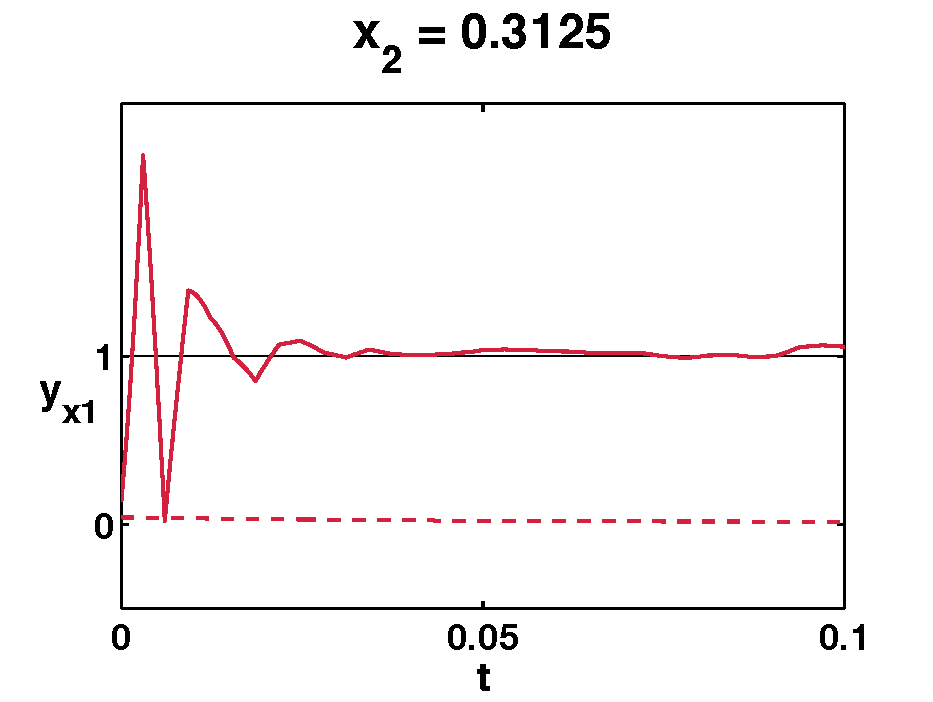
\includegraphics[width=5cm]{pics/fullOpti/new/x1_sigx2_2.pdf}  
  \end{minipage}
 \begin{minipage}[b]{5cm}
    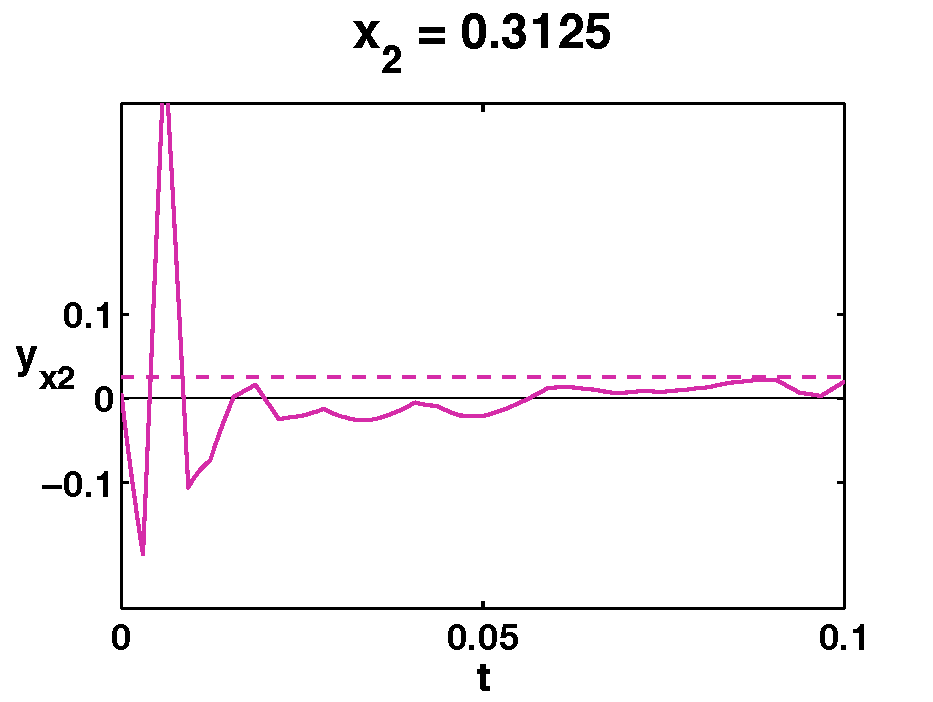
\includegraphics[width=5cm]{pics/fullOpti/new/x1_sigx22_2.pdf}  
  \end{minipage}
\vspace{0.3cm}
 \begin{minipage}[b]{5cm}
    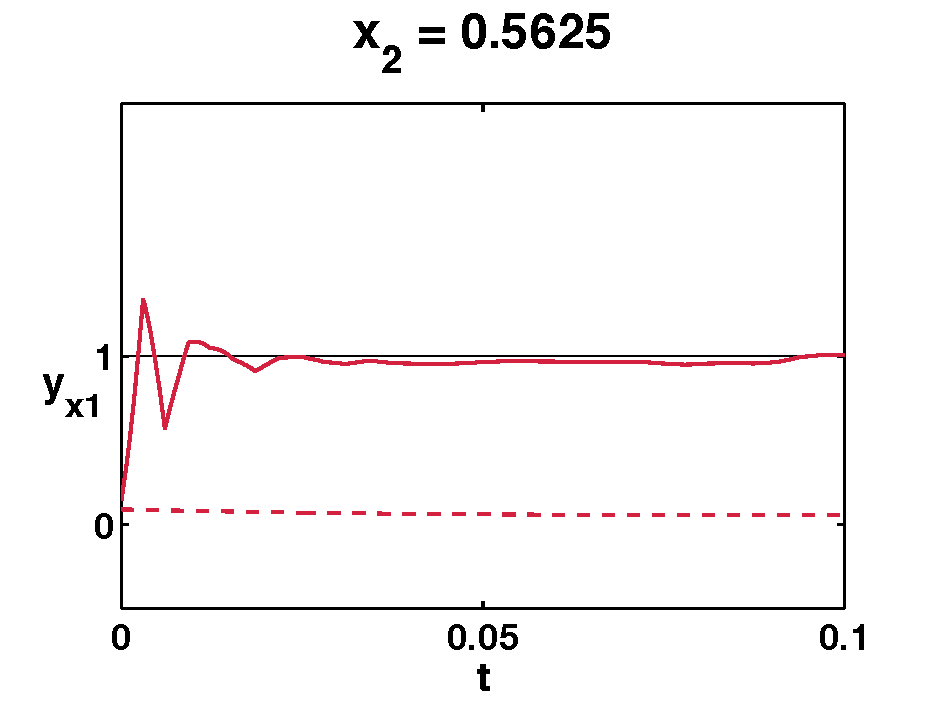
\includegraphics[width=5cm]{pics/fullOpti/new/x1_sigx2_3.pdf}  
  \end{minipage}
 \begin{minipage}[b]{5cm}
    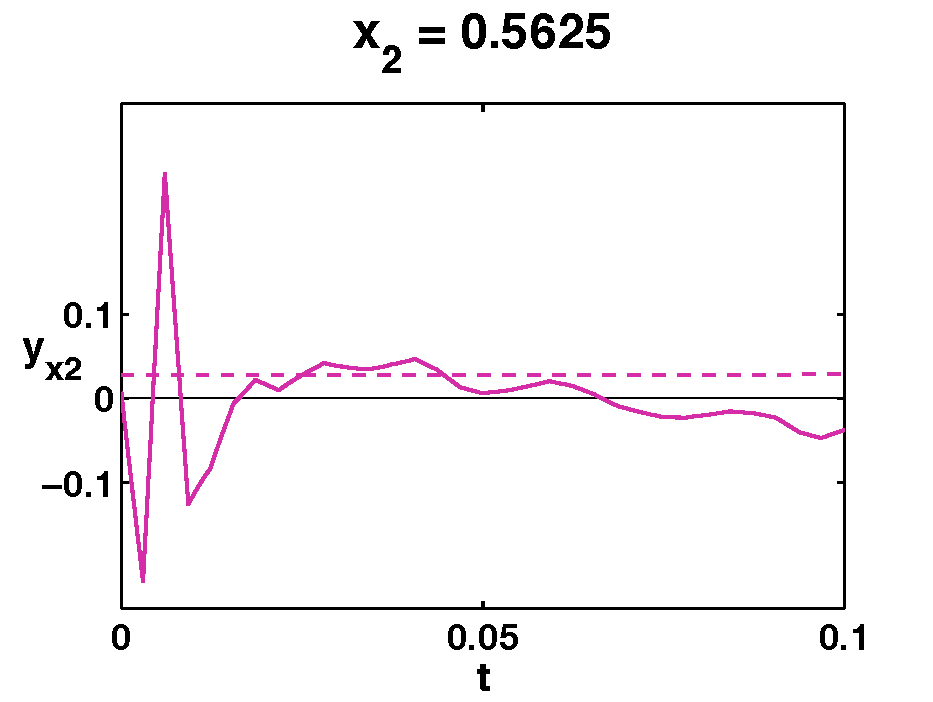
\includegraphics[width=5cm]{pics/fullOpti/new/x1_sigx22_3.pdf}  
  \end{minipage}
   \caption{6 components of the signal response $\mathbf y_h^{1*}$. The plots on the left-hand side show the $x_1$-component of the output at the sensor positions indicated in Figure \ref{x1vest} versus the time $t\in [0,0.1]$. The right-hand side displays the corresponding $x_2$-component. The dotted lines mark the corresponding ''uncontrolled`` outputs.} 
\label{x1res}
\end{figure}

Judging by the velocity vector plot in Figure \ref{x1vest} the target is obviously captured. Also the signal responses in Figure \ref{x1res} tend to the defined target state. Notably are the oscillations at the start, possibly induced by the initial gap between the target and the actual state. The ocurrence of these fluctuations in the $x_2$-component, where the gap to the target is much smaller, can be explained by the velocity coupling via the continuity equation. Having overcome these sharp oscillations the output stays within a certain proximity to the target. The still observable deviations are of the same order for both components, but better visible in the plots for the $x_2$-output due to the different scale for the vertical axis. 

Similar results are obtained with the same procedure but with the reversed target state $\mathbf y_h^{2*} := \bigl [[\mathbf y_h^{2*}]_{x_1}^T~[\mathbf y_h^{2*}]_{x_2}^T \bigr ]^T := \bigl [ \mathbf 1~ \mathbf 0 \bigr ]^T$. The plots for this second optimization, i.e. for the corresponding optimized signal $\mathbf u^{2*}$ and its response $\mathbf y^{2*}$, are displayed in Figure \ref{x2vest} and \ref{x2res}.

\begin{figure}[htbp]
  \centering
  \begin{minipage}[b]{6 cm}
    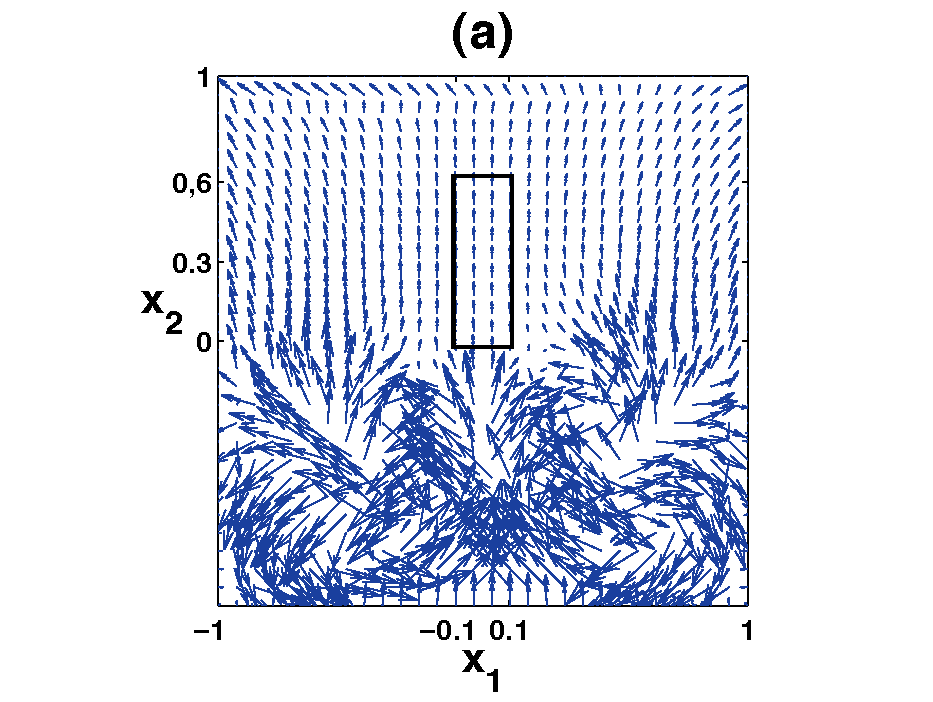
\includegraphics[width=6cm]{pics/fullOpti/new/vear_x2.pdf}
  \end{minipage}
  \begin{minipage}[b]{6 cm}
    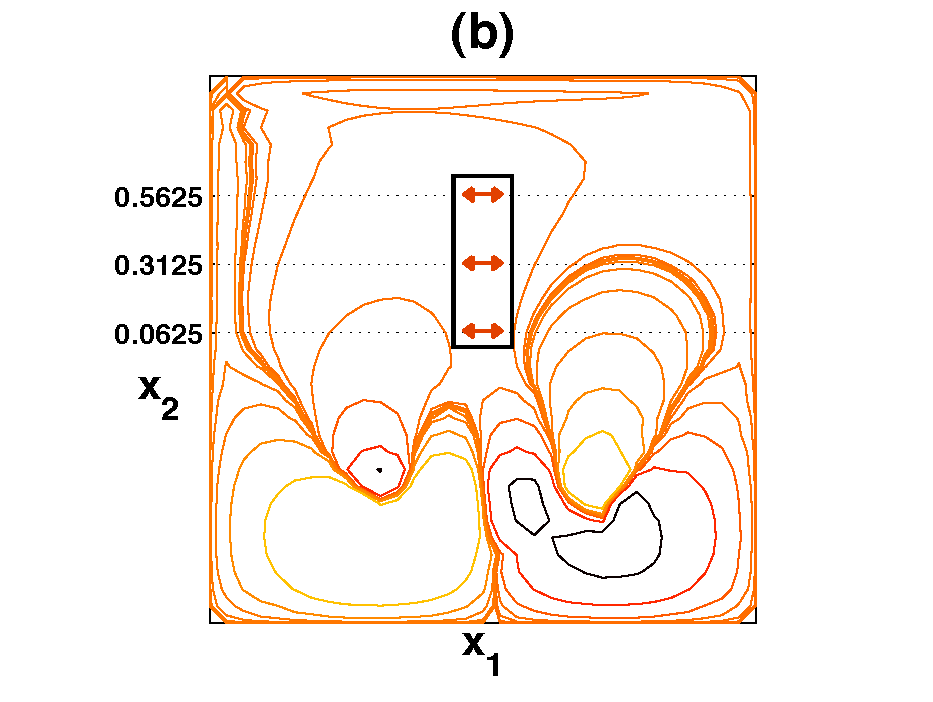
\includegraphics[width=6cm]{pics/fullOpti/new/stli_x2.pdf}
  \end{minipage}
   \caption{Velocity vector plot (a) and streamline plot (b) of the controlled Oseen driven cavity flow at time $t=0.1$, influenced by the input signal $u^{2*}$, optimized with respect to a uniform velocity distribution ($v_x = 0,~v_y=1$) within the time interval $[0,0.1]$ in the observation domain. The arrows in (a) indicate the positions of the extraction of the output signals belonging to $y^{2*}$, which are displayed in Figure \ref{x2res}.} 
\label{x2vest}
\end{figure}

\begin{figure}
\centering
 \begin{minipage}[b]{5cm}
    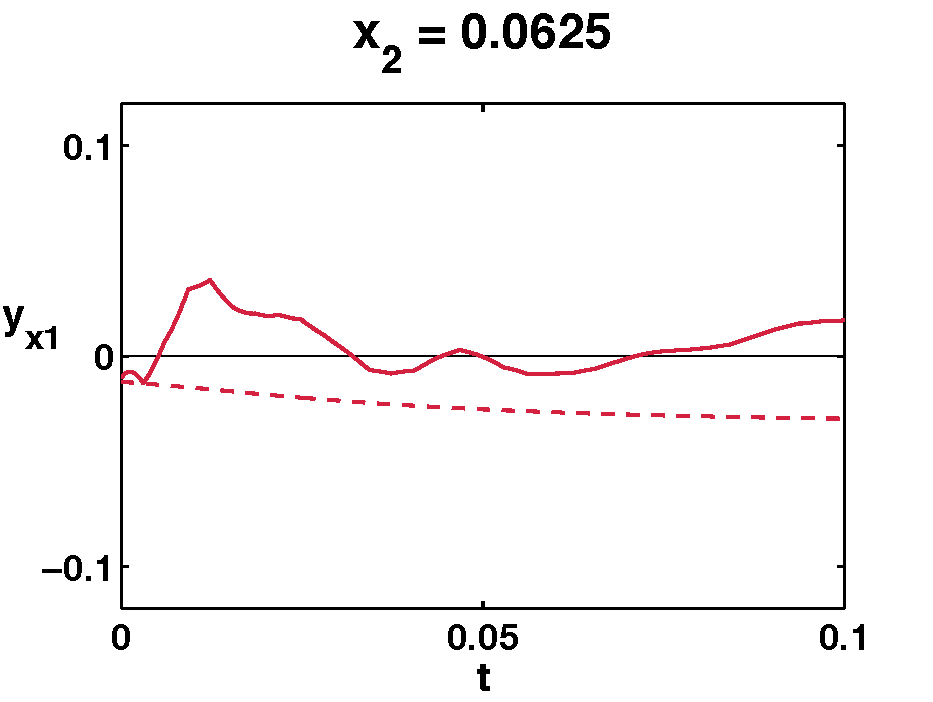
\includegraphics[width=5cm]{pics/fullOpti/new/x2_sigx2_1.pdf}  
  \end{minipage}
 \begin{minipage}[b]{5cm}
    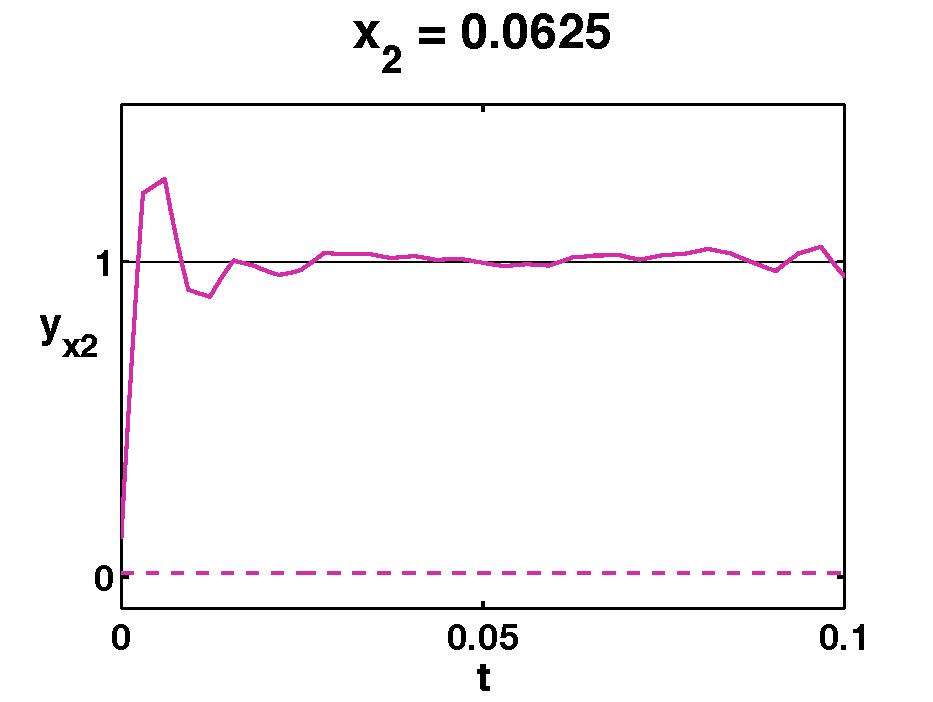
\includegraphics[width=5cm]{pics/fullOpti/new/x2_sigx22_1.pdf}  
  \end{minipage}
\vspace{0.3cm}
 \begin{minipage}[b]{5cm}
    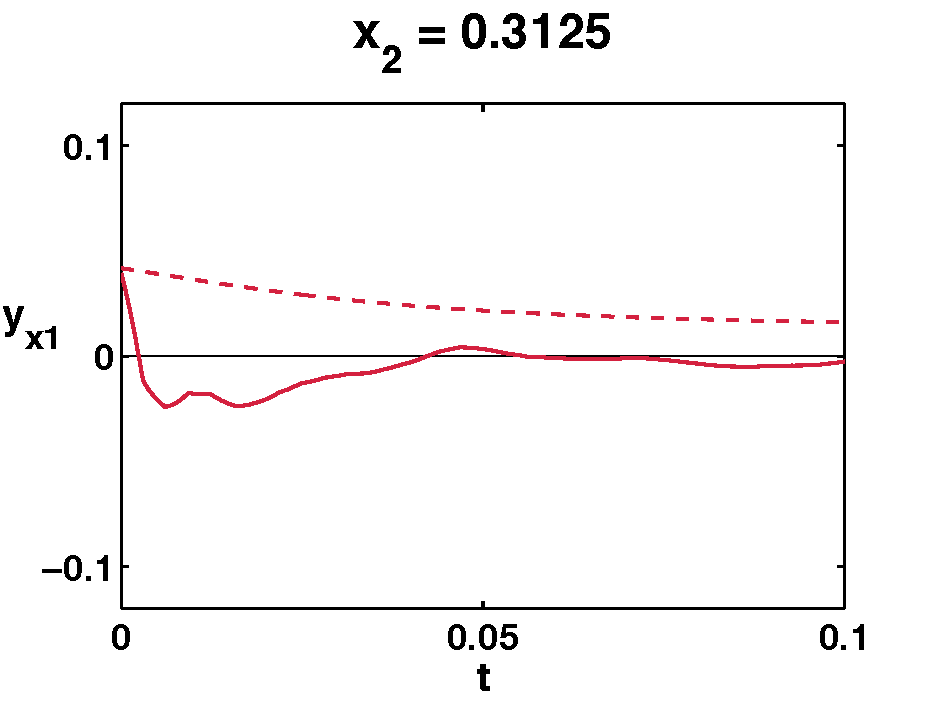
\includegraphics[width=5cm]{pics/fullOpti/new/x2_sigx2_2.pdf}  
  \end{minipage}
 \begin{minipage}[b]{5cm}
    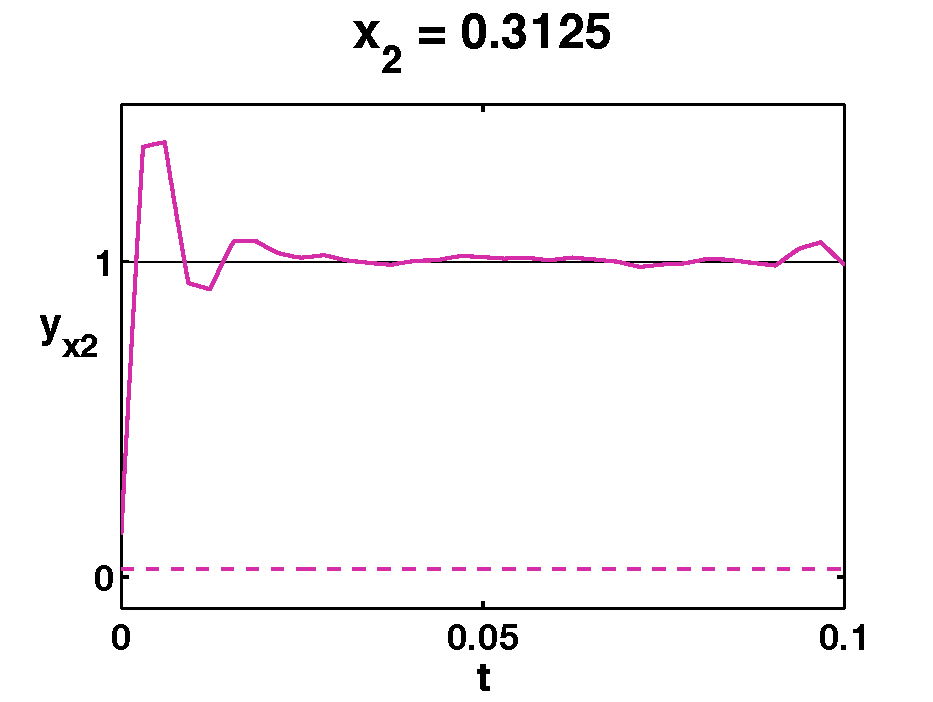
\includegraphics[width=5cm]{pics/fullOpti/new/x2_sigx22_2.pdf}  
  \end{minipage}
\vspace{0.3cm}
 \begin{minipage}[b]{5cm}
    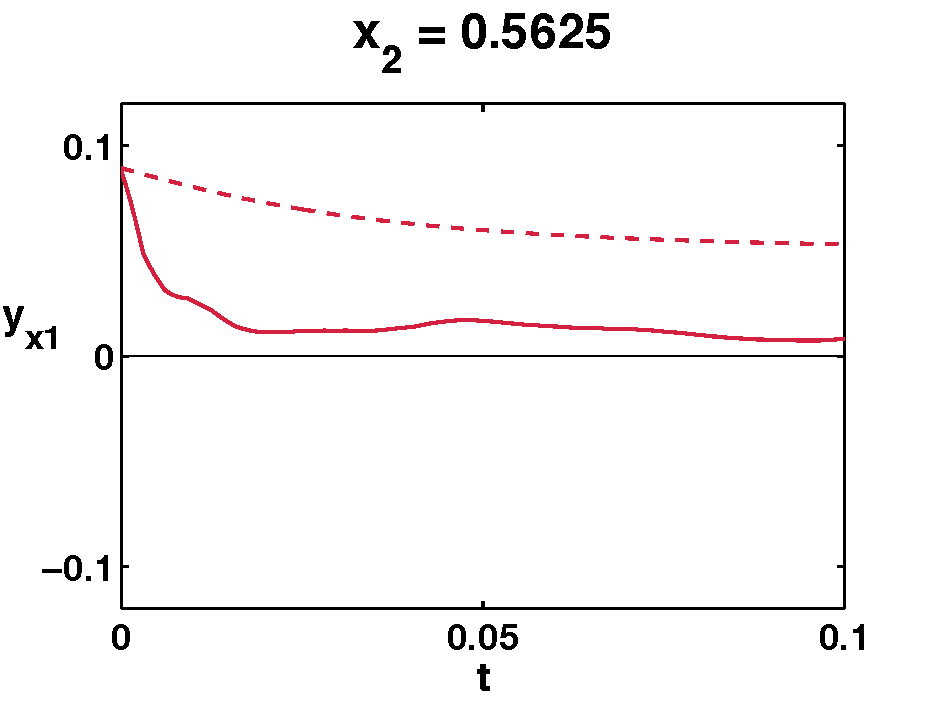
\includegraphics[width=5cm]{pics/fullOpti/new/x2_sigx2_3.pdf}  
  \end{minipage}
 \begin{minipage}[b]{5cm}
    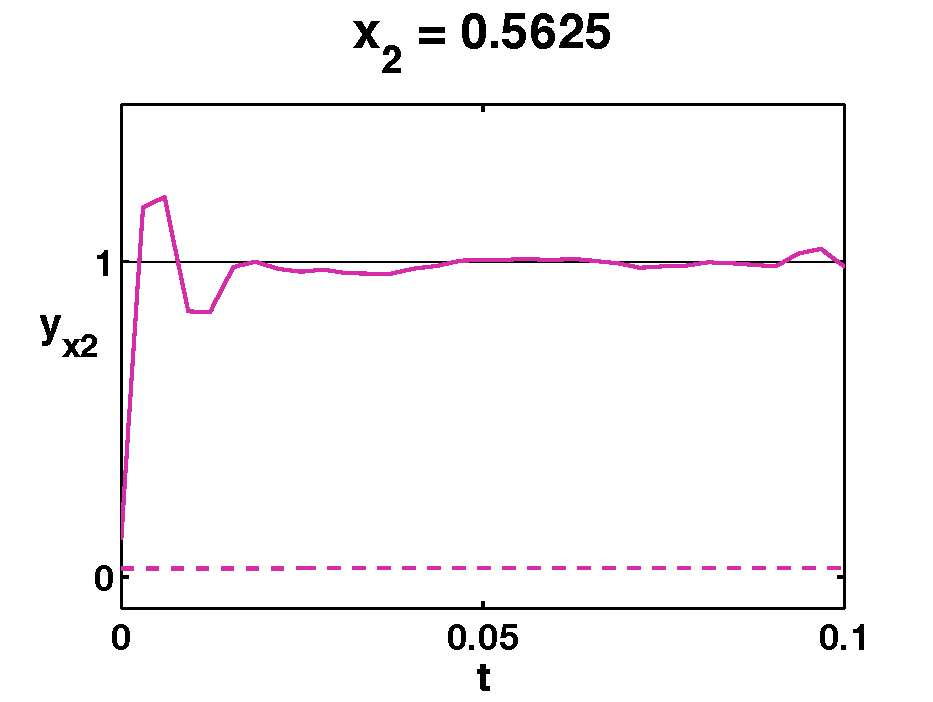
\includegraphics[width=5cm]{pics/fullOpti/new/x2_sigx22_3.pdf}  
  \end{minipage}
   \caption{6 components of the signal response $\mathbf y_h^{2*}$. The plots on the left-hand side show the $x_1$-component of the output at the sensor positions indicated in Figure \ref{x1vest} versus the time $t\in [0,0.1]$. The right-hand side displays the corresponding $x_2$-component. The dotted lines mark the corresponding ''uncontrolled`` outputs.} 
\label{x2res}
\end{figure}

Compared to the results for $\mathbf y_h^{1*}$ the plots in Figure \ref{x2res} show a smoother behaviour. This is possibly due to the fact, that in the second case the control acts more directly on the observation domain. 

Both optimization cases were set up without further considerations on the formulation of the optimization problem. Nevertheless the above results back the approach of using the Oseen equation in combination with discrete i/o mapping to solve optimal control problems in fluid mechanics. More significant results may be obtained by investigating the proper choice of the target funtional. For example, adding a penalizing term for the input, containing e.g. the norm $\norm {\mathbf u}$ of the input, possibly helps to damp the oscillations. Also the dependence of the optimization on the resolution of the input and output signals requires further investigation.


\chapter{Summary and Outlook}
The key results of this work are connected to the explicit solution \eqref{exsolos} formula for the spatially discretized Oseen equations. Treating the solution of the flow equations as a solution of a DAE establishes a direct relation between the input and the output for Oseen system with distributed control and observation. The closed form gives a base for error estimations directly considering the use of finite dimensional in- and outputs.

A second important implication of the formula concerns the necessary regularity of the right-hand side $\mathbf f_h$ and the control $\mathbf u_h$ appearing in the semidiscretized state equations. For a general discretization scheme with the corresponding matrix
\begin{equation*}
 E_{11} := [I-D^{-1}B^T[Q+BD^{-1}B^T]^{-1}B]D^{-1}M 
\end{equation*}
the formula requires for the velocity and the pressure solution $\mathbf f_h + \mathbf u_h$ in $\mathcal C[0,T]$ and in $\mathcal C^1[0,T]$, respectively. If only the velocity component is considered, the general case of $\ind E_{11}=2$ already admits the use of wavelets and lower order finite elements for the discretization of the input. However these regularity conditions are possibly too strong. Therefore a future task is to determine conditions for the spatial discretization schemes that ensure a $E_{11}$ of index $1$.

Another open task coming with the DAE theory is the proper treatment of the starting values. Actually the integration of the spatially discretized Oseen equations requires a consistent initial value. In the present case of linear equations with constant coefficients one can check the given initial value for consistency and if necessary do a correction as e.g. described in \cite[p. 309]{mehr}. This issue was excluded in the theoretical analysis and circumvented in the practical implementation by using a \textit{projection algorithm}. For a deeper understanding it may be worth investigating the choice of the corrected initial values influences the solution.

The use of the explicit solution formula to establish an i/o map for the distributed control of the Oseen system is straight forward. Also the numerical results backed the applicability of this approach. The optimal control of the spatially discretized Oseen system, however, has to be seen in the larger context of controlling the corresponding Navier-Stokes equations. As mentioned and illustrated in the introduction the optimal control of Oseen is a subcycle of a loop aiming at the optimal control of the NSEs.

\begin{figure}[htbp]
\begin{equation*}
\boxed{
 \xymatrix{
u_n  \ar[rr] & &*+=[F-,]\txt{~NSEs~ }\ar[dd] \ar[r] &C^Tv_n \stackrel{!}{=}y^* \ar[ddl]|-{\text{~~~~Linearization about $v_n$}}  \\  & & & \\
 & \bar u_n^k \ar[r] &*+=[F-,]\txt{~Oseen~ } \ar[r] &C^T\bar v_n^k \stackrel{!}{=}\bar y^* \ar[ld] \\
\bar u_{n}^* \ar[uuu]|- {~~n \leftarrow n+1} & &\framebox{Control} \ar [ll] \ar[lu]|- {k \leftarrow k+1 }  &
}
}
\end{equation*}
\caption{Scheme1: Optimal control of NSE by Oseen approximation with control unit in the inner loop}
\label{optscheme2}
\end{figure}

The mentioned above scheme with the control acting only in the inner iteration is shown in Figure \ref{optscheme2} and referred to in the following discussion as \textit{Scheme1}. A variant for further investigation  may be the coupling of the control directly to the NSEs and to use the Oseen equations to solve the nonlinear equations in the sense of a Newton-scheme. Note that this variation, illustrated in Figure \ref{optscheme3}, is not linear in the control.

\begin{figure}[htbp]
\begin{equation*}
\boxed{
 \xymatrix{
&  ~~~~~~~\framebox{$v_n^k \leftarrow v_n^{k+1}$}\ar@<2.5ex>[d]\\
u_n  \ar[r] &*+[F-,]\txt{ ~\\ ~NSEs $\rightarrow$ Oseen  \\ ~\scriptsize{(Newton iteration)}} \ar[r] \ar@<-6.5ex>[u] & C^Tv_n \stackrel{!}{=}y^* \ar[dl] \\  
u^*&  \framebox{Control} \ar [l] \ar[lu]|- {n \leftarrow n+1 } & \\
}
}
\end{equation*}
\caption{Optimal control of NSE by Oseen approximation with control unit in outer loop}
\label{optscheme3}
\end{figure}

Furthermore Scheme1 has to be checked for efficiency and robustness against other approaches, like the empirical \textit{black box} approaches. The term \textit{black box} means that the state equations are not analysed but considered as a deterministic system, delivering a certain output $y_k$ for a given input $u_k$. To find an optimum value $u^*$ the system response is computed for a finite set of inputs $u_i, ~i=1,\dotsc,N$. The resulting outputs $y_i$ are then analysed to identify a possibly improved $u_{N+1}$ e.g. by an extrapolation or a genetic algorithm. See Figure \ref{blackbox} for an illustration of the principle.

\begin{figure}[htbp]
\begin{equation*}
\boxed{
 \xymatrix{
\txt{$u_1$ \\ $\vdots $ \\ $u_N$} \Biggr \}  \ar@<-0.5ex>[r]\ar@<0.5ex>[r] &*+[F-,]\txt{ Solver} \ar@<-0.5ex>[r]\ar@<0.5ex>[r] & \Biggl \{ \txt{$y_1$ \\ $\vdots $ \\ $y_N$}  \ar@<-0.5ex>[ld]\ar@<0.5ex>[ld] \\  
u_{N+1} \ar[u]|- {~~~N \leftarrow N+1 } &  \framebox{Control} \ar [l] & \\
}
}
\end{equation*}
\caption{Black box approach for optimal control of a flow problem. Iteration directed by the control to find $u_{N+1}$ so that $v_{N+1}$ matches the target output $y^*$}
\label{blackbox}
\end{figure}


In applications to flow problems often the \textit{black box} is represented by a flow solver, solving the posed flow problem numerically. For large scale problems where a concise analysis is unaffordable this approach still delivers satisfying results, see e.g \cite{moi}.

 To motivate and to detect the potential of further developments of the here proposed methods, comparing studies with \textit{black box} approaches may be an interesting future task. It is likely that on linear problems the method of linear i/o mapping performs similarly to e.g. the \textit{black box} realizations provided by the \textsc{Matlab} control toolbox \cite{matconbo} or other linear models as e.g. presented in \cite{ljun}. 

A more significant comparison, in particular with state-of-the-art \textit{nonlinear model prediction control} (NMPC) as discussed e.g. in \cite{allgoewer2006,bock2006,bock2000a,hiku2}, has to include an estimation of the competitiveness of \textit{Scheme1} with respect to highly nonlinear flow systems.

\bibliography{dip_bib}

\end{document}
